\section{Anexo}

\subsection{Experimentos}
\label{sec:experimentos}
% All Libraries Memory Allocation
\DeclareRobustCommand{\AllLibrariesMemoryAllocationOnePlotLine}{
    %insertar imagen
    \begin{figure}[H]
        \centering
        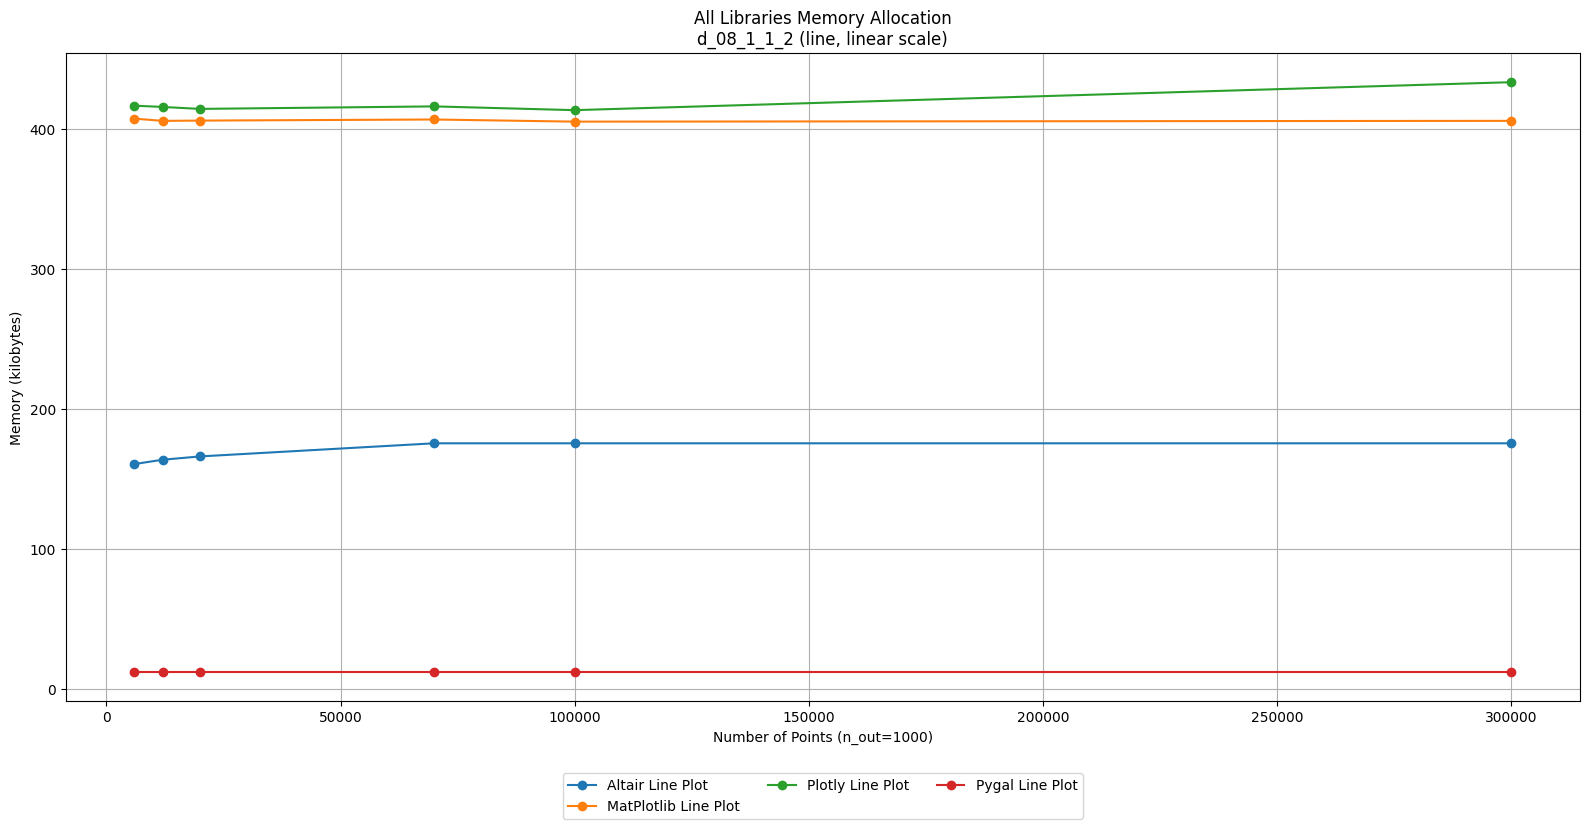
\includegraphics[width=1\textwidth]{anexo/exp/All Libraries Memory Allocation/plots/All Libraries Memory Allocation_d_08_1_1_2_linear_line.png}
        \caption[]{Gráfico de memoria asignada por las diferentes bibliotecas al crear un gráfico para el input \textbf{d\_08\_1\_1\_2}.}
        \label{fig:all_libraries_memory_allocation_plot_line_1}
    \end{figure}
}

\DeclareRobustCommand{\AllLibrariesMemoryAllocationOnePlotBar}{
    %insertar imagen
    \begin{figure}[H]
        \centering
        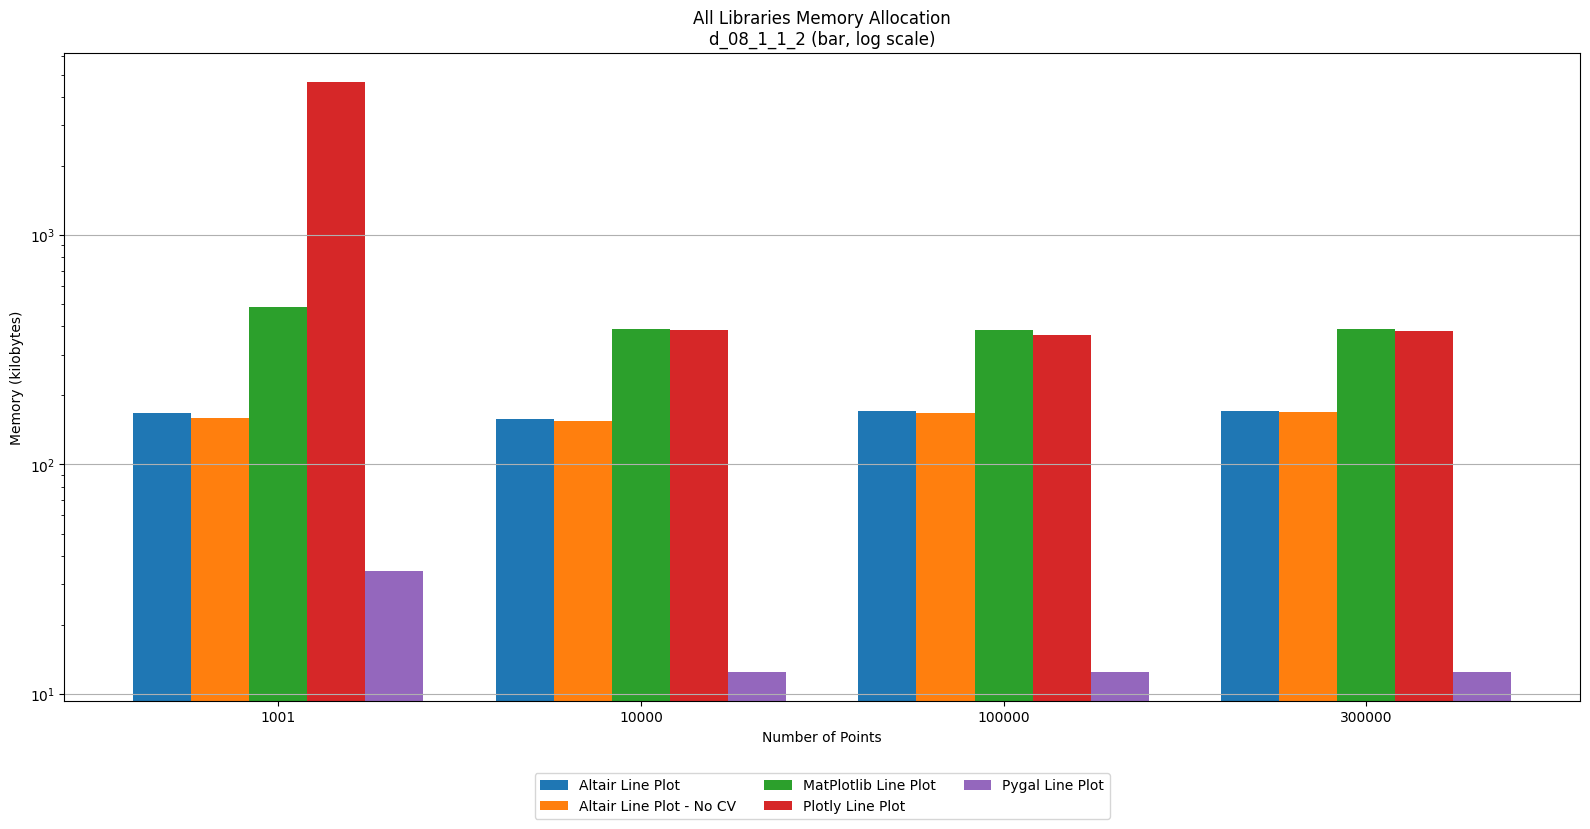
\includegraphics[width=1\textwidth]{anexo/exp/All Libraries Memory Allocation/bar_plots/All Libraries Memory Allocation_d_08_1_1_2_log_bar.png}
        \caption[]{Gráfico de memoria asignada por las diferentes bibliotecas al crear un gráfico para el input \textbf{d\_08\_1\_1\_2}.}
        \label{fig:all_libraries_memory_allocation_plot_bar_1}
    \end{figure}
}

\DeclareRobustCommand{\AllLibrariesMemoryAllocationTwoPlotLine}{
    %insertar imagen
    \begin{figure}[H]
        \centering
        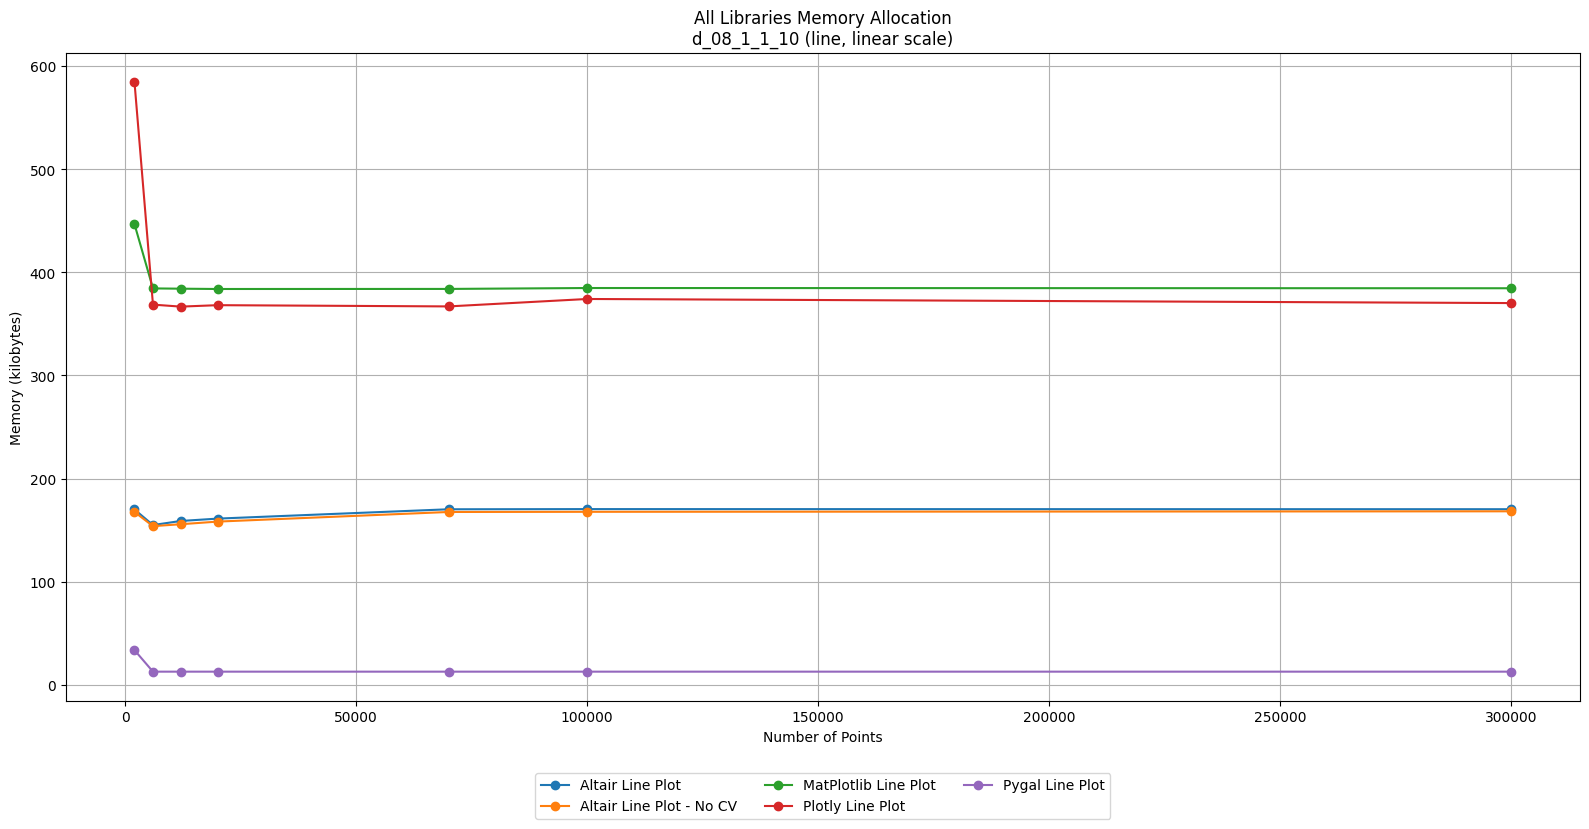
\includegraphics[width=1\textwidth]{anexo/exp/All Libraries Memory Allocation/plots/All Libraries Memory Allocation_d_08_1_1_10_linear_line.png}
        \caption[]{Gráfico de memoria asignada por las diferentes bibliotecas al crear un gráfico para el input \textbf{d\_08\_1\_1\_10}.}
        \label{fig:all_libraries_memory_allocation_plot_line_2}
    \end{figure}
}

\DeclareRobustCommand{\AllLibrariesMemoryAllocationTwoPlotBar}{
    %insertar imagen
    \begin{figure}[H]
        \centering
        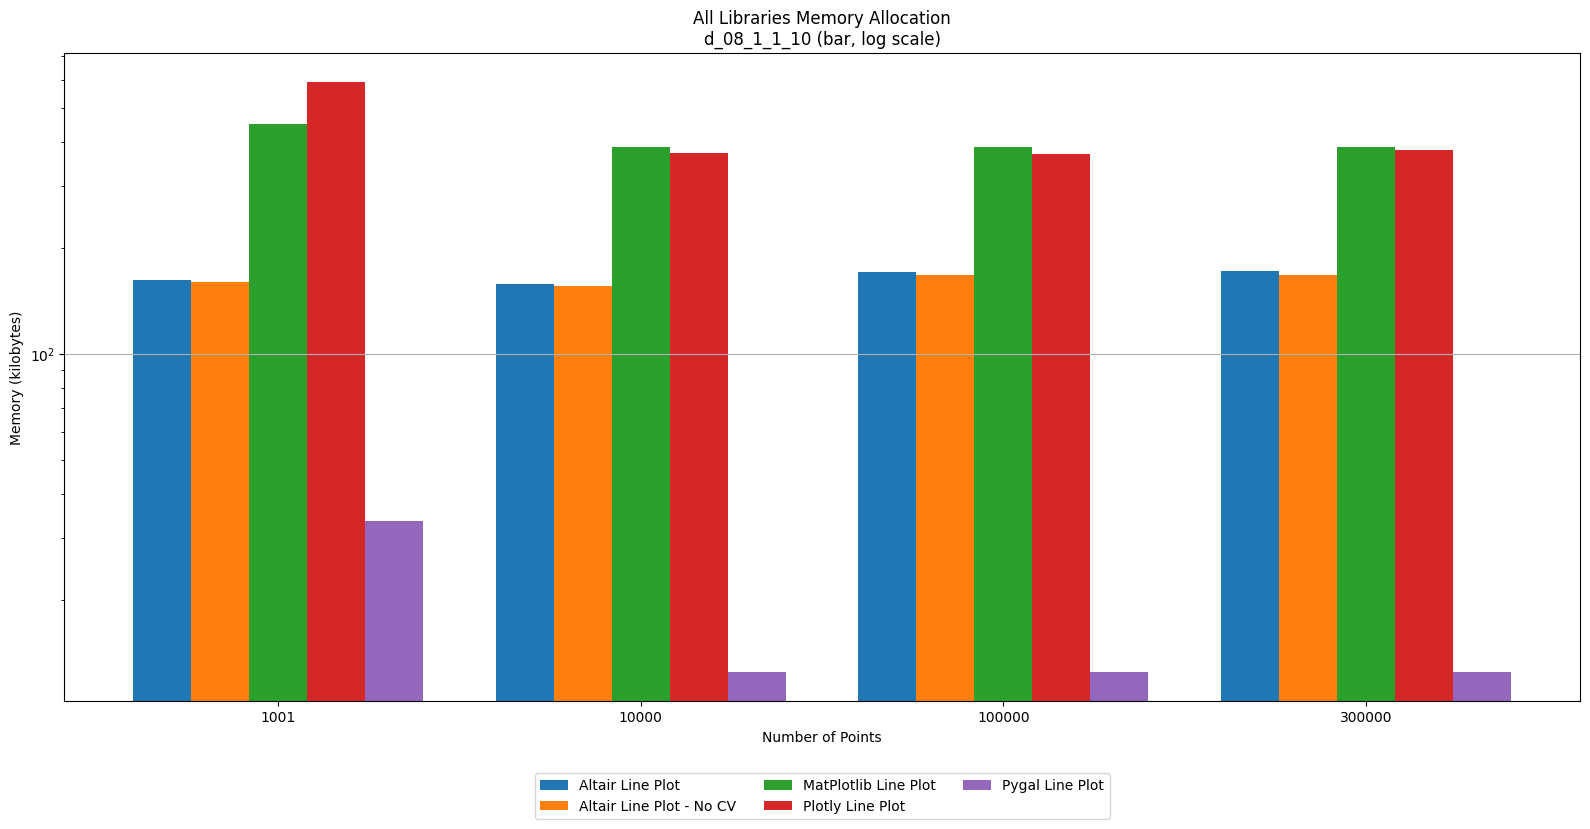
\includegraphics[width=1\textwidth]{anexo/exp/All Libraries Memory Allocation/bar_plots/All Libraries Memory Allocation_d_08_1_1_10_log_bar.png}
        \caption[]{Gráfico de memoria asignada por las diferentes bibliotecas al crear un gráfico para el input \textbf{d\_08\_1\_1\_10}.}
        \label{fig:all_libraries_memory_allocation_plot_bar_2}
    \end{figure}
}

\DeclareRobustCommand{\AllLibrariesMemoryAllocationThreePlotLine}{
    %insertar imagen
    \begin{figure}[H]
        \centering
        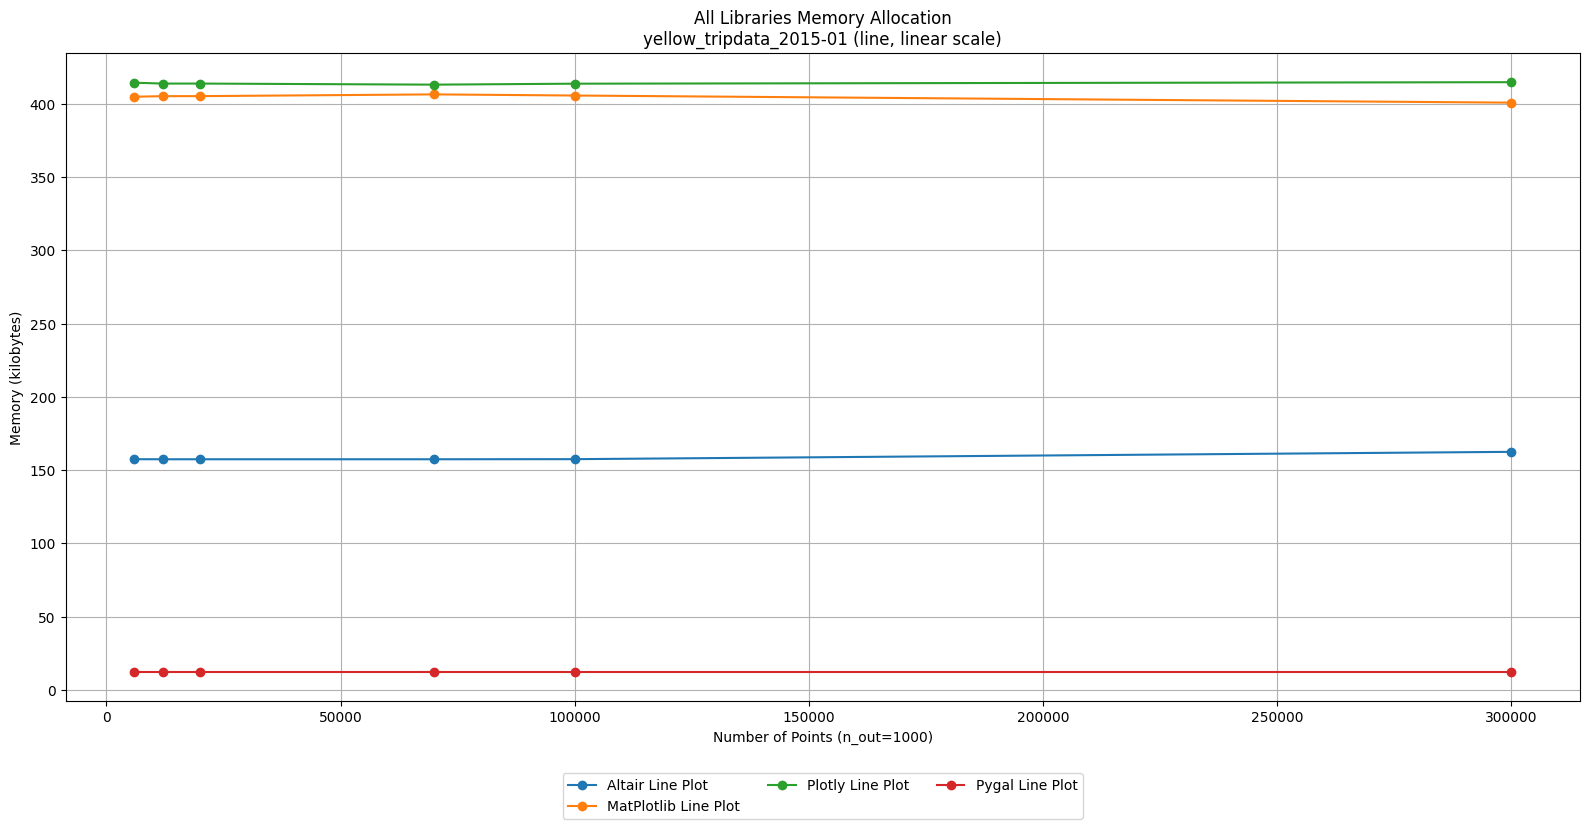
\includegraphics[width=1\textwidth]{anexo/exp/All Libraries Memory Allocation/plots/All Libraries Memory Allocation_yellow_tripdata_2015-01_linear_line.png}
        \caption[]{Gráfico de memoria asignada por las diferentes bibliotecas al crear un gráfico para el input \textbf{yellow\_tripdata\_2015\_01}.}
        \label{fig:all_libraries_memory_allocation_plot_line_3}
    \end{figure}
}

\DeclareRobustCommand{\AllLibrariesMemoryAllocationThreePlotBar}{
    %insertar imagen
    \begin{figure}[H]
        \centering
        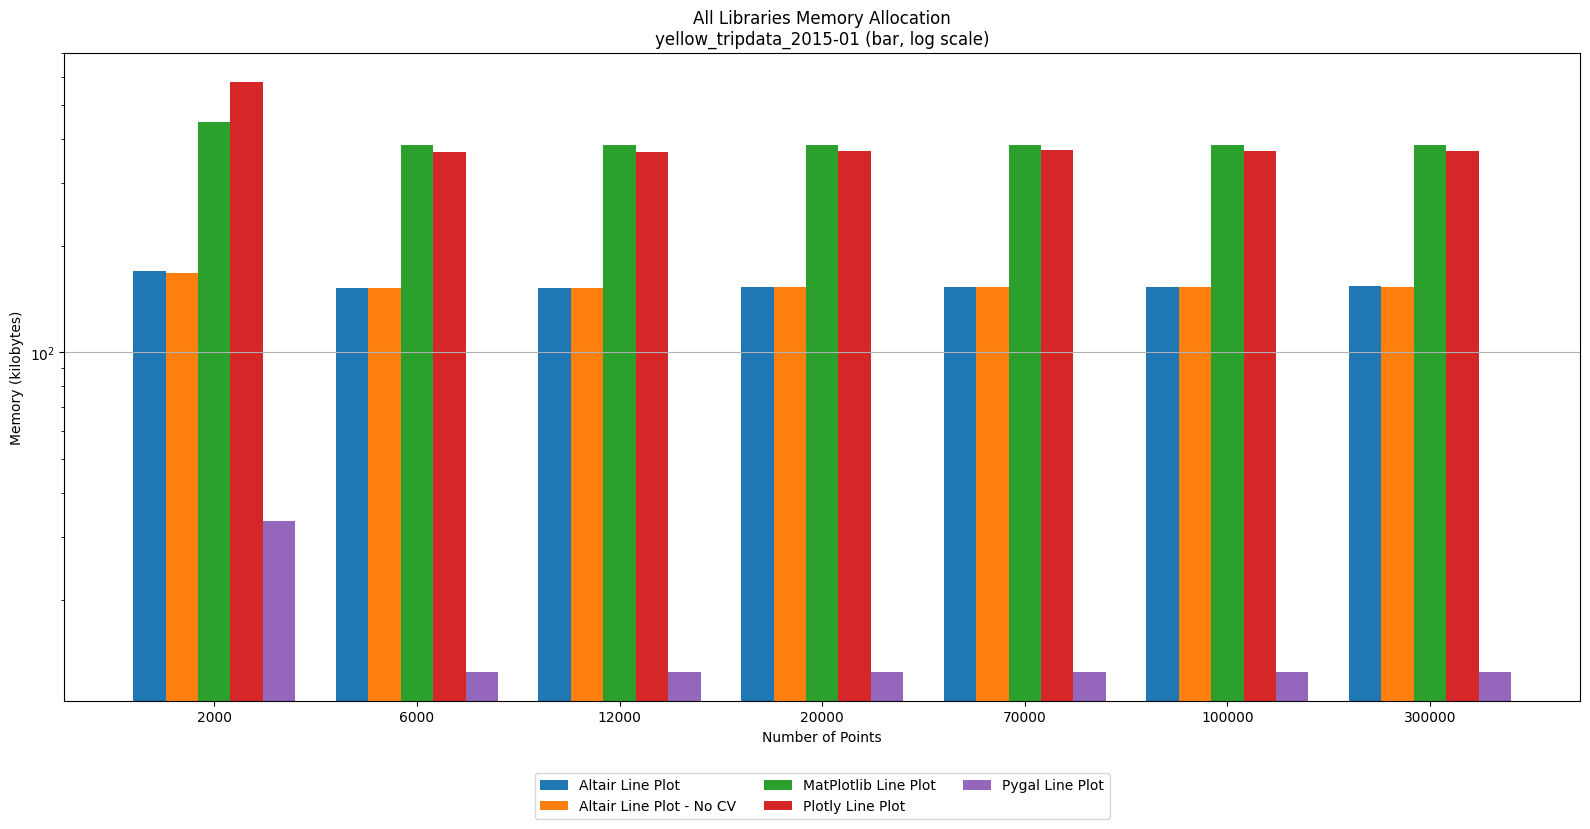
\includegraphics[width=1\textwidth]{anexo/exp/All Libraries Memory Allocation/bar_plots/All Libraries Memory Allocation_yellow_tripdata_2015-01_log_bar.png}
        \caption[]{Gráfico de memoria asignada por las diferentes bibliotecas al crear un gráfico para el input \textbf{yellow\_tripdata\_2015\_01}.}
        \label{fig:all_libraries_memory_allocation_plot_bar_3}
    \end{figure}
}




% All Libraries Time Comparison
\DeclareRobustCommand{\AllLibrariesTimeComparisonOnePlotLine}{
    %insertar imagen
    \begin{figure}[H]
        \centering
        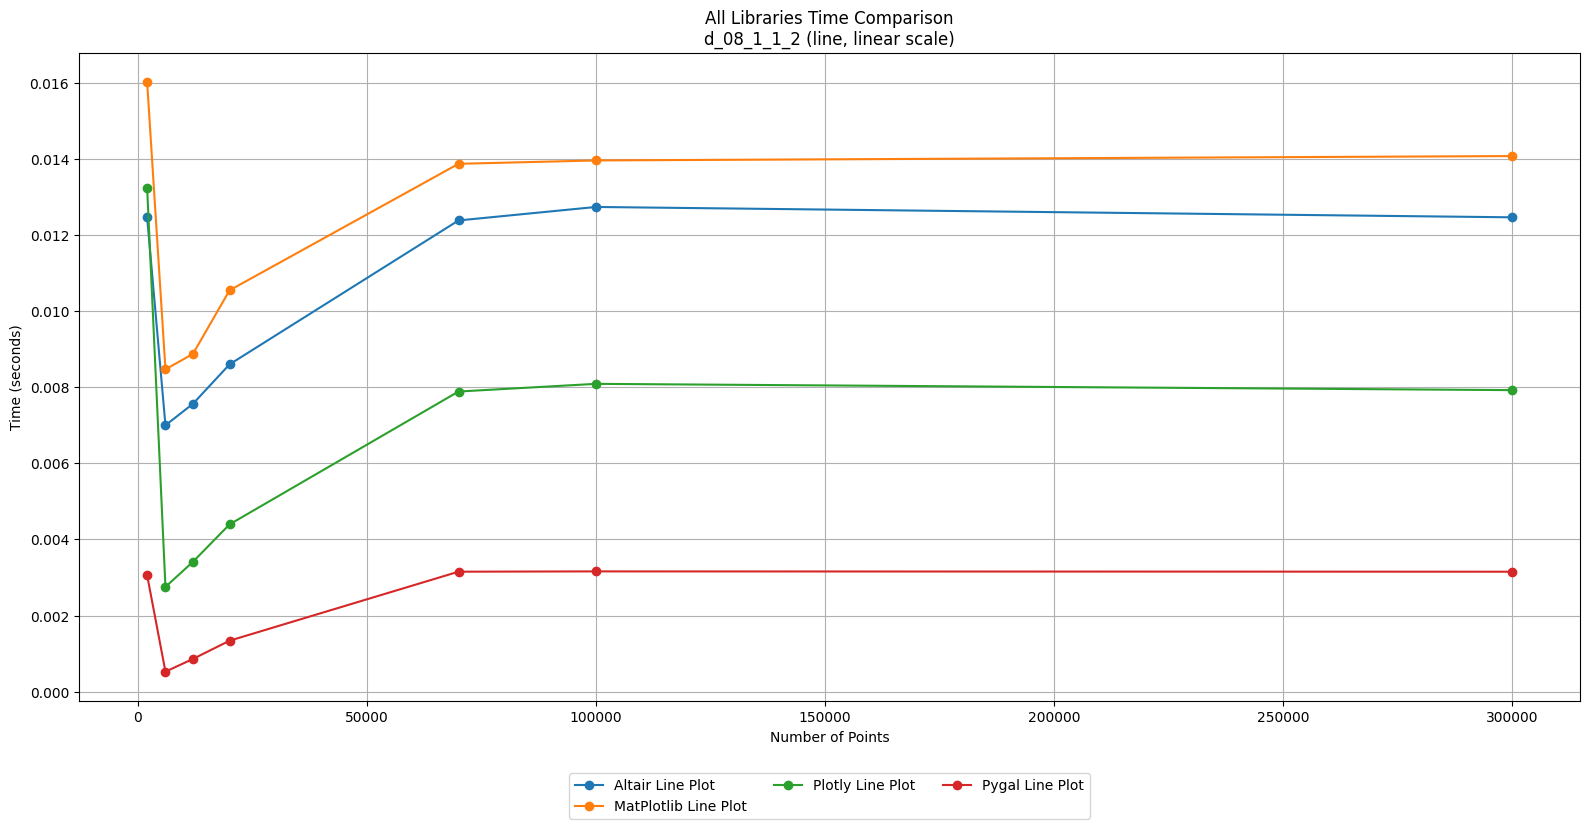
\includegraphics[width=1\textwidth]{anexo/exp/All Libraries Time Comparison/plots/All Libraries Time Comparison_d_08_1_1_2_linear_line.png}
        \caption[]{Gráfico de tiempo de ejecución de las diferentes bibliotecas al crear un gráfico para el input \textbf{d\_08\_1\_1\_2}.}
        \label{fig:all_libraries_time_comparison_plot_line_1}
    \end{figure}
}

\DeclareRobustCommand{\AllLibrariesTimeComparisonOnePlotBar}{
    %insertar imagen
    \begin{figure}[H]
        \centering
        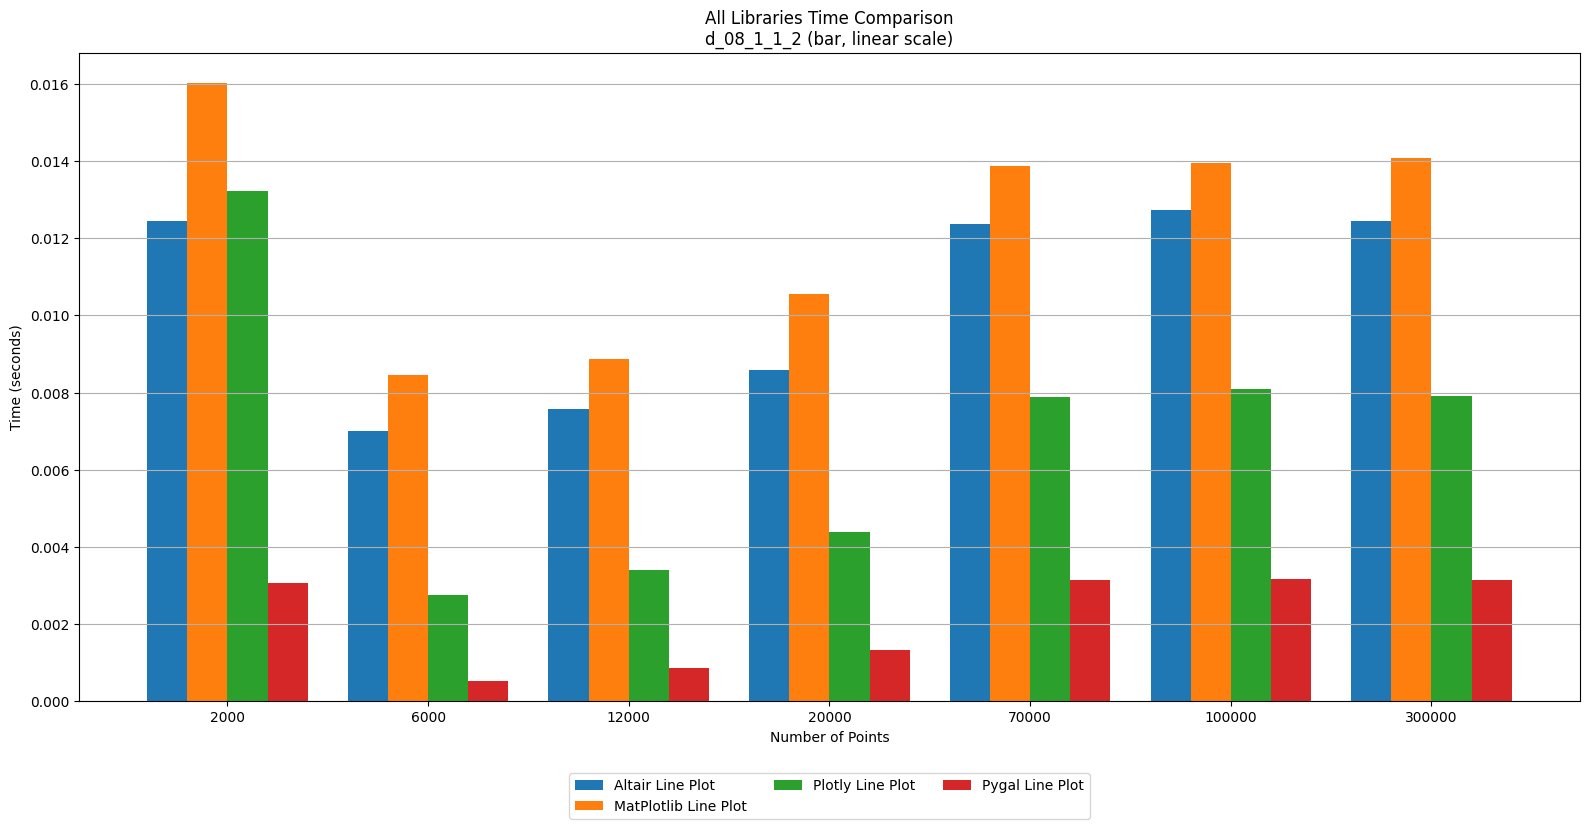
\includegraphics[width=1\textwidth]{anexo/exp/All Libraries Time Comparison/bar_plots/All Libraries Time Comparison_d_08_1_1_2_linear_bar.png}
        \caption[]{Gráfico de tiempo de ejecución de las diferentes bibliotecas al crear un gráfico para el input \textbf{d\_08\_1\_1\_2}.}
        \label{fig:all_libraries_time_comparison_plot_bar_1}
    \end{figure}
}

\DeclareRobustCommand{\AllLibrariesTimeComparisonTwoPlotLine}{
    %insertar imagen
    \begin{figure}[H]
        \centering
        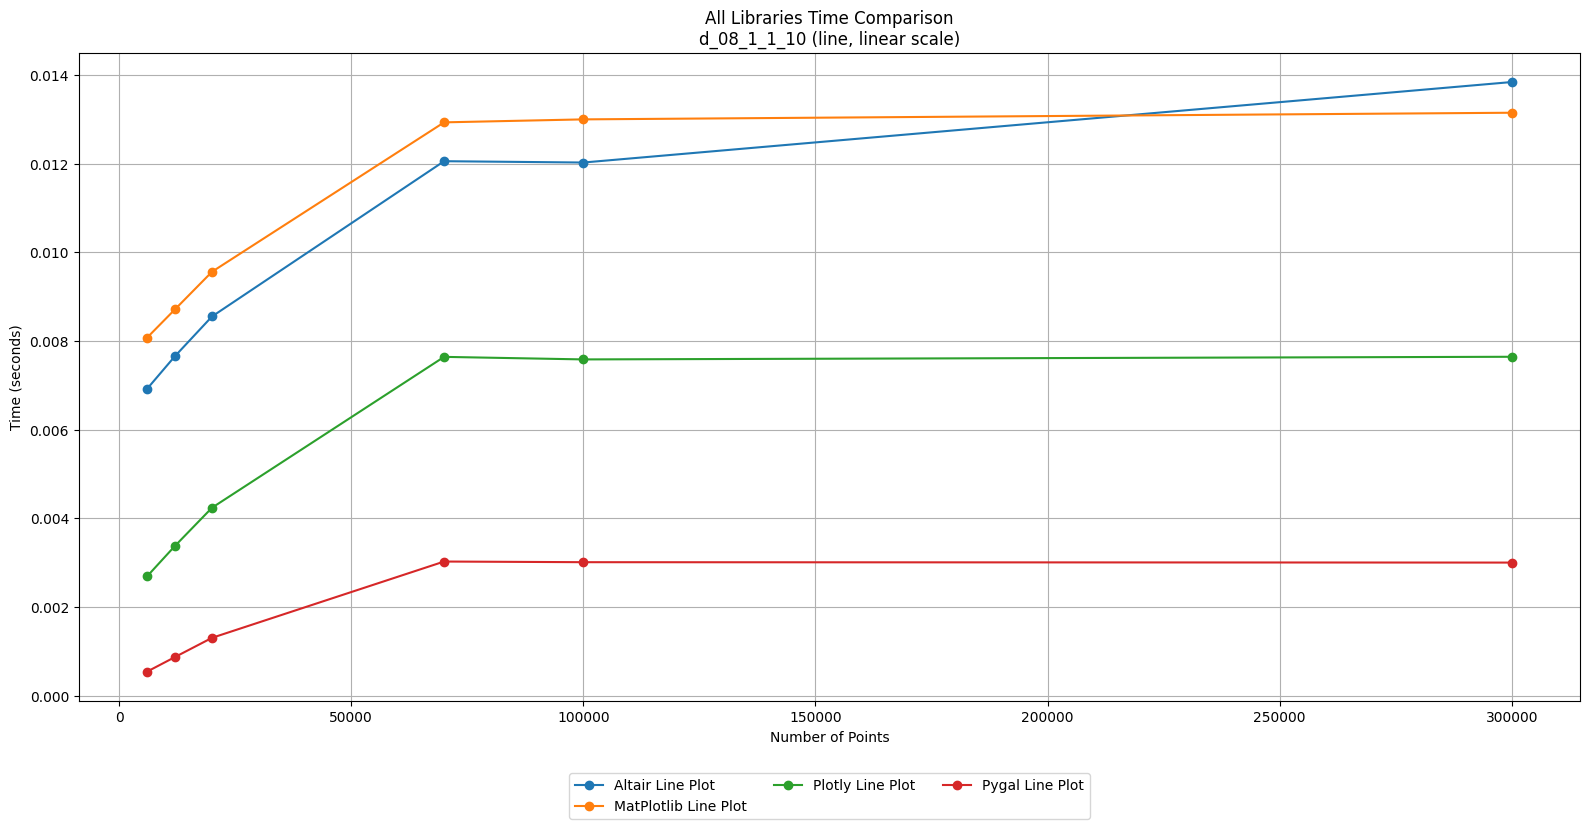
\includegraphics[width=1\textwidth]{anexo/exp/All Libraries Time Comparison/plots/All Libraries Time Comparison_d_08_1_1_10_linear_line.png}
        \caption[]{Gráfico de tiempo de ejecución de las diferentes bibliotecas al crear un gráfico para el input \textbf{d\_08\_1\_1\_10}.}
        \label{fig:all_libraries_time_comparison_plot_line_2}
    \end{figure}
}

\DeclareRobustCommand{\AllLibrariesTimeComparisonTwoPlotBar}{
    %insertar imagen
    \begin{figure}[H]
        \centering
        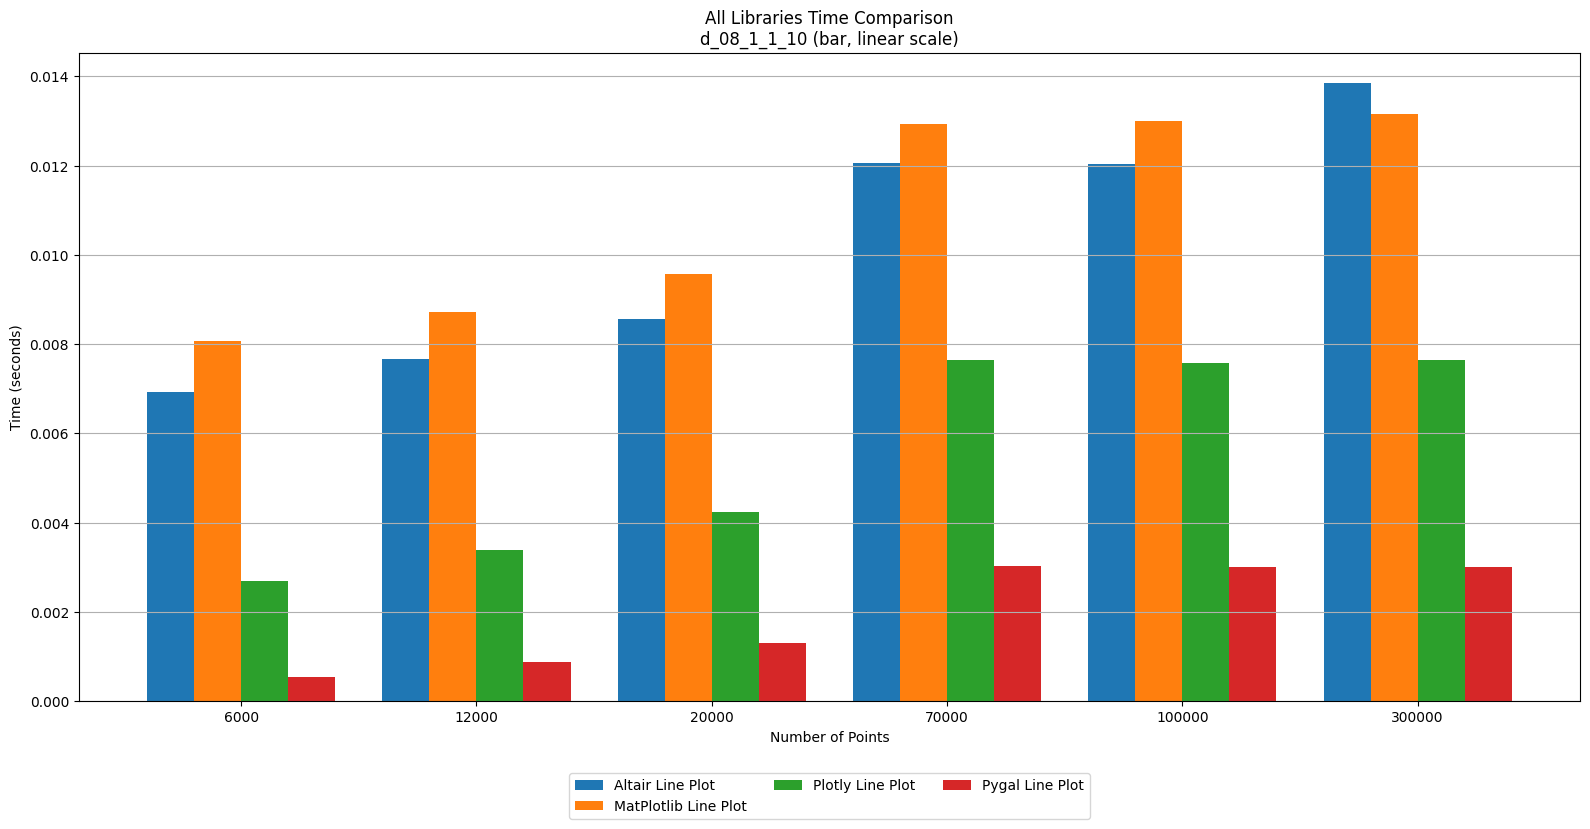
\includegraphics[width=1\textwidth]{anexo/exp/All Libraries Time Comparison/bar_plots/All Libraries Time Comparison_d_08_1_1_10_linear_bar.png}
        \caption[]{Gráfico de tiempo de ejecución de las diferentes bibliotecas al crear un gráfico para el input \textbf{d\_08\_1\_1\_10}.}
        \label{fig:all_libraries_time_comparison_plot_bar_2}
    \end{figure}
}

\DeclareRobustCommand{\AllLibrariesTimeComparisonThreePlotLine}{
    %insertar imagen
    \begin{figure}[H]
        \centering
        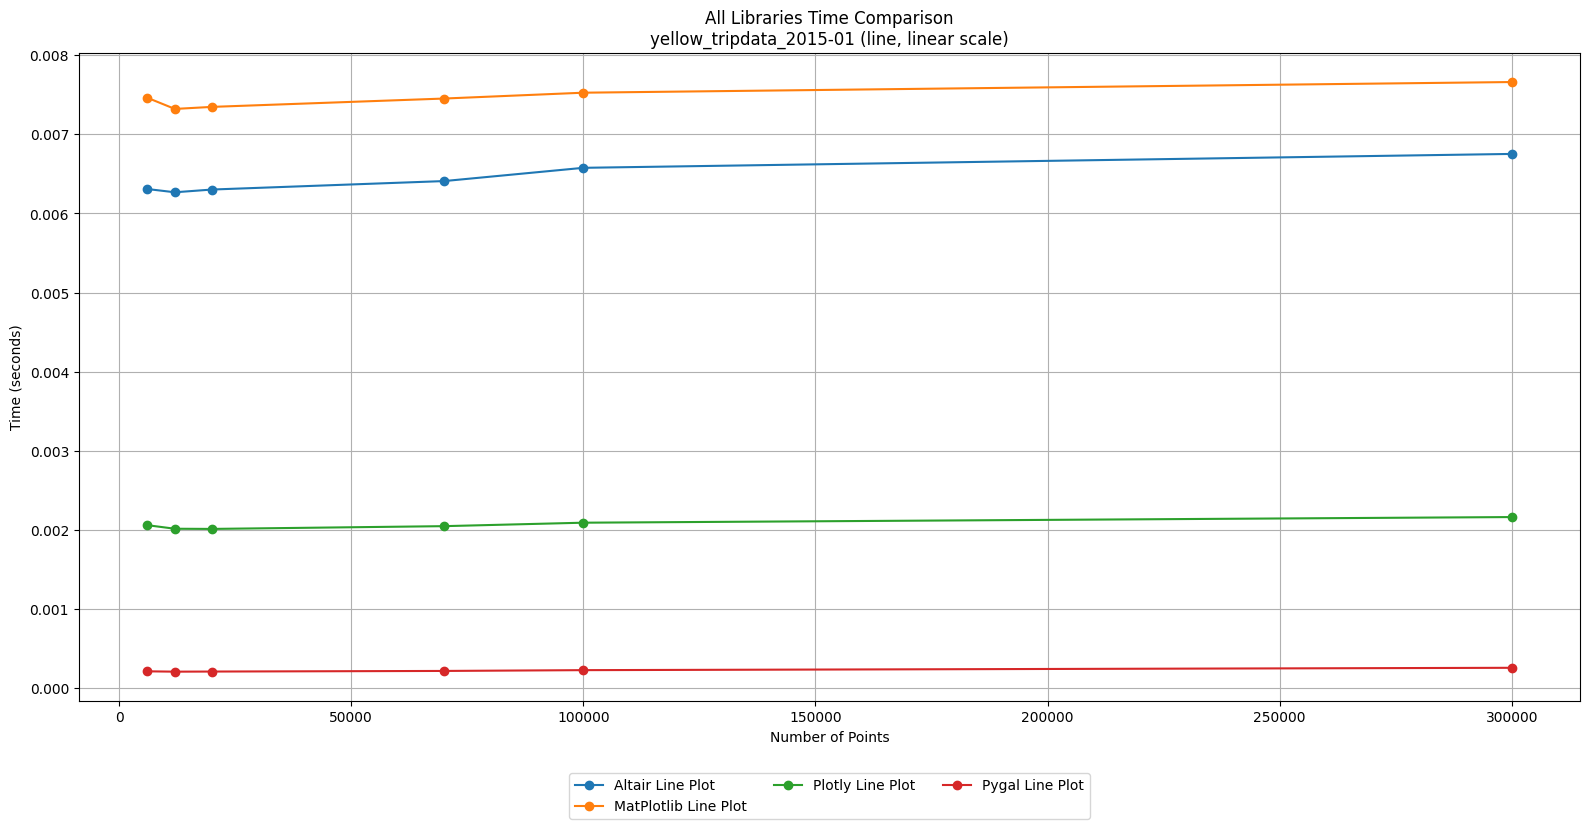
\includegraphics[width=1\textwidth]{anexo/exp/All Libraries Time Comparison/plots/All Libraries Time Comparison_yellow_tripdata_2015-01_linear_line.png}
        \caption[]{Gráfico de tiempo de ejecución de las diferentes bibliotecas al crear un gráfico para el input \textbf{yellow\_tripdata\_2015\_01}.}
        \label{fig:all_libraries_time_comparison_plot_line_3}
    \end{figure}
}

\DeclareRobustCommand{\AllLibrariesTimeComparisonThreePlotBar}{
    %insertar imagen
    \begin{figure}[H]
        \centering
        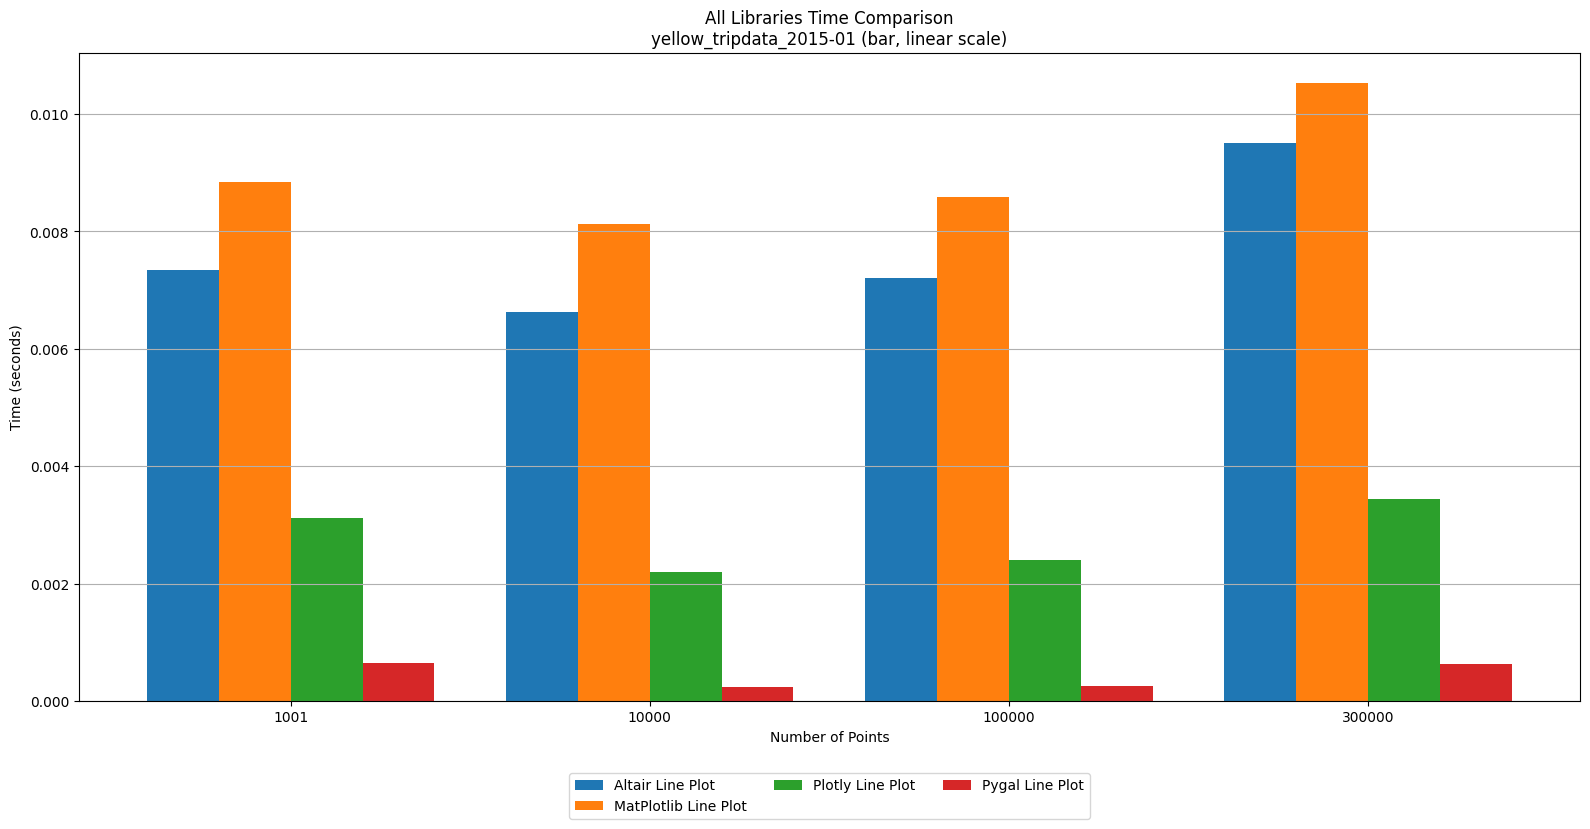
\includegraphics[width=1\textwidth]{anexo/exp/All Libraries Time Comparison/bar_plots/All Libraries Time Comparison_yellow_tripdata_2015-01_linear_bar.png}
        \caption[]{Gráfico de tiempo de ejecución de las diferentes bibliotecas al crear un gráfico para el input \textbf{yellow\_tripdata\_2015\_01}.}
        \label{fig:all_libraries_time_comparison_plot_bar_3}
    \end{figure}
}

Building Time Comparison
\DeclareRobustCommand{\BuildingTimeComparisonOnePlotLine}{
    %insertar imagen
    \begin{figure}[H]
        \centering
        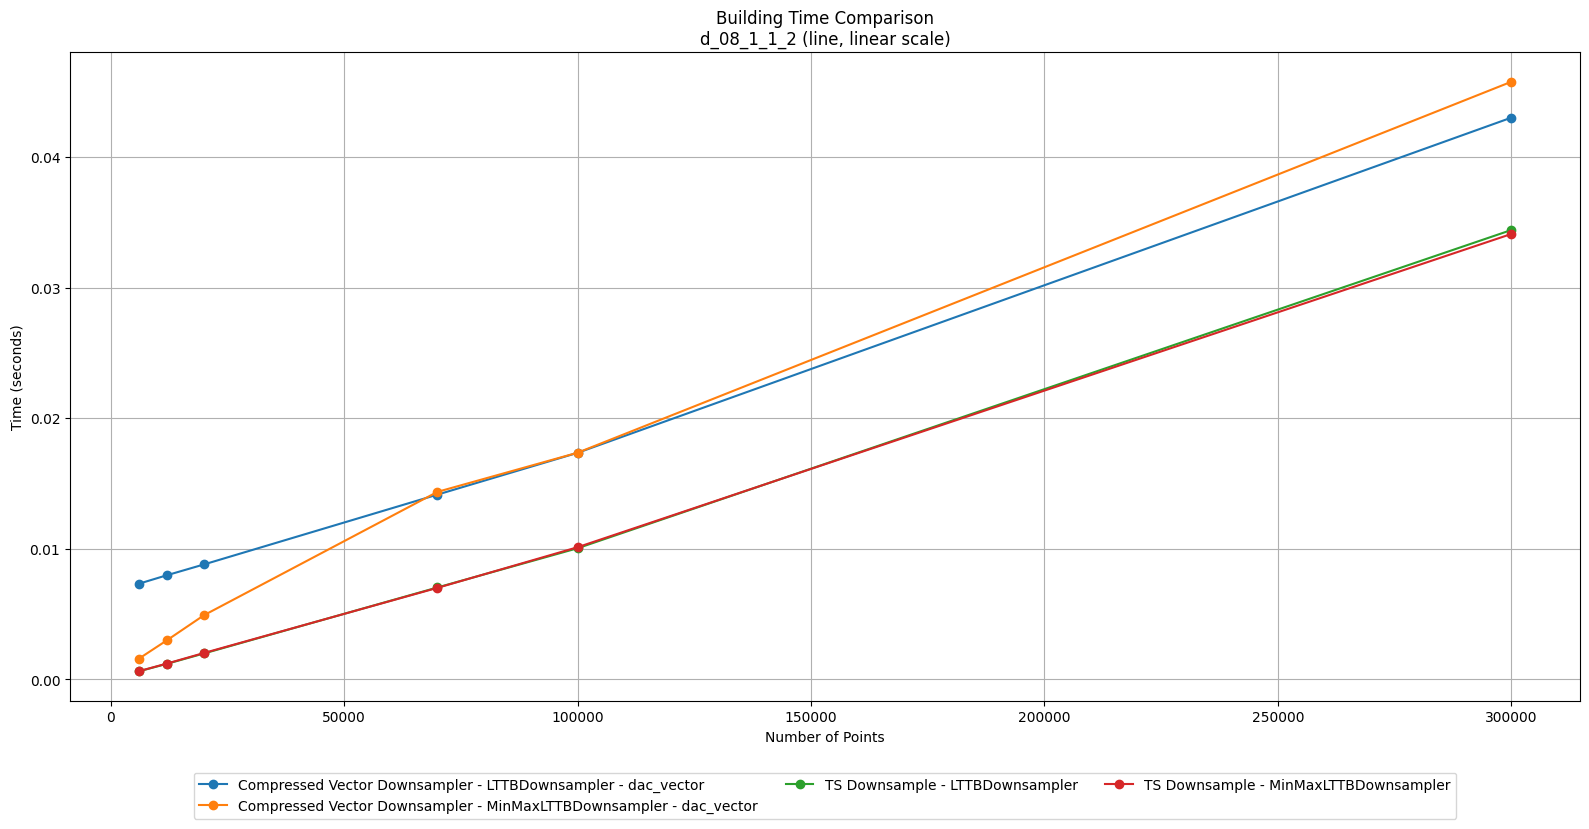
\includegraphics[width=1\textwidth]{anexo/exp/Building Time Comparison/plots/Building Time Comparison_d_08_1_1_2_linear_line.png}
        \caption[]{Gráfico de tiempo de construcción de las diferentes bibliotecas para el input \textbf{d\_08\_1\_1\_2}.}
        \label{fig:building_time_comparison_plot_line_1}
    \end{figure}
}

\DeclareRobustCommand{\BuildingTimeComparisonOnePlotBar}{
    %insertar imagen
    \begin{figure}[H]
        \centering
        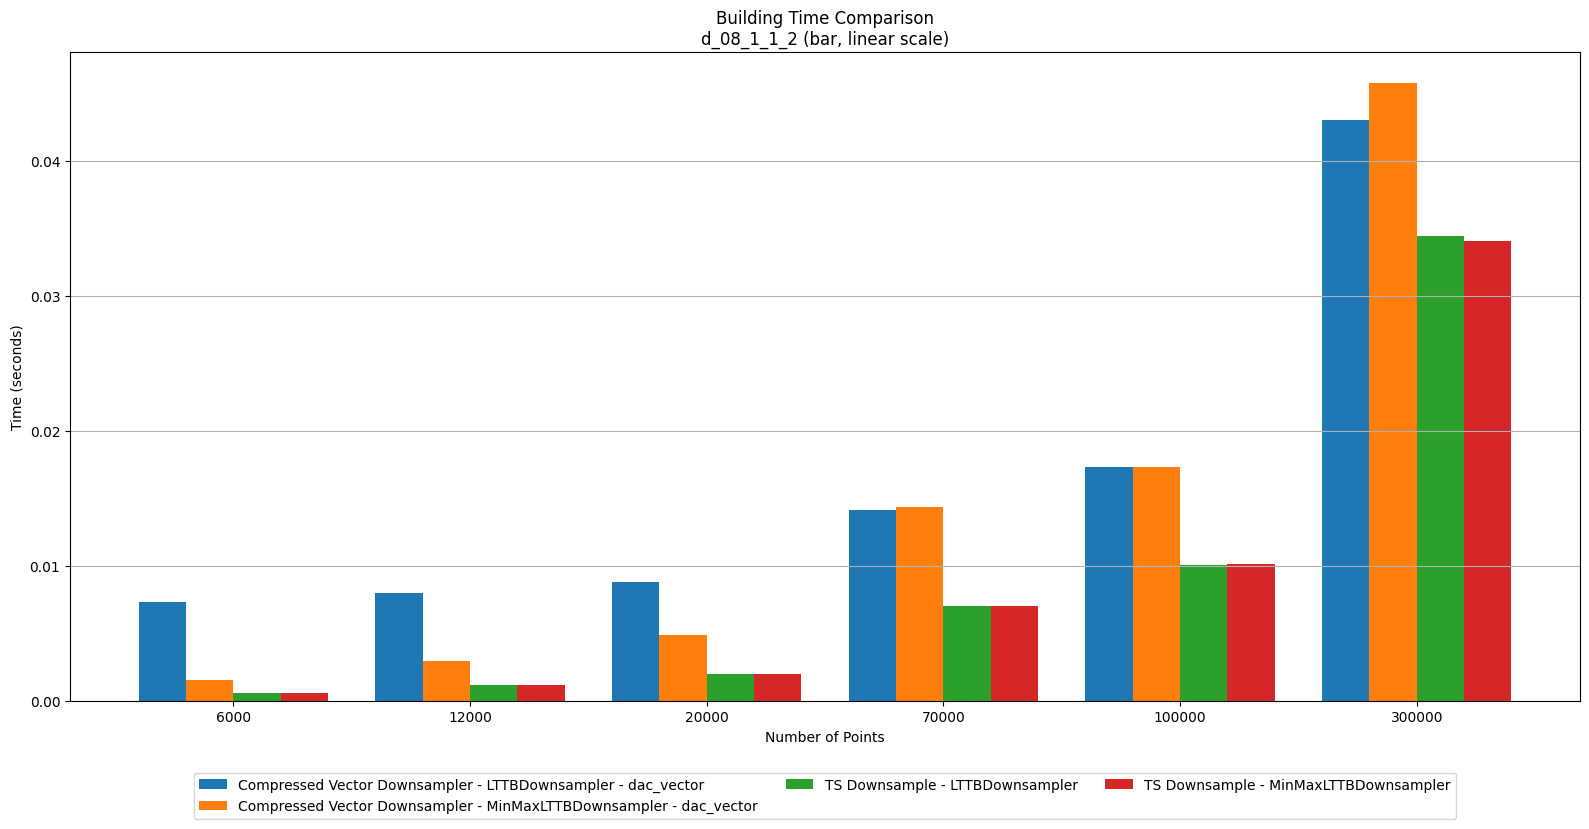
\includegraphics[width=1\textwidth]{anexo/exp/Building Time Comparison/bar_plots/Building Time Comparison_d_08_1_1_2_linear_bar.png}
        \caption[]{Gráfico de tiempo de construcción de las diferentes bibliotecas para el input \textbf{d\_08\_1\_1\_2}.}
        \label{fig:building_time_comparison_plot_bar_1}
    \end{figure}
}

\DeclareRobustCommand{\BuildingTimeComparisonTwoPlotLine}{
    %insertar imagen
    \begin{figure}[H]
        \centering
        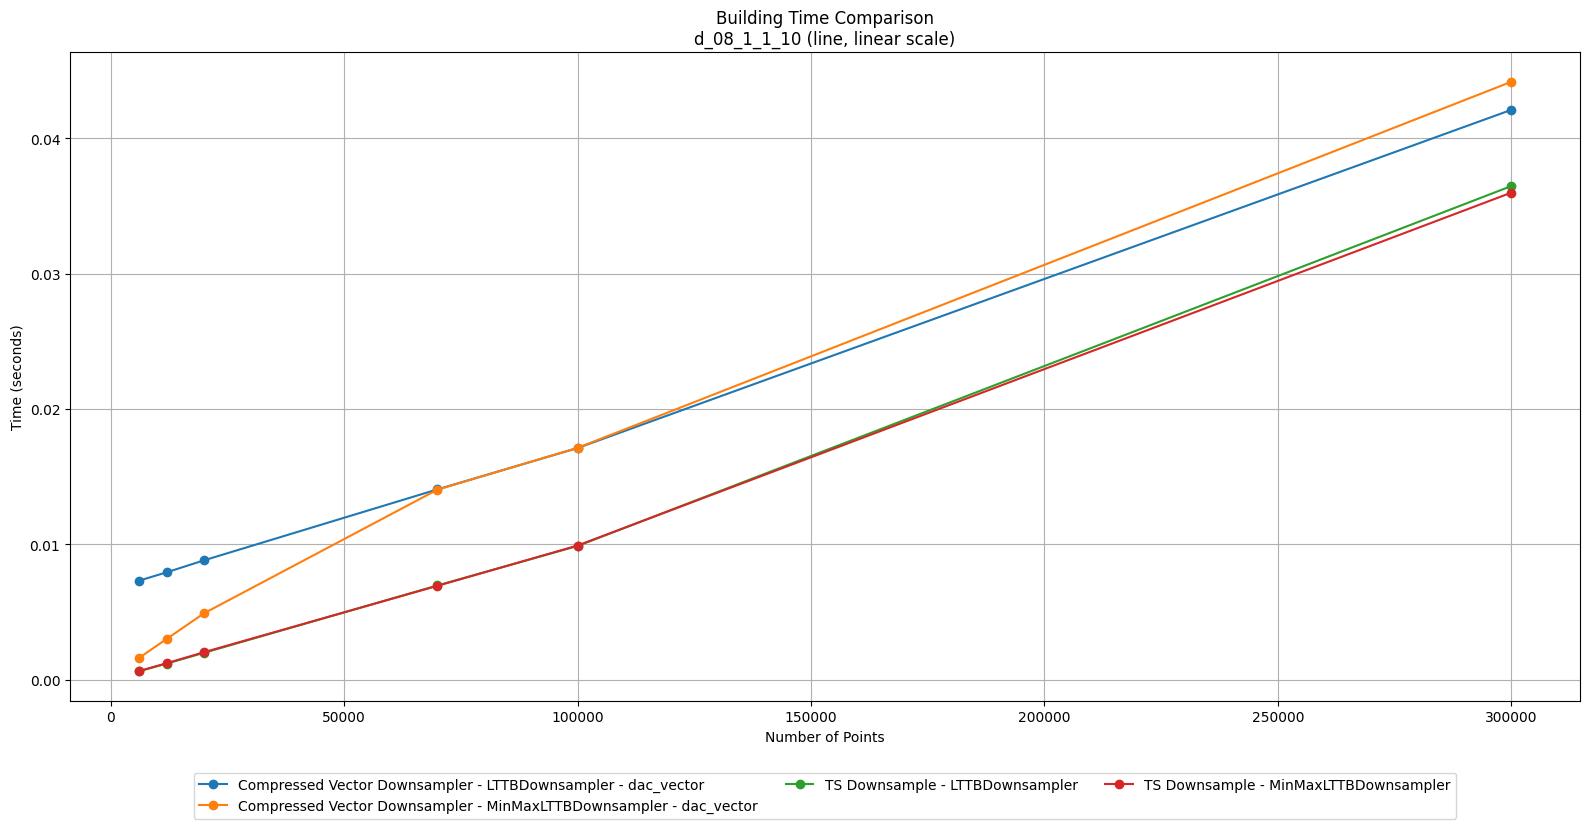
\includegraphics[width=1\textwidth]{anexo/exp/Building Time Comparison/plots/Building Time Comparison_d_08_1_1_10_linear_line.png}
        \caption[]{Gráfico de tiempo de construcción de las diferentes bibliotecas para el input \textbf{d\_08\_1\_1\_10}.}
        \label{fig:building_time_comparison_plot_line_2}
    \end{figure}
}

\DeclareRobustCommand{\BuildingTimeComparisonTwoPlotBar}{
    %insertar imagen
    \begin{figure}[H]
        \centering
        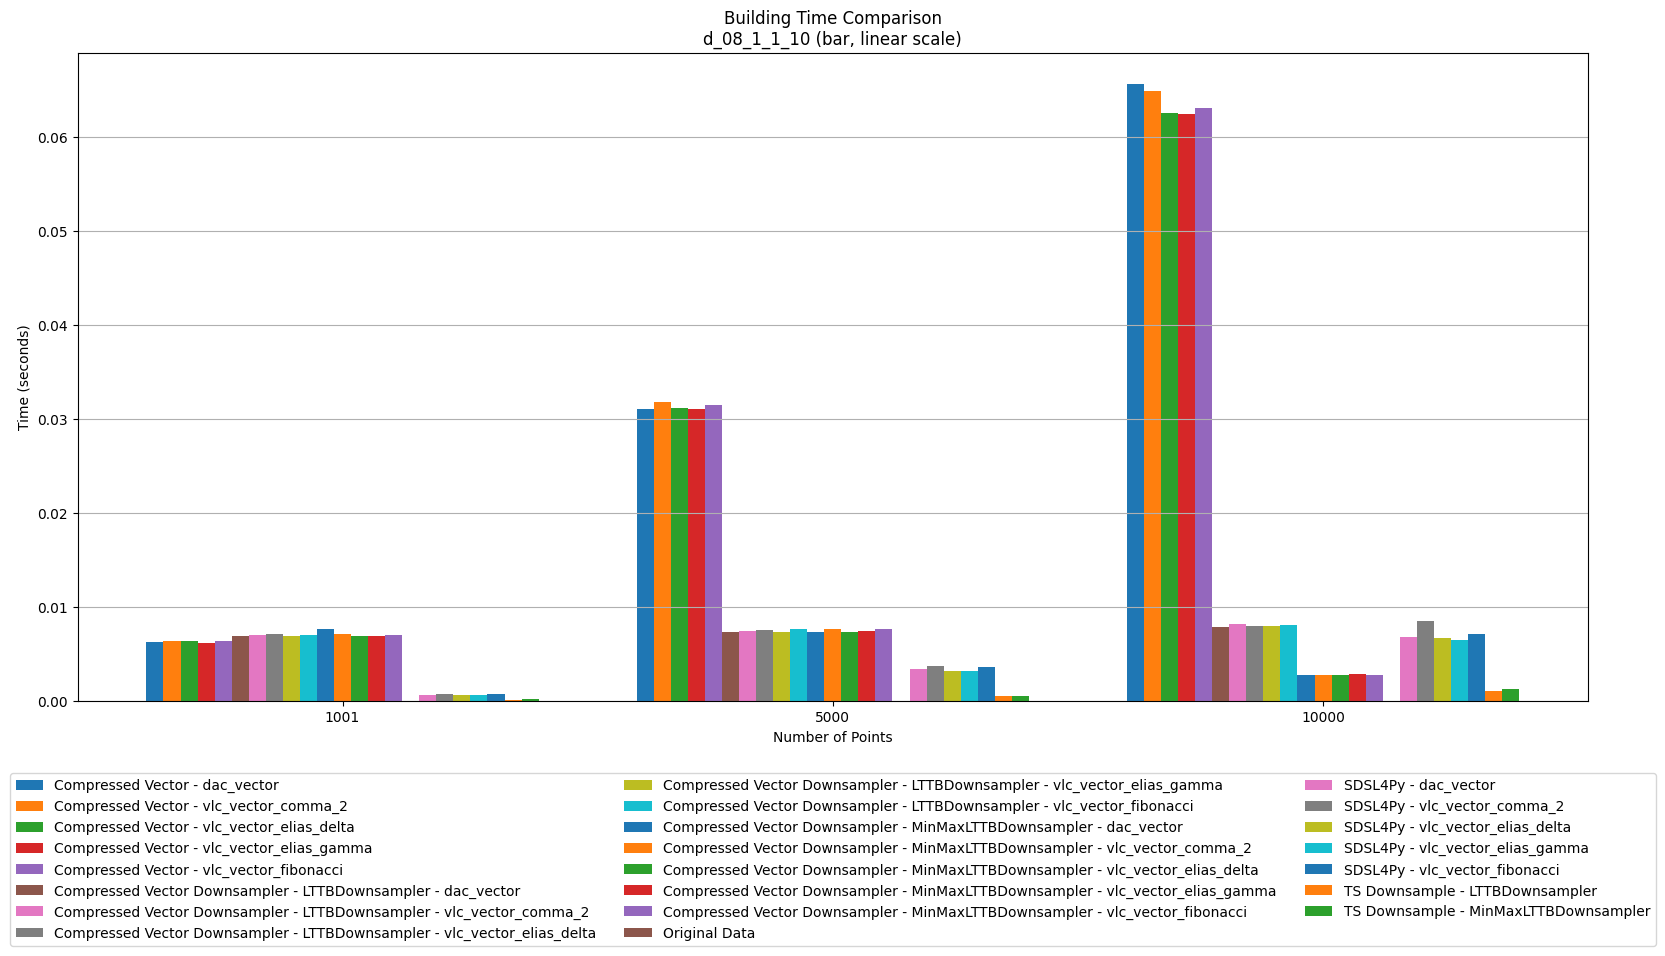
\includegraphics[width=1\textwidth]{anexo/exp/Building Time Comparison/bar_plots/Building Time Comparison_d_08_1_1_10_linear_bar.png}
        \caption[]{Gráfico de tiempo de construcción de las diferentes bibliotecas para el input \textbf{d\_08\_1\_1\_10}.}
        \label{fig:building_time_comparison_plot_bar_2}
    \end{figure}
}

\DeclareRobustCommand{\BuildingTimeComparisonThreePlotLine}{
    %insertar imagen
    \begin{figure}[H]
        \centering
        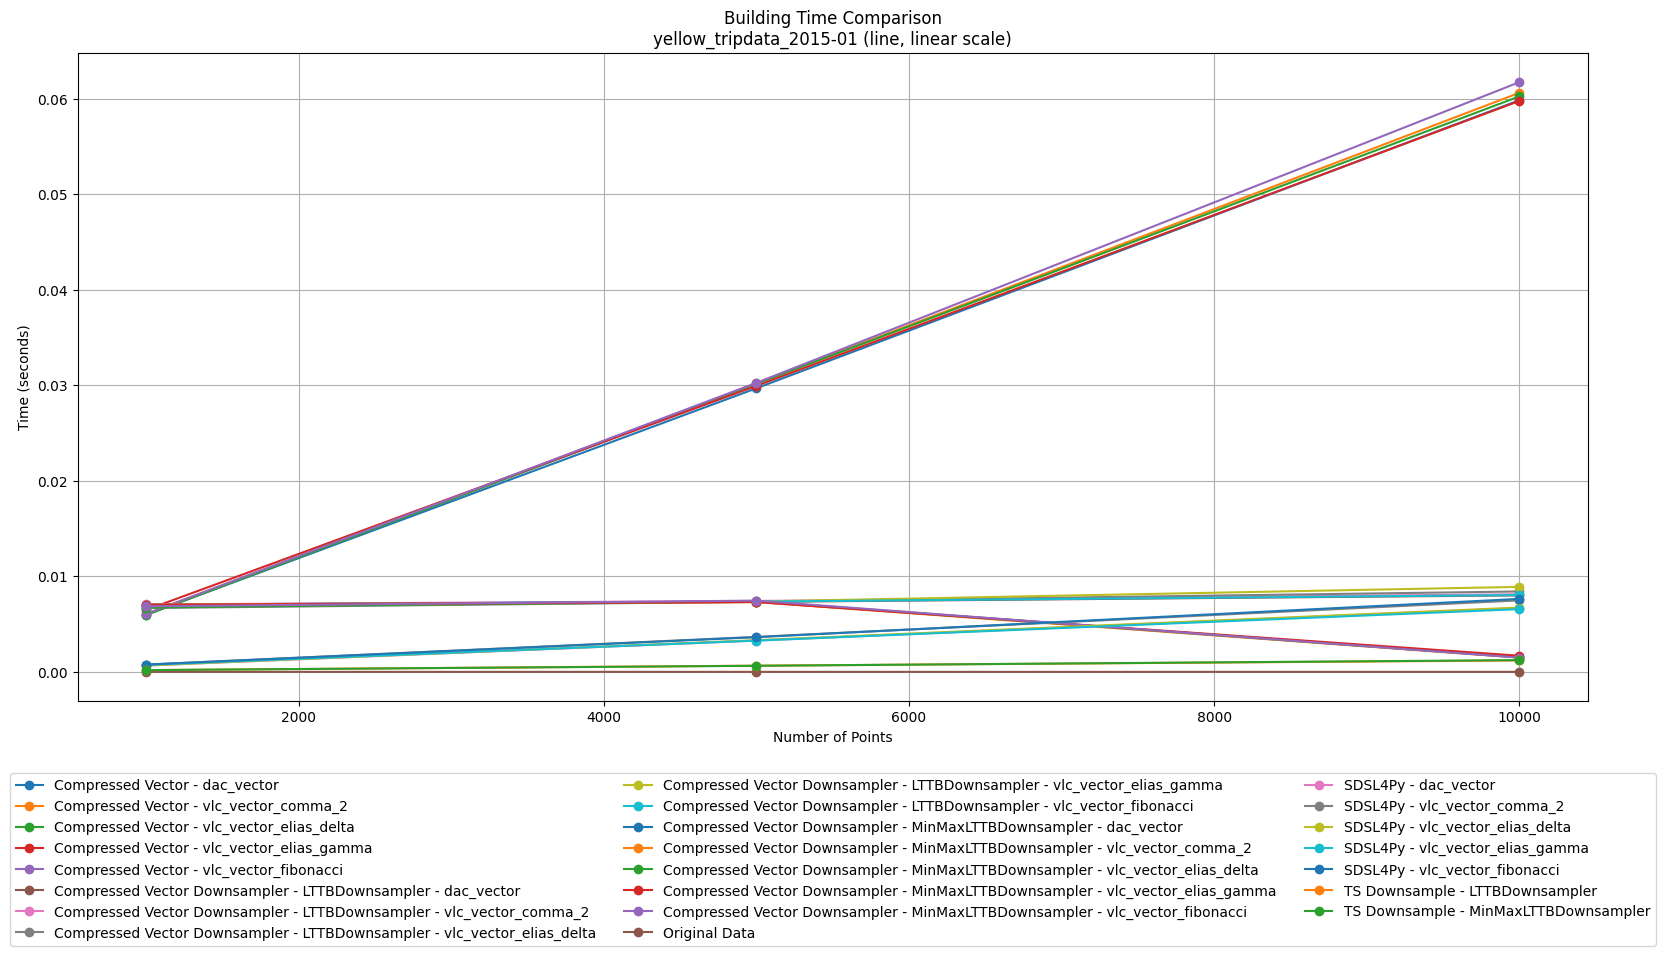
\includegraphics[width=1\textwidth]{anexo/exp/Building Time Comparison/plots/Building Time Comparison_yellow_tripdata_2015-01_linear_line.png}
        \caption[]{Gráfico de tiempo de construcción de las diferentes bibliotecas para el input \textbf{yellow\_tripdata\_2015\_01}.}
        \label{fig:building_time_comparison_plot_line_3}
    \end{figure}
}

\DeclareRobustCommand{\BuildingTimeComparisonThreePlotBar}{
    %insertar imagen
    \begin{figure}[H]
        \centering
        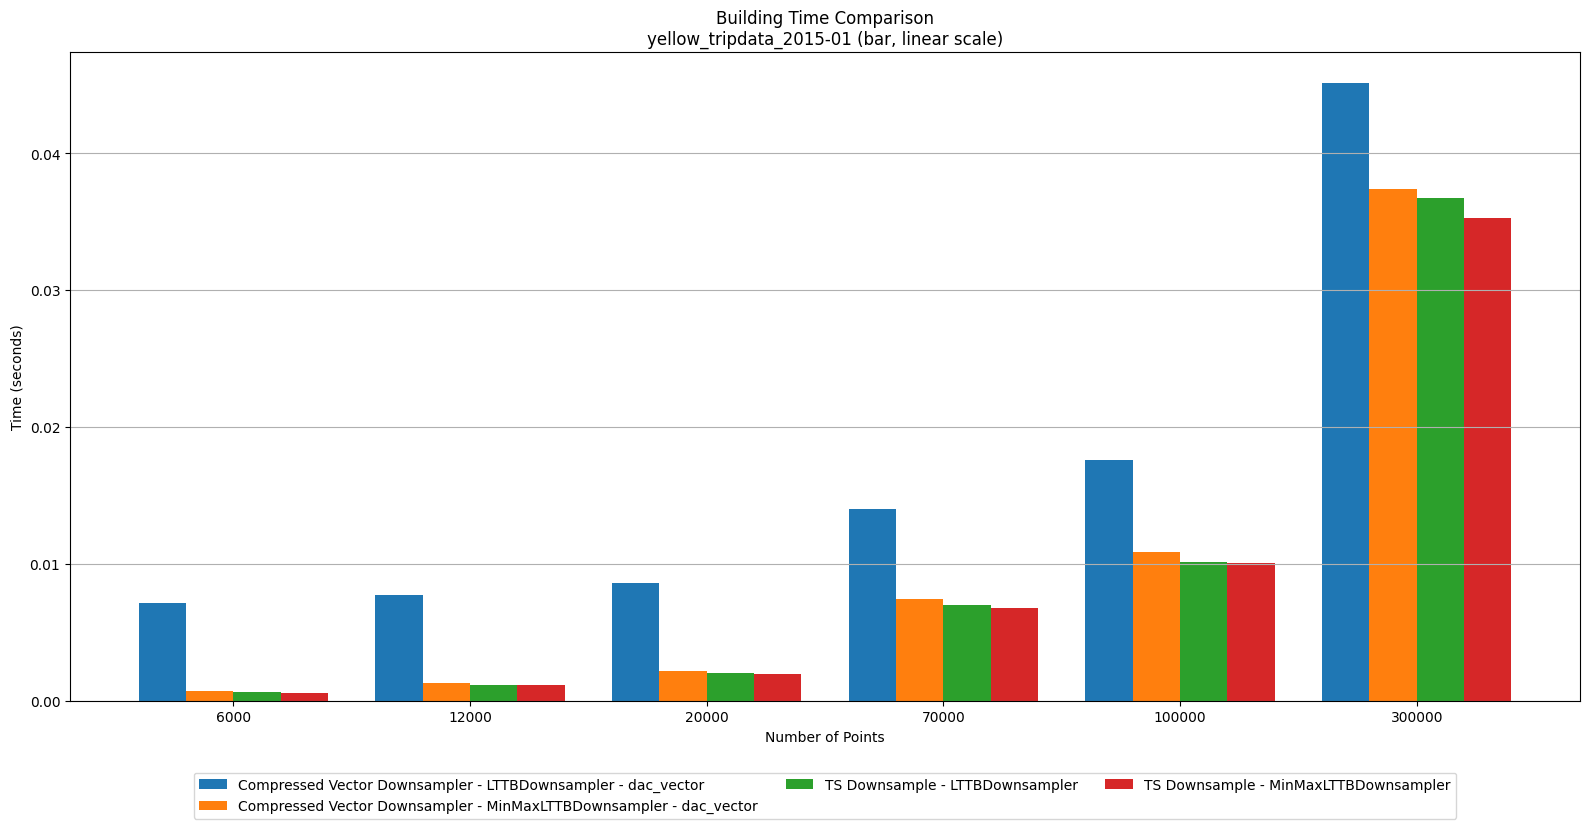
\includegraphics[width=1\textwidth]{anexo/exp/Building Time Comparison/bar_plots/Building Time Comparison_yellow_tripdata_2015-01_linear_bar.png}
        \caption[]{Gráfico de tiempo de construcción de las diferentes bibliotecas para el input \textbf{yellow\_tripdata\_2015\_01}.}
        \label{fig:building_time_comparison_plot_bar_3}
    \end{figure}
}




% Comparison of Space Used
\DeclareRobustCommand{\ComparisonOfSpaceUsedOnePlotLine}{
    %insertar imagen
    \begin{figure}[H]
        \centering
        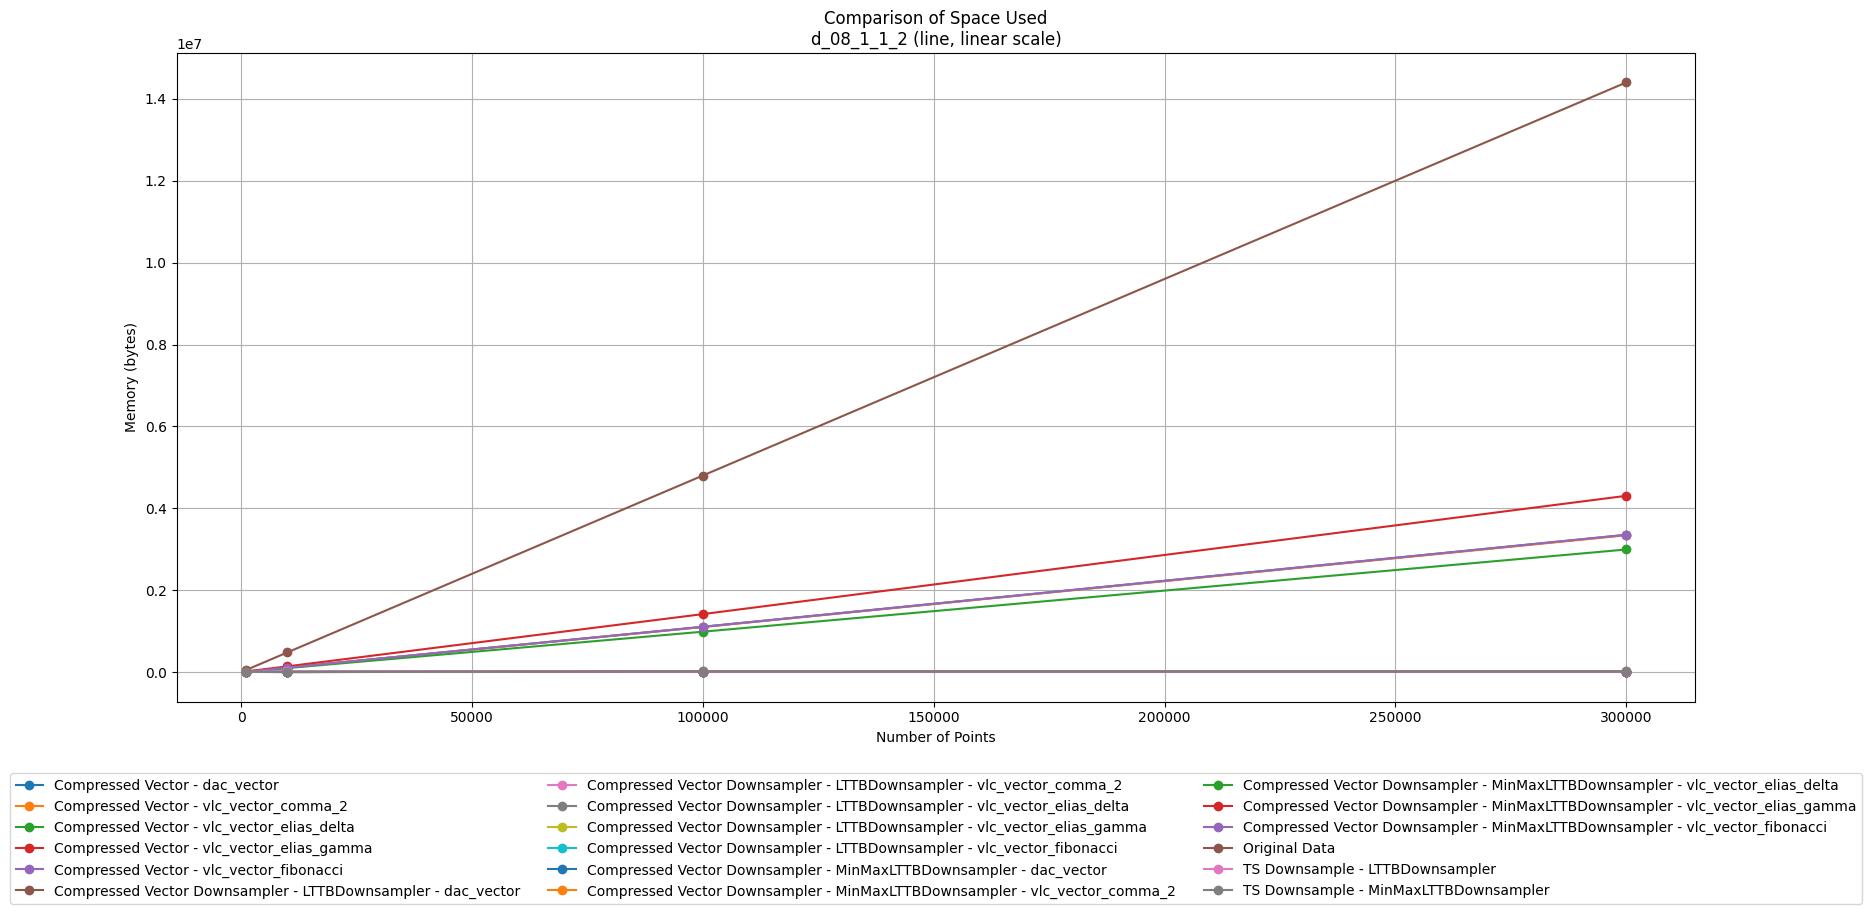
\includegraphics[width=1\textwidth]{anexo/exp/Comparison of Space Used/plots/Comparison of Space Used_d_08_1_1_2_linear_line.png}
        \caption[]{Gráfico de espacio usado por las diferentes bibliotecas para el input \textbf{d\_08\_1\_1\_2}.}
        \label{fig:comparison_of_space_used_plot_line_1}
    \end{figure}
}

\DeclareRobustCommand{\ComparisonOfSpaceUsedOnePlotBar}{
    %insertar imagen
    \begin{figure}[H]
        \centering
        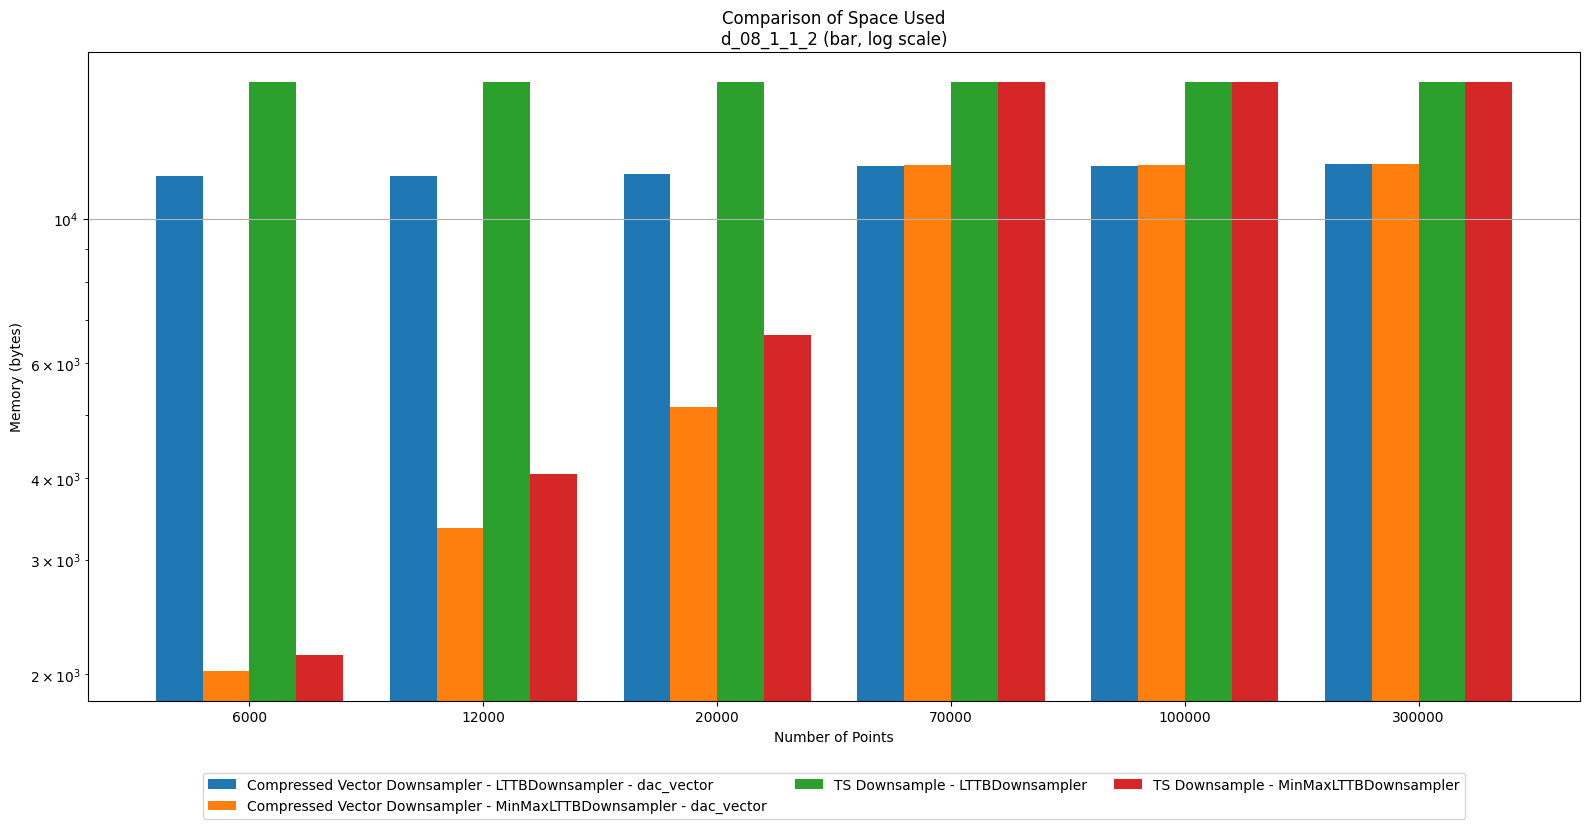
\includegraphics[width=1\textwidth]{anexo/exp/Comparison of Space Used/bar_plots/Comparison of Space Used_d_08_1_1_2_log_bar.png}
        \caption[]{Gráfico de espacio usado por las diferentes bibliotecas para el input \textbf{d\_08\_1\_1\_2}.}
        \label{fig:comparison_of_space_used_plot_bar_1}
    \end{figure}
    \begin{table}[H]
        \centering
        \resizebox{\textwidth}{!}{%
        \begin{tabular}{|l|c|c|c|c|c|c|}
        \hline\multicolumn{1}{|c|}{Option} & \multicolumn{6}{c|}{\textbf{Number of data points}} \\
        \cline{2-7}
         & \textbf{6000} & \textbf{12000} & \textbf{20000} & \textbf{70000} & \textbf{100000} & \textbf{300000} \\
        \hline
        Compressed Vector Downsample - dac\_vector & 1.66e+03 [B] & 2.68e+03 [B] & 4.07e+03 [B] & 9.49e+03 [B] & 9.48e+03 [B] & 9.54e+03 [B] \\
        Compressed Vector Downsample - vlc\_vector\_fibonacci & 1.24e+03 [B] & 2.26e+03 [B] & 3.65e+03 [B] & 8.89e+03 [B] & 8.88e+03 [B] & 9.04e+03 [B] \\
        Original Data & 1.06e+05 [B] & 2.16e+05 [B] & 3.46e+05 [B] & 1.12e+06 [B] & 1.60e+06 [B] & 5.20e+06 [B] \\
        TS Downsample & 2.14e+03 [B] & 4.06e+03 [B] & 6.62e+03 [B] & 1.62e+04 [B] & 1.62e+04 [B] & 1.62e+04 [B] \\
        \hline
        \end{tabular}
        }
        \label{tab:comparison of space used-d-08-1-1-2}
    \end{table}
    \begin{table}[H]
        \centering
        \caption{Comparison of Space Used\_d\_08\_1\_1\_2 – Tasa de compactación CVD vs TS vs Datos Originales}
        \label{tab:Comparison of Space Used\_d\_08\_1\_1\_2_cvd_compactacion}
        \begin{tabular}{rlrr}
        \toprule
        n\_size & Variante & Comp. vs TS (\%) & Comp. vs Original (\%) \\
        \midrule
        6000 & CVD - dac\_vector & 22.48 & 98.43 \\
        6000 & CVD - vlc\_vector\_fibonacci & 42.26 & 98.83 \\
        12000 & CVD - dac\_vector & 34.10 & 98.76 \\
        12000 & CVD - vlc\_vector\_fibonacci & 44.34 & 98.95 \\
        20000 & CVD - dac\_vector & 38.56 & 98.82 \\
        20000 & CVD - vlc\_vector\_fibonacci & 44.96 & 98.95 \\
        70000 & CVD - dac\_vector & 41.53 & 99.16 \\
        70000 & CVD - vlc\_vector\_fibonacci & 45.18 & 99.21 \\
        100000 & CVD - dac\_vector & 41.58 & 99.41 \\
        100000 & CVD - vlc\_vector\_fibonacci & 45.28 & 99.45 \\
        300000 & CVD - dac\_vector & 41.19 & 99.82 \\
        300000 & CVD - vlc\_vector\_fibonacci & 44.29 & 99.83 \\
        \bottomrule
        \end{tabular}
        
    \end{table}
}

\DeclareRobustCommand{\ComparisonOfSpaceUsedTwoPlotLine}{
    %insertar imagen
    \begin{figure}[H]
        \centering
        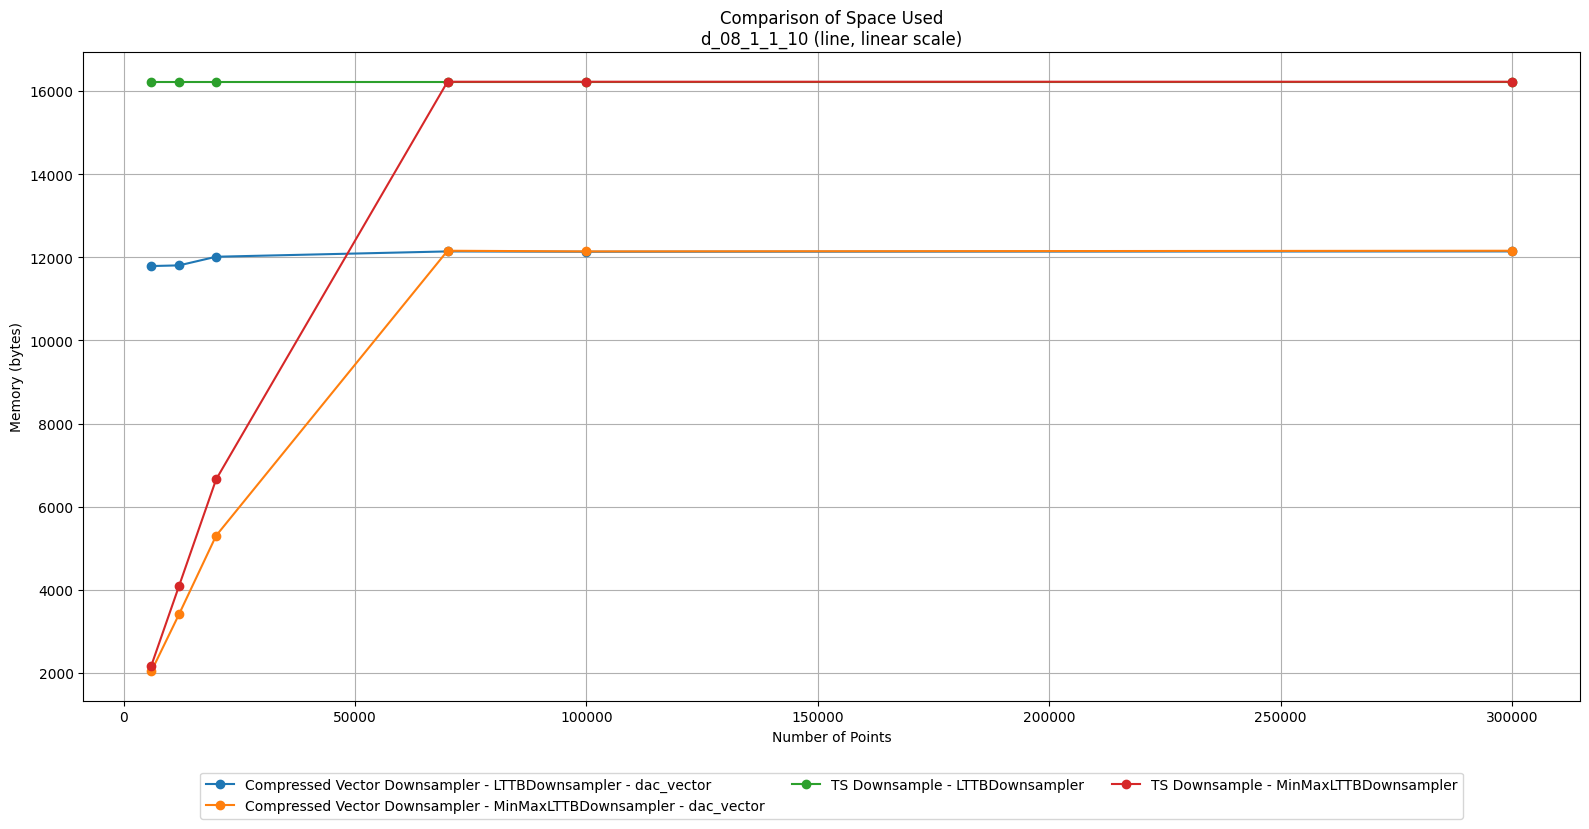
\includegraphics[width=1\textwidth]{anexo/exp/Comparison of Space Used/plots/Comparison of Space Used_d_08_1_1_10_linear_line.png}
        \caption[]{Gráfico de espacio usado por las diferentes bibliotecas para el input \textbf{d\_08\_1\_1\_10}.}
        \label{fig:comparison_of_space_used_plot_line_2}
    \end{figure}
}

\DeclareRobustCommand{\ComparisonOfSpaceUsedTwoPlotBar}{
    %insertar imagen
    \begin{figure}[H]
        \centering
        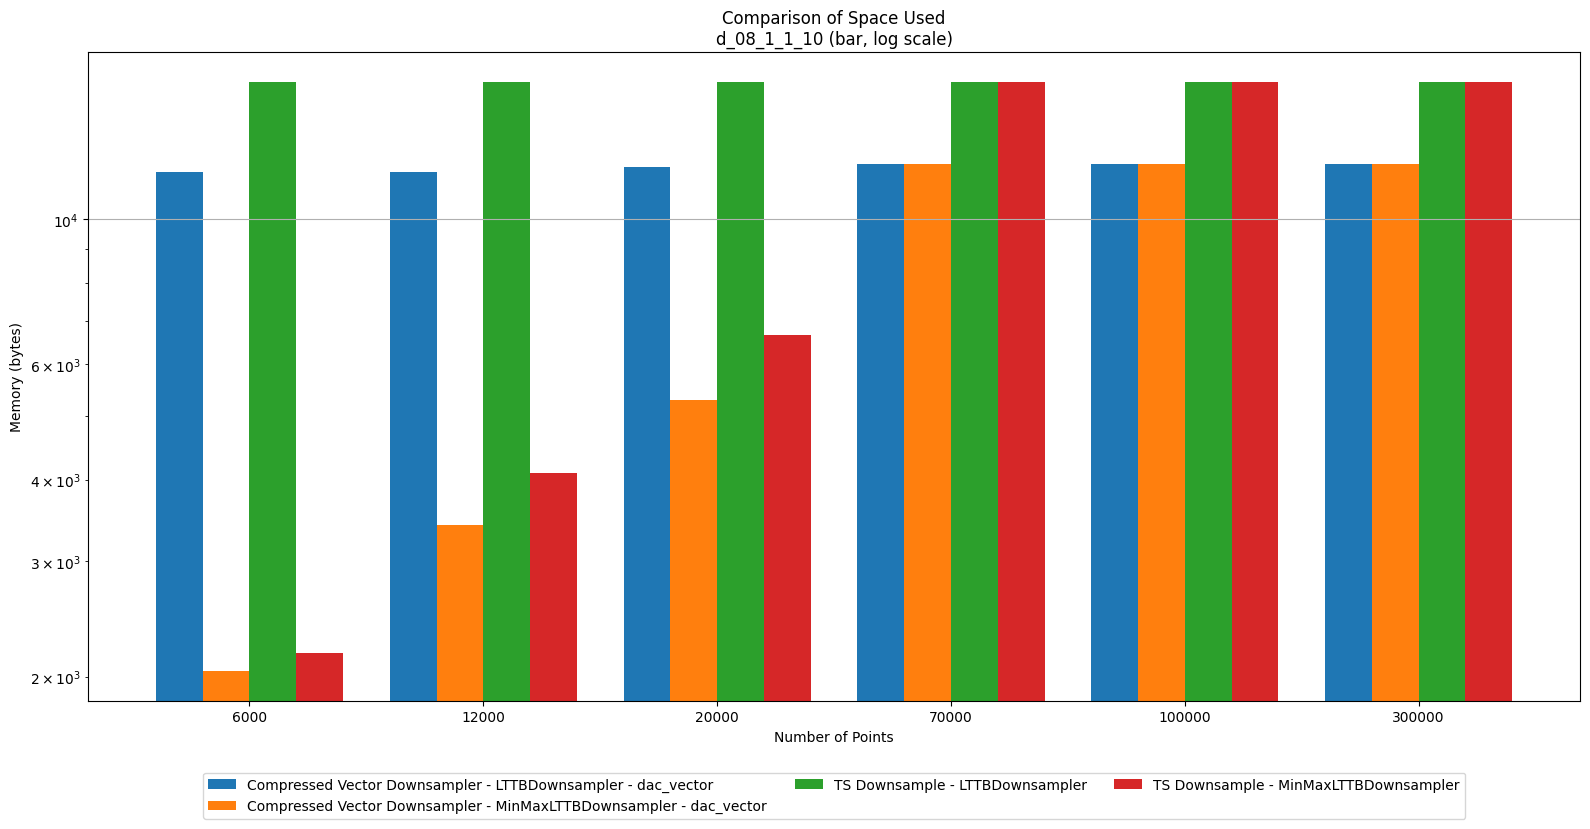
\includegraphics[width=1\textwidth]{anexo/exp/Comparison of Space Used/bar_plots/Comparison of Space Used_d_08_1_1_10_log_bar.png}
        \caption[]{Gráfico de espacio usado por las diferentes bibliotecas para el input \textbf{d\_08\_1\_1\_10}.}
        \label{fig:comparison_of_space_used_plot_bar_2}
    \end{figure}

    \begin{table}[H]
        \centering
        \resizebox{\textwidth}{!}{%
        \begin{tabular}{|l|c|c|c|c|c|c|}
        \hline\multicolumn{1}{|c|}{Option} & \multicolumn{6}{c|}{\textbf{Number of data points}} \\
        \cline{2-7}
         & \textbf{6000} & \textbf{12000} & \textbf{20000} & \textbf{70000} & \textbf{100000} & \textbf{300000} \\
        \hline
        Compressed Vector Downsample - dac\_vector & 1.67e+03 [B] & 2.73e+03 [B] & 4.21e+03 [B] & 9.57e+03 [B] & 9.55e+03 [B] & 9.57e+03 [B] \\
        Compressed Vector Downsample - vlc\_vector\_fibonacci & 1.28e+03 [B] & 2.33e+03 [B] & 3.77e+03 [B] & 9.15e+03 [B] & 9.13e+03 [B] & 9.17e+03 [B] \\
        Original Data & 1.06e+05 [B] & 2.16e+05 [B] & 3.46e+05 [B] & 1.12e+06 [B] & 1.60e+06 [B] & 5.20e+06 [B] \\
        TS Downsample & 2.18e+03 [B] & 4.10e+03 [B] & 6.66e+03 [B] & 1.62e+04 [B] & 1.62e+04 [B] & 1.62e+04 [B] \\
        \hline
        \end{tabular}
        }
        \label{tab:comparison of space used-d-08-1-1-10}
    \end{table}
        \begin{table}[H]
\centering
\caption{Comparison of Space Used\_d\_08\_1\_1\_10 – Tasa de compactación CVD vs TS vs Datos Originales}
\label{tab:Comparison of Space Used\_d\_08\_1\_1\_10_cvd_compactacion}
\begin{tabular}{rlrr}
\toprule
n\_size & Variante & Comp. vs TS (\%) & Comp. vs Original (\%) \\
\midrule
6000 & CVD - dac\_vector & 23.25 & 98.43 \\
6000 & CVD - vlc\_vector\_fibonacci & 41.27 & 98.80 \\
12000 & CVD - dac\_vector & 33.45 & 98.74 \\
12000 & CVD - vlc\_vector\_fibonacci & 43.02 & 98.92 \\
20000 & CVD - dac\_vector & 36.81 & 98.78 \\
20000 & CVD - vlc\_vector\_fibonacci & 43.42 & 98.91 \\
70000 & CVD - dac\_vector & 41.04 & 99.15 \\
70000 & CVD - vlc\_vector\_fibonacci & 43.60 & 99.19 \\
100000 & CVD - dac\_vector & 41.14 & 99.40 \\
100000 & CVD - vlc\_vector\_fibonacci & 43.75 & 99.43 \\
300000 & CVD - dac\_vector & 41.04 & 99.82 \\
300000 & CVD - vlc\_vector\_fibonacci & 43.45 & 99.82 \\
\bottomrule
\end{tabular}

\end{table}
}

\DeclareRobustCommand{\ComparisonOfSpaceUsedThreePlotLine}{
    %insertar imagen
    \begin{figure}[H]
        \centering
        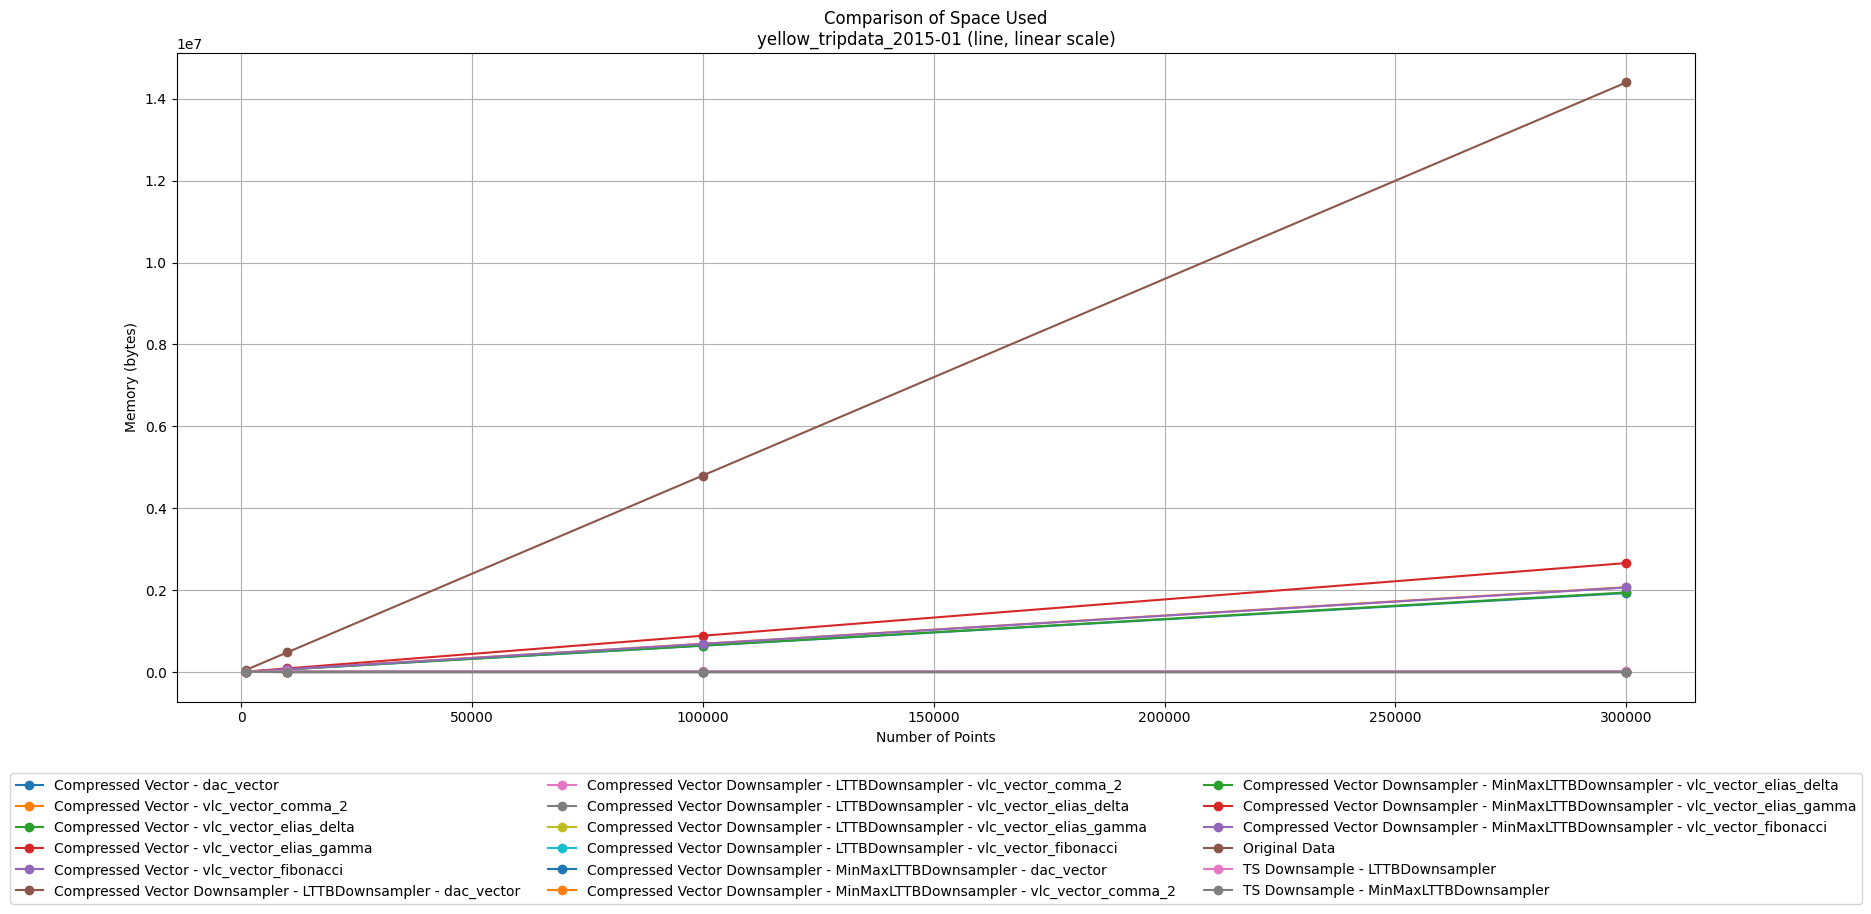
\includegraphics[width=1\textwidth]{anexo/exp/Comparison of Space Used/plots/Comparison of Space Used_yellow_tripdata_2015-01_linear_line.png}
        \caption[]{Gráfico de espacio usado por las diferentes bibliotecas para el input \textbf{yellow\_tripdata\_2015\_01}.}
        \label{fig:comparison_of_space_used_plot_line_3}
    \end{figure}
}

\DeclareRobustCommand{\ComparisonOfSpaceUsedThreePlotBar}{
    %insertar imagen
    \begin{figure}[H]
        \centering
        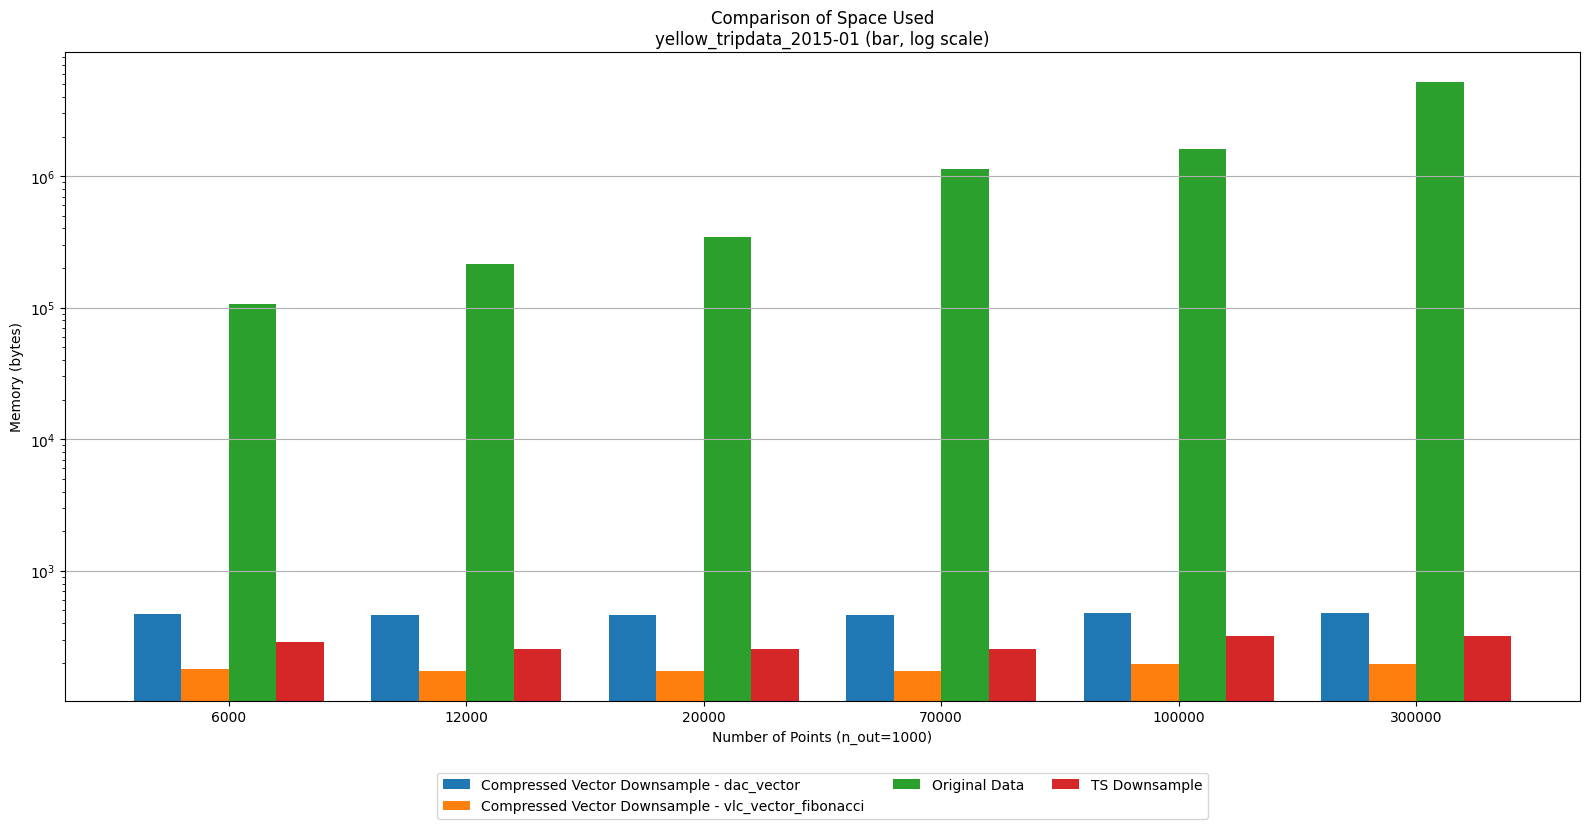
\includegraphics[width=1\textwidth]{anexo/exp/Comparison of Space Used/bar_plots/Comparison of Space Used_yellow_tripdata_2015-01_log_bar.png}
        \caption[]{Gráfico de espacio usado por las diferentes bibliotecas para el input \textbf{yellow\_tripdata\_2015\_01}.}
        \label{fig:comparison_of_space_used_plot_bar_3}
    \end{figure}
    \begin{table}[H]
        \centering
        \resizebox{\textwidth}{!}{%
        \begin{tabular}{|l|c|c|c|c|c|c|}
        \hline\multicolumn{1}{|c|}{Option} & \multicolumn{6}{c|}{\textbf{Number of data points}} \\
        \cline{2-7}
         & \textbf{6000} & \textbf{12000} & \textbf{20000} & \textbf{70000} & \textbf{100000} & \textbf{300000} \\
        \hline
        Compressed Vector Downsample - dac\_vector & 4.68e+02 [B] & 4.60e+02 [B] & 4.60e+02 [B] & 4.60e+02 [B] & 4.76e+02 [B] & 4.76e+02 [B] \\
        Compressed Vector Downsample - vlc\_vector\_fibonacci & 1.80e+02 [B] & 1.72e+02 [B] & 1.72e+02 [B] & 1.72e+02 [B] & 1.96e+02 [B] & 1.96e+02 [B] \\
        Original Data & 1.06e+05 [B] & 2.16e+05 [B] & 3.46e+05 [B] & 1.12e+06 [B] & 1.60e+06 [B] & 5.20e+06 [B] \\
        TS Downsample & 2.88e+02 [B] & 2.56e+02 [B] & 2.56e+02 [B] & 2.56e+02 [B] & 3.20e+02 [B] & 3.20e+02 [B] \\
        \hline
        \end{tabular}
        }
        \label{tab:comparison of space used-yellow-tripdata-2015-01}
    \end{table}
    \begin{table}[H]
\centering
\caption{Comparison of Space Used\_yellow\_tripdata\_2015-01 – Tasa de compactación CVD vs TS vs Datos Originales}
\label{tab:Comparison of Space Used\_yellow\_tripdata\_2015-01_cvd_compactacion}
\begin{tabular}{rlrr}
\toprule
n\_size & Variante & Comp. vs TS (\%) & Comp. vs Original (\%) \\
\midrule
6000 & CVD - dac\_vector & -62.50 & 99.56 \\
6000 & CVD - vlc\_vector\_fibonacci & 37.50 & 99.83 \\
12000 & CVD - dac\_vector & -79.69 & 99.79 \\
12000 & CVD - vlc\_vector\_fibonacci & 32.81 & 99.92 \\
20000 & CVD - dac\_vector & -79.69 & 99.87 \\
20000 & CVD - vlc\_vector\_fibonacci & 32.81 & 99.95 \\
70000 & CVD - dac\_vector & -79.69 & 99.96 \\
70000 & CVD - vlc\_vector\_fibonacci & 32.81 & 99.98 \\
100000 & CVD - dac\_vector & -48.75 & 99.97 \\
100000 & CVD - vlc\_vector\_fibonacci & 38.75 & 99.99 \\
300000 & CVD - dac\_vector & -48.75 & 99.99 \\
300000 & CVD - vlc\_vector\_fibonacci & 38.75 & 100.00 \\
\bottomrule
\end{tabular}

\end{table}
}



% ===========================
% CVD Decimal Places Access Time Comparison
% ===========================
\DeclareRobustCommand{\CVDDecimalPlacesAccessTimeComparisonOnePlotLine}{
    \begin{figure}[H]
        \centering
        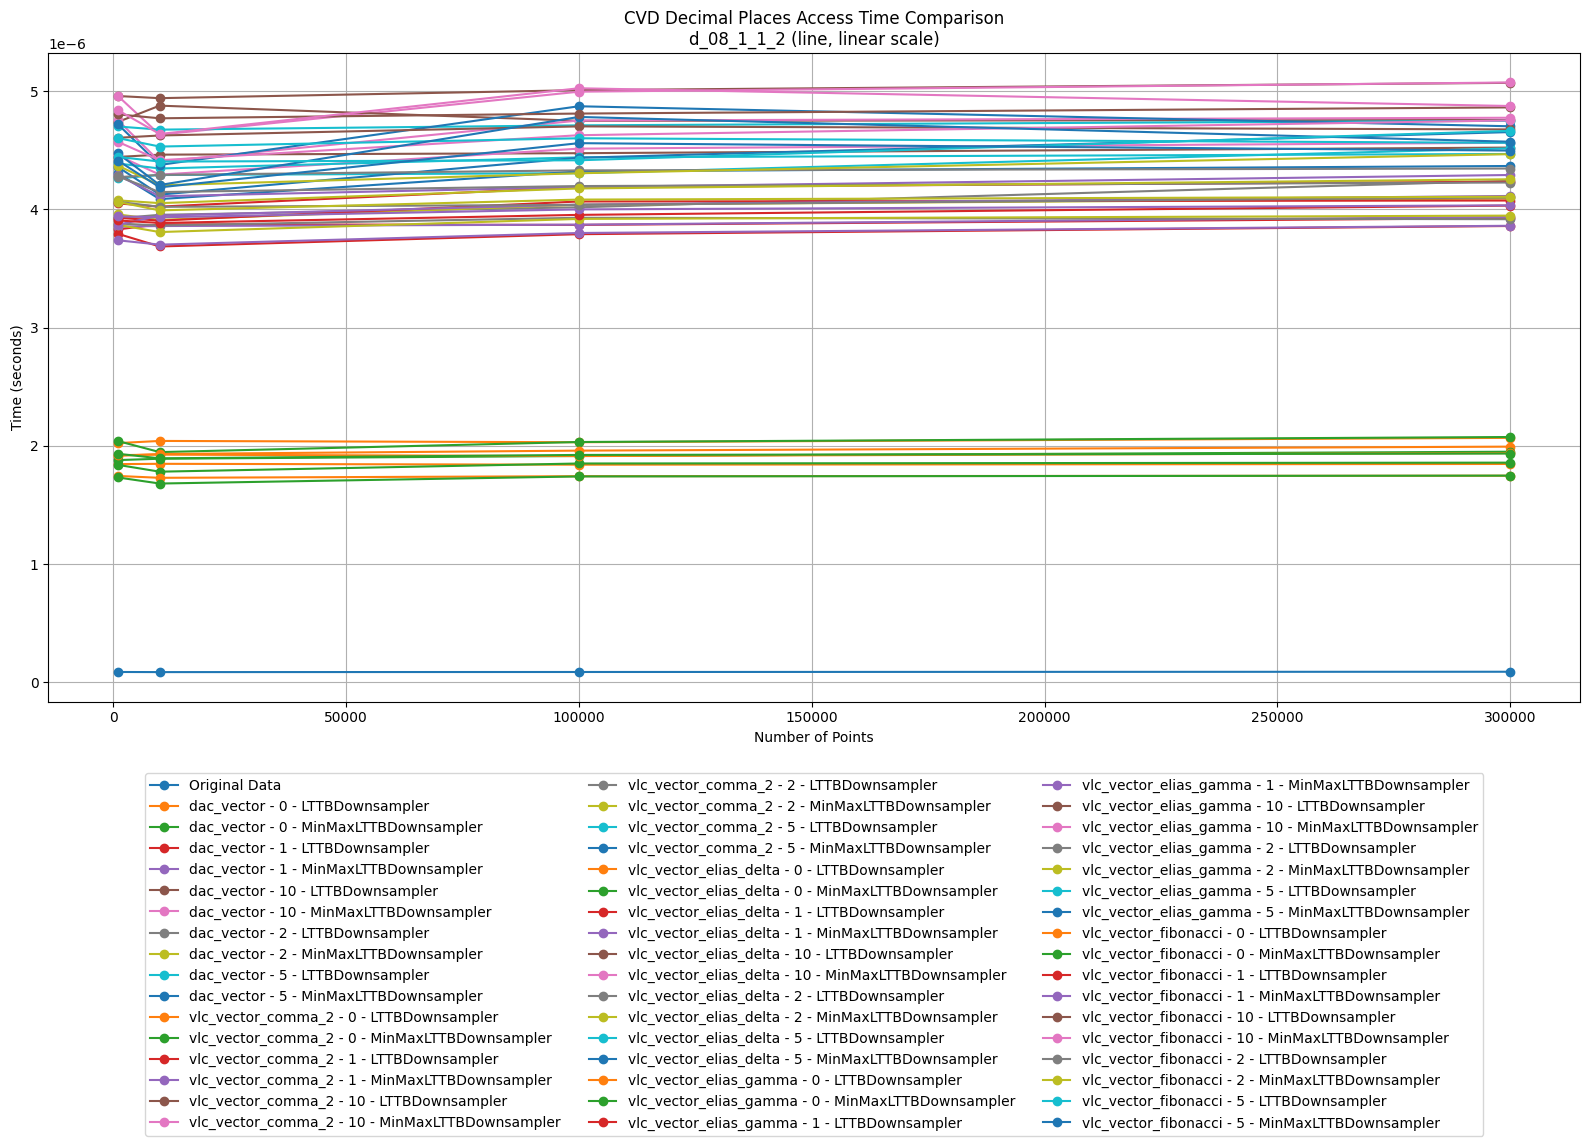
\includegraphics[width=1\textwidth]{anexo/exp/CVD Decimal Places Access Time Comparison/plots/CVD Decimal Places Access Time Comparison_d_08_1_1_2_linear_line.png}
        \caption[]{Gráfico de tiempo de acceso CVD con diferentes lugares decimales para el input \textbf{d\_08\_1\_1\_2}.}
        \label{fig:cvd_decimal_places_access_time_comparison_plot_line_1}
    \end{figure}
    \begin{figure}[H]
        \centering
        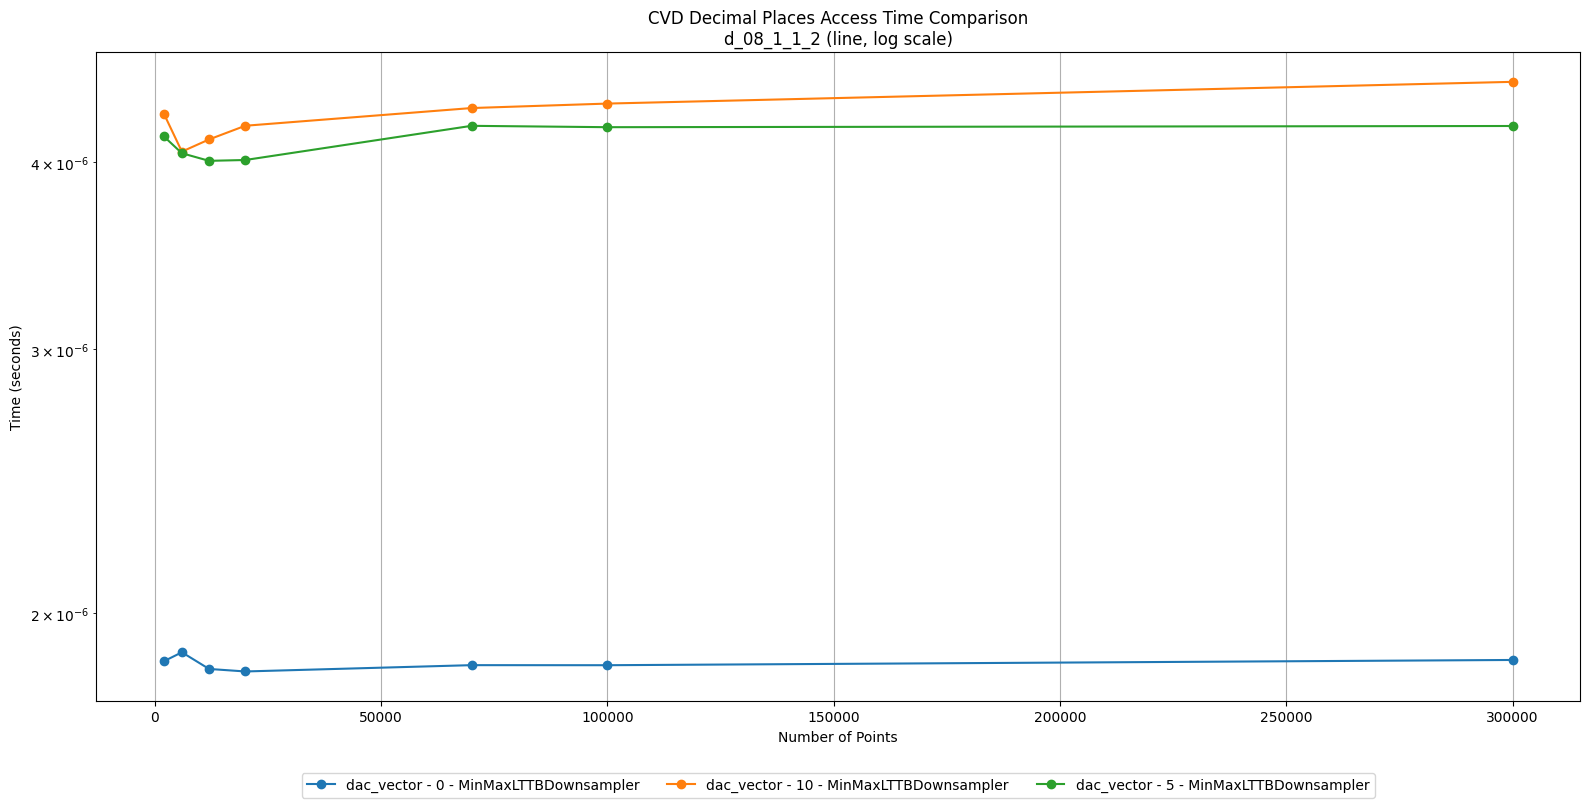
\includegraphics[width=1\textwidth]{anexo/exp/CVD Decimal Places Access Time Comparison/plots/CVD Decimal Places Access Time Comparison_d_08_1_1_2_log_line.png}
        \caption[]{Gráfico de tiempo de acceso CVD con diferentes lugares decimales para el input \textbf{d\_08\_1\_1\_2} en escala logarítmica.}
        \label{fig:cvd_decimal_places_access_time_comparison_plot_log_1}
    \end{figure}
}

\DeclareRobustCommand{\CVDDecimalPlacesAccessTimeComparisonTwoPlotLine}{
    \begin{figure}[H]
        \centering
        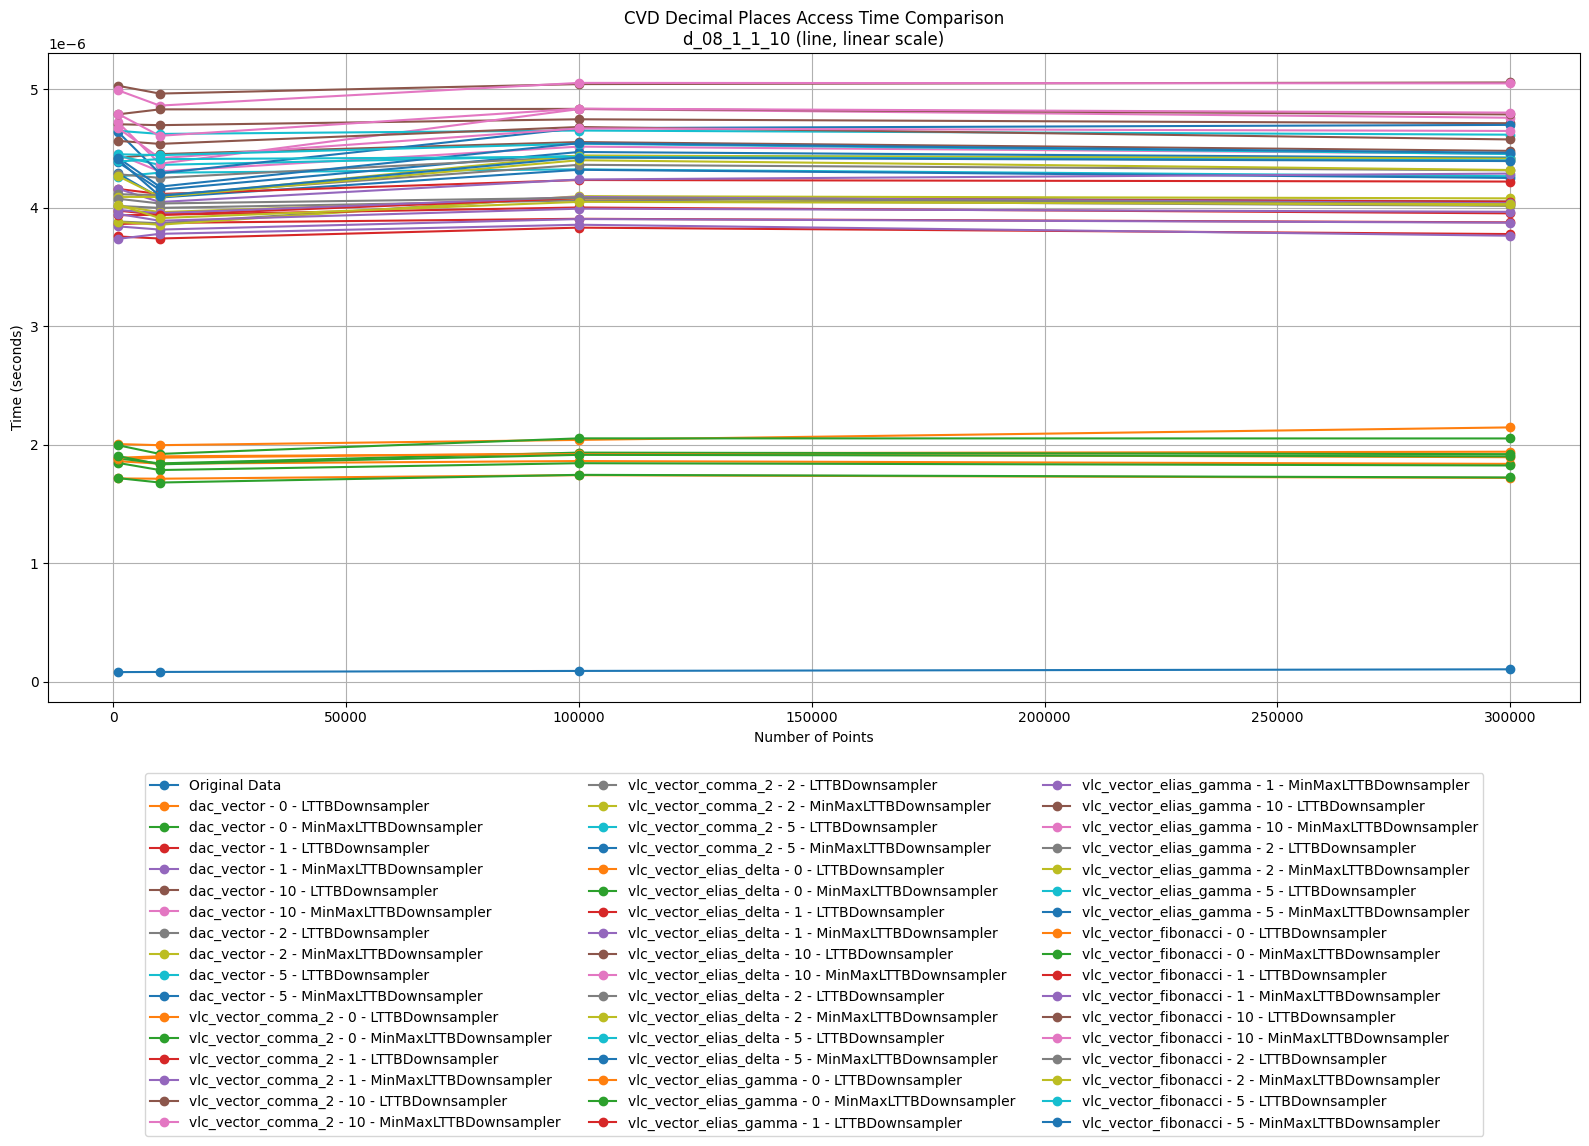
\includegraphics[width=1\textwidth]{anexo/exp/CVD Decimal Places Access Time Comparison/plots/CVD Decimal Places Access Time Comparison_d_08_1_1_10_linear_line.png}
        \caption[]{Gráfico de tiempo de acceso CVD con diferentes lugares decimales para el input \textbf{d\_08\_1\_1\_10}.}
        \label{fig:cvd_decimal_places_access_time_comparison_plot_line_2}
    \end{figure}
    \begin{figure}[H]
        \centering
        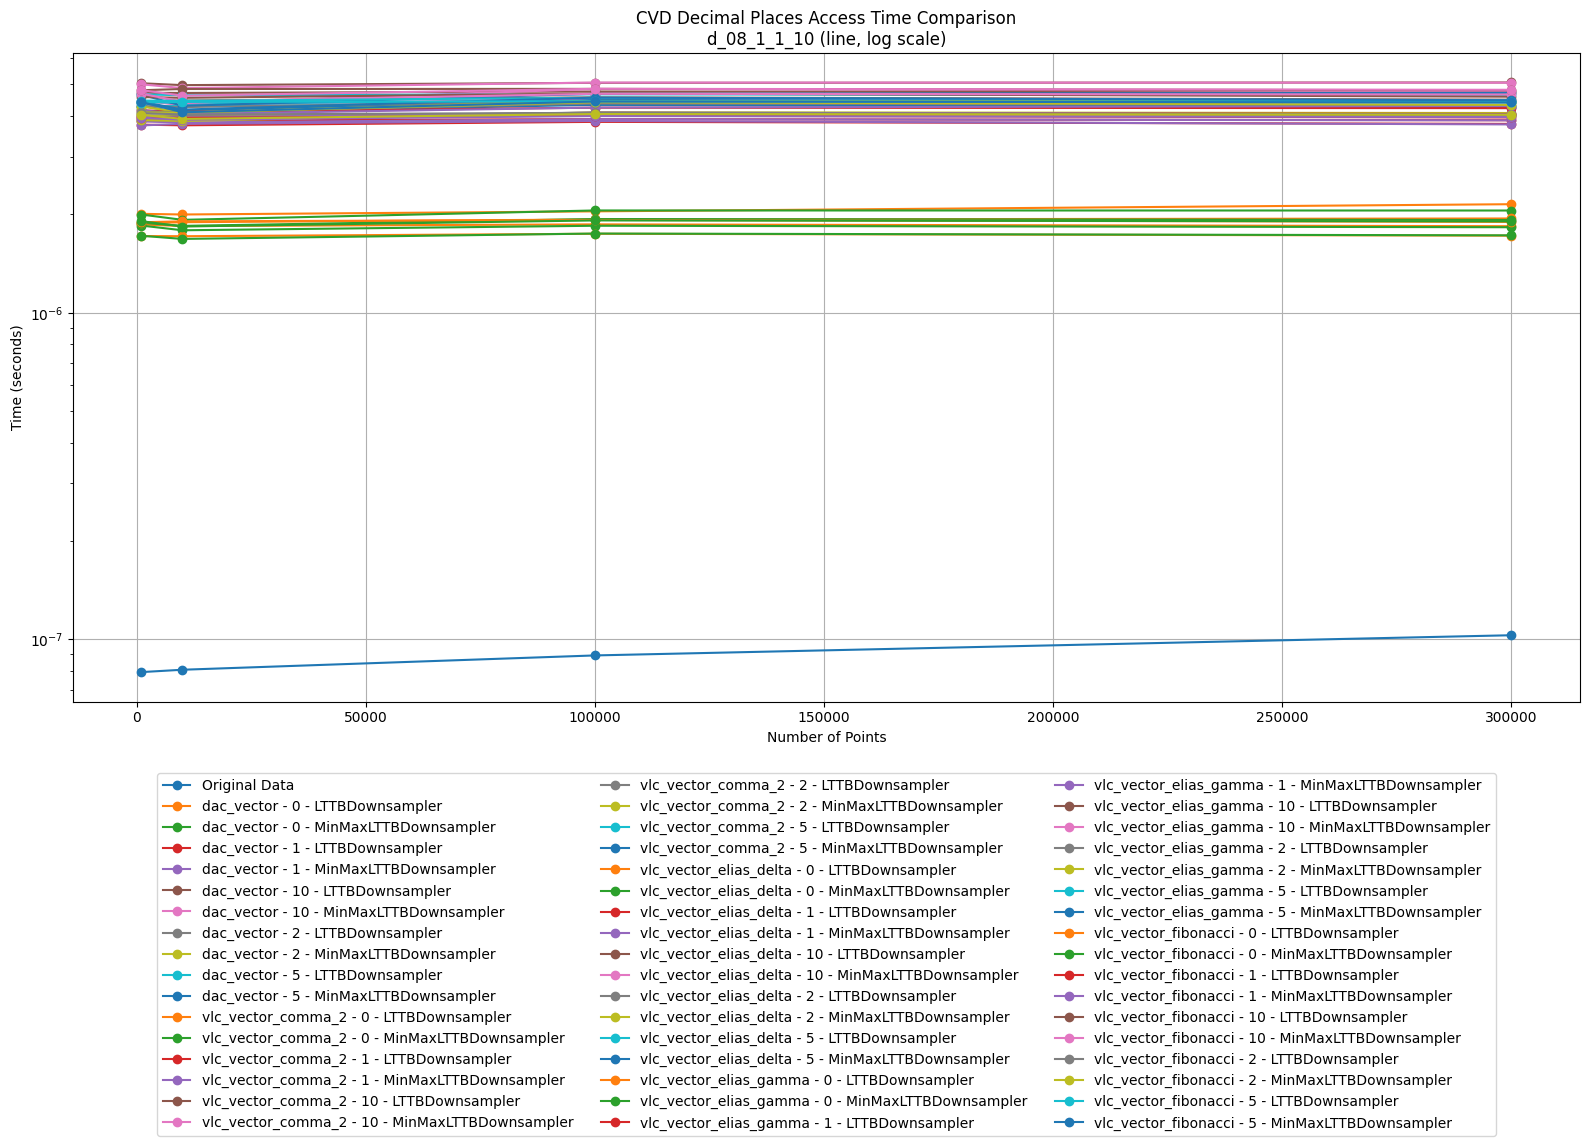
\includegraphics[width=1\textwidth]{anexo/exp/CVD Decimal Places Access Time Comparison/plots/CVD Decimal Places Access Time Comparison_d_08_1_1_10_log_line.png}
        \caption[]{Gráfico de tiempo de acceso CVD con diferentes lugares decimales para el input \textbf{d\_08\_1\_1\_10} en escala logarítmica.}
        \label{fig:cvd_decimal_places_access_time_comparison_plot_log_2}
    \end{figure}
}

\DeclareRobustCommand{\CVDDecimalPlacesAccessTimeComparisonThreePlotLine}{
    \begin{figure}[H]
        \centering
        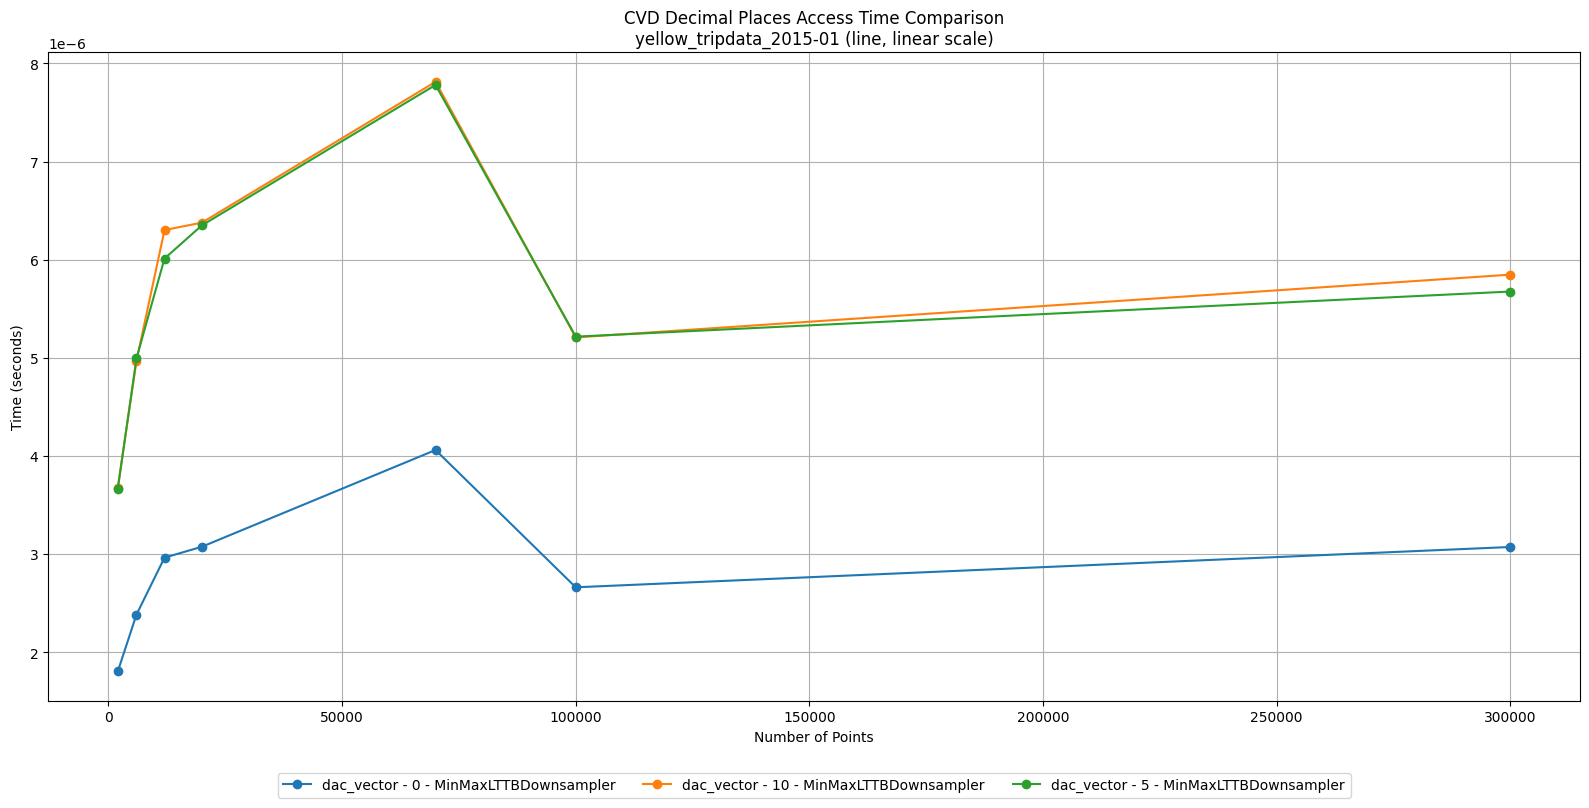
\includegraphics[width=1\textwidth]{anexo/exp/CVD Decimal Places Access Time Comparison/plots/CVD Decimal Places Access Time Comparison_yellow_tripdata_2015-01_linear_line.png}
        \caption[]{Gráfico de tiempo de acceso CVD con diferentes lugares decimales para el input \textbf{yellow\_tripdata\_2015\_01}.}
        \label{fig:cvd_decimal_places_access_time_comparison_plot_line_3}
    \end{figure}
    \begin{figure}[H]
        \centering
        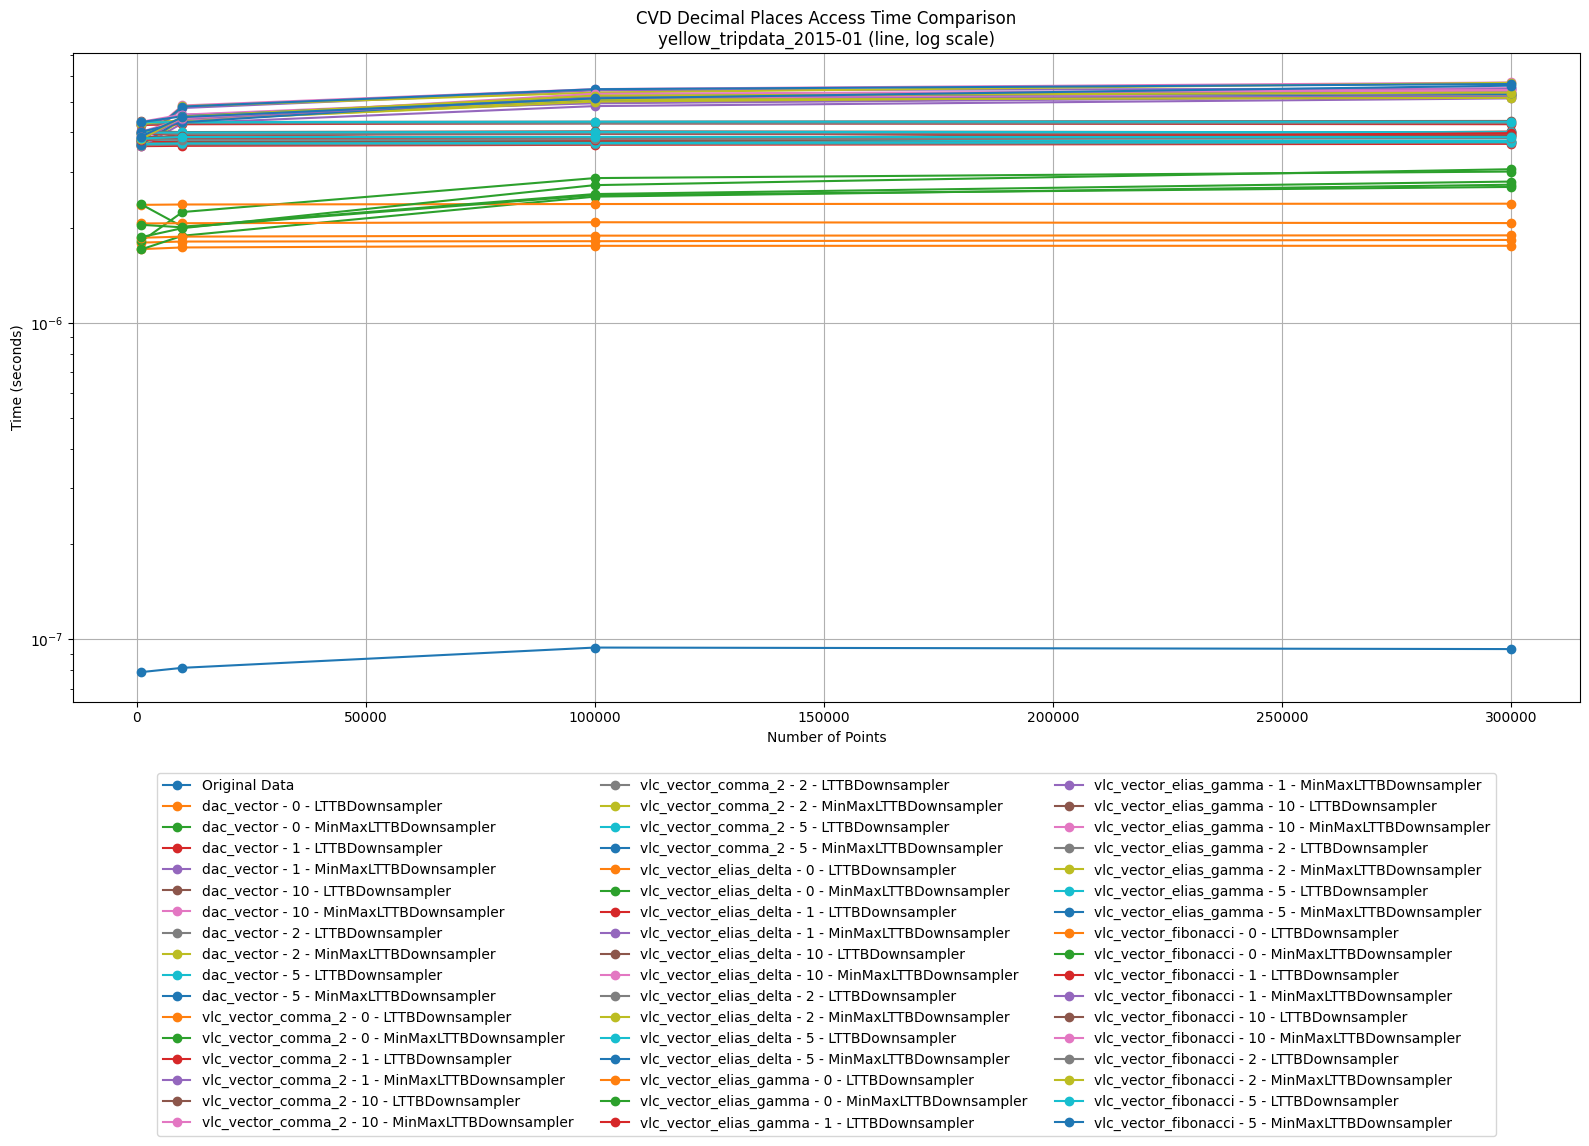
\includegraphics[width=1\textwidth]{anexo/exp/CVD Decimal Places Access Time Comparison/plots/CVD Decimal Places Access Time Comparison_yellow_tripdata_2015-01_log_line.png}
        \caption[]{Gráfico de tiempo de acceso CVD con diferentes lugares decimales para el input \textbf{yellow\_tripdata\_2015\_01} en escala logarítmica.}
        \label{fig:cvd_decimal_places_access_time_comparison_plot_log_3}
    \end{figure}
}


% ===========================
% CVD Decimal Places Build Time Comparison
% ===========================
\DeclareRobustCommand{\CVDDecimalPlacesBuildTimeComparisonOnePlotLine}{
    \begin{figure}[H]
        \centering
        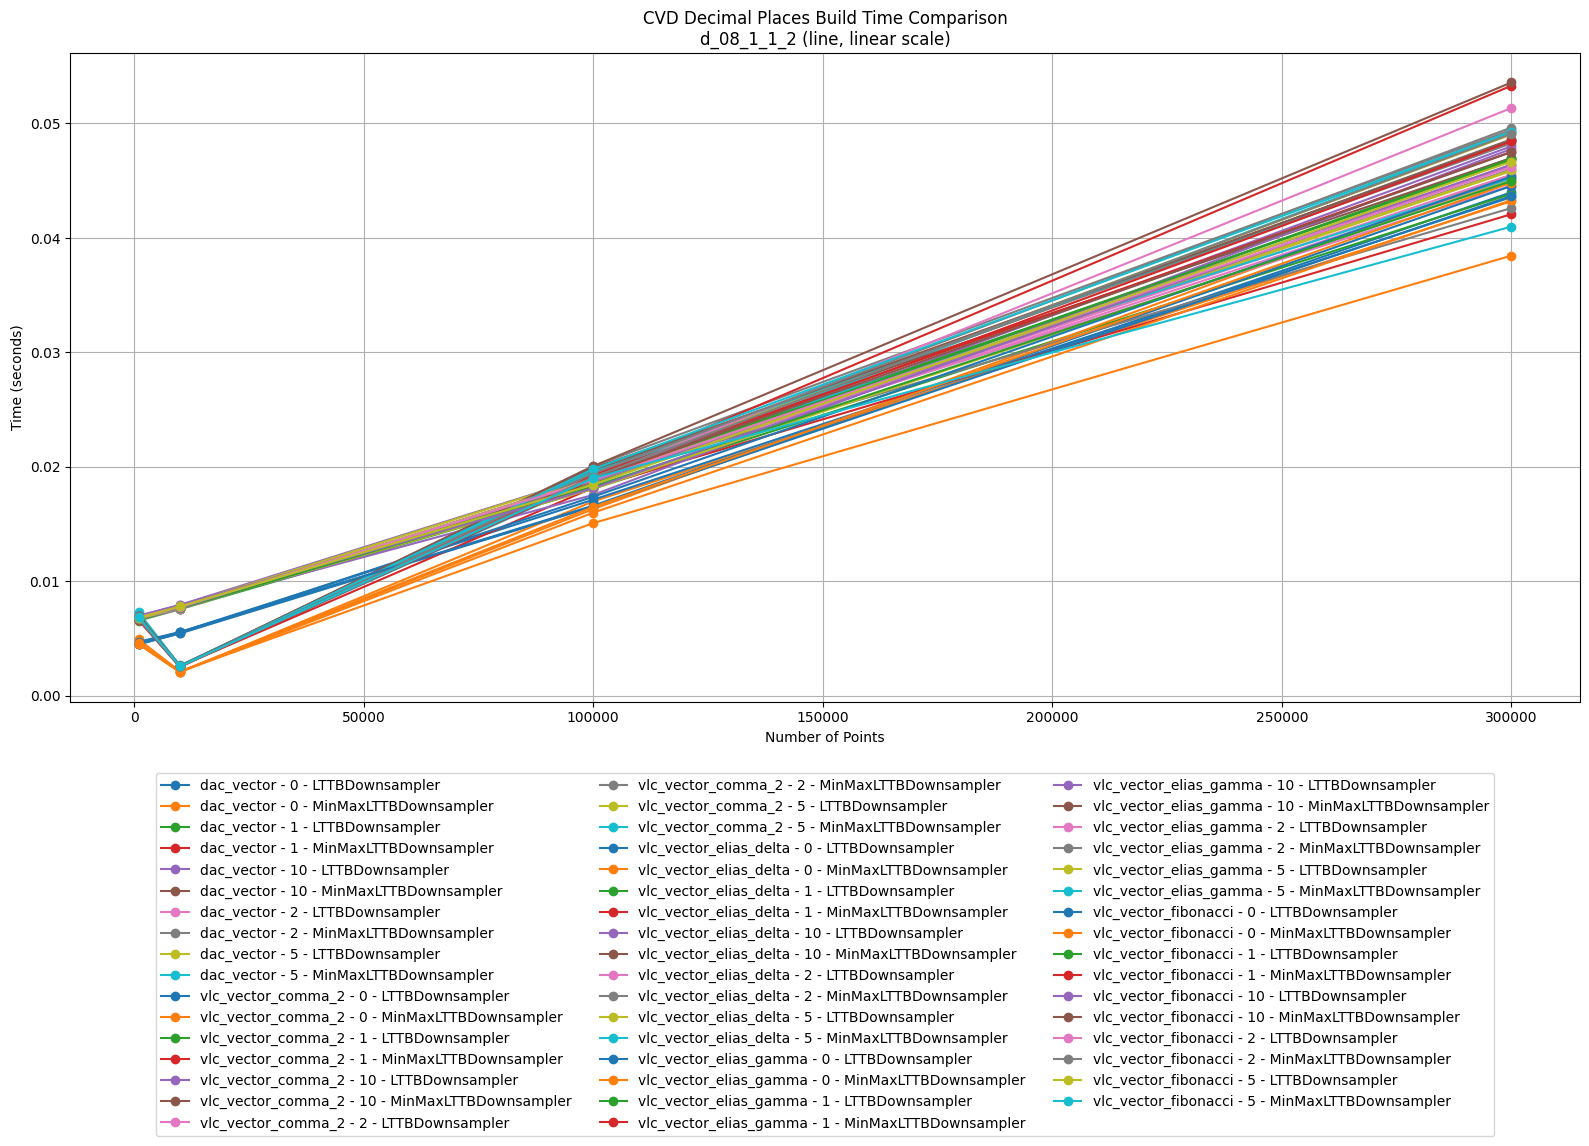
\includegraphics[width=1\textwidth]{anexo/exp/CVD Decimal Places Build Time Comparison/plots/CVD Decimal Places Build Time Comparison_d_08_1_1_2_linear_line.png}
        \caption[]{Gráfico de tiempo de construcción CVD con diferentes lugares decimales para el input \textbf{d\_08\_1\_1\_2}.}
        \label{fig:cvd_decimal_places_build_time_comparison_plot_line_1}
    \end{figure}
    \begin{figure}[H]
        \centering
        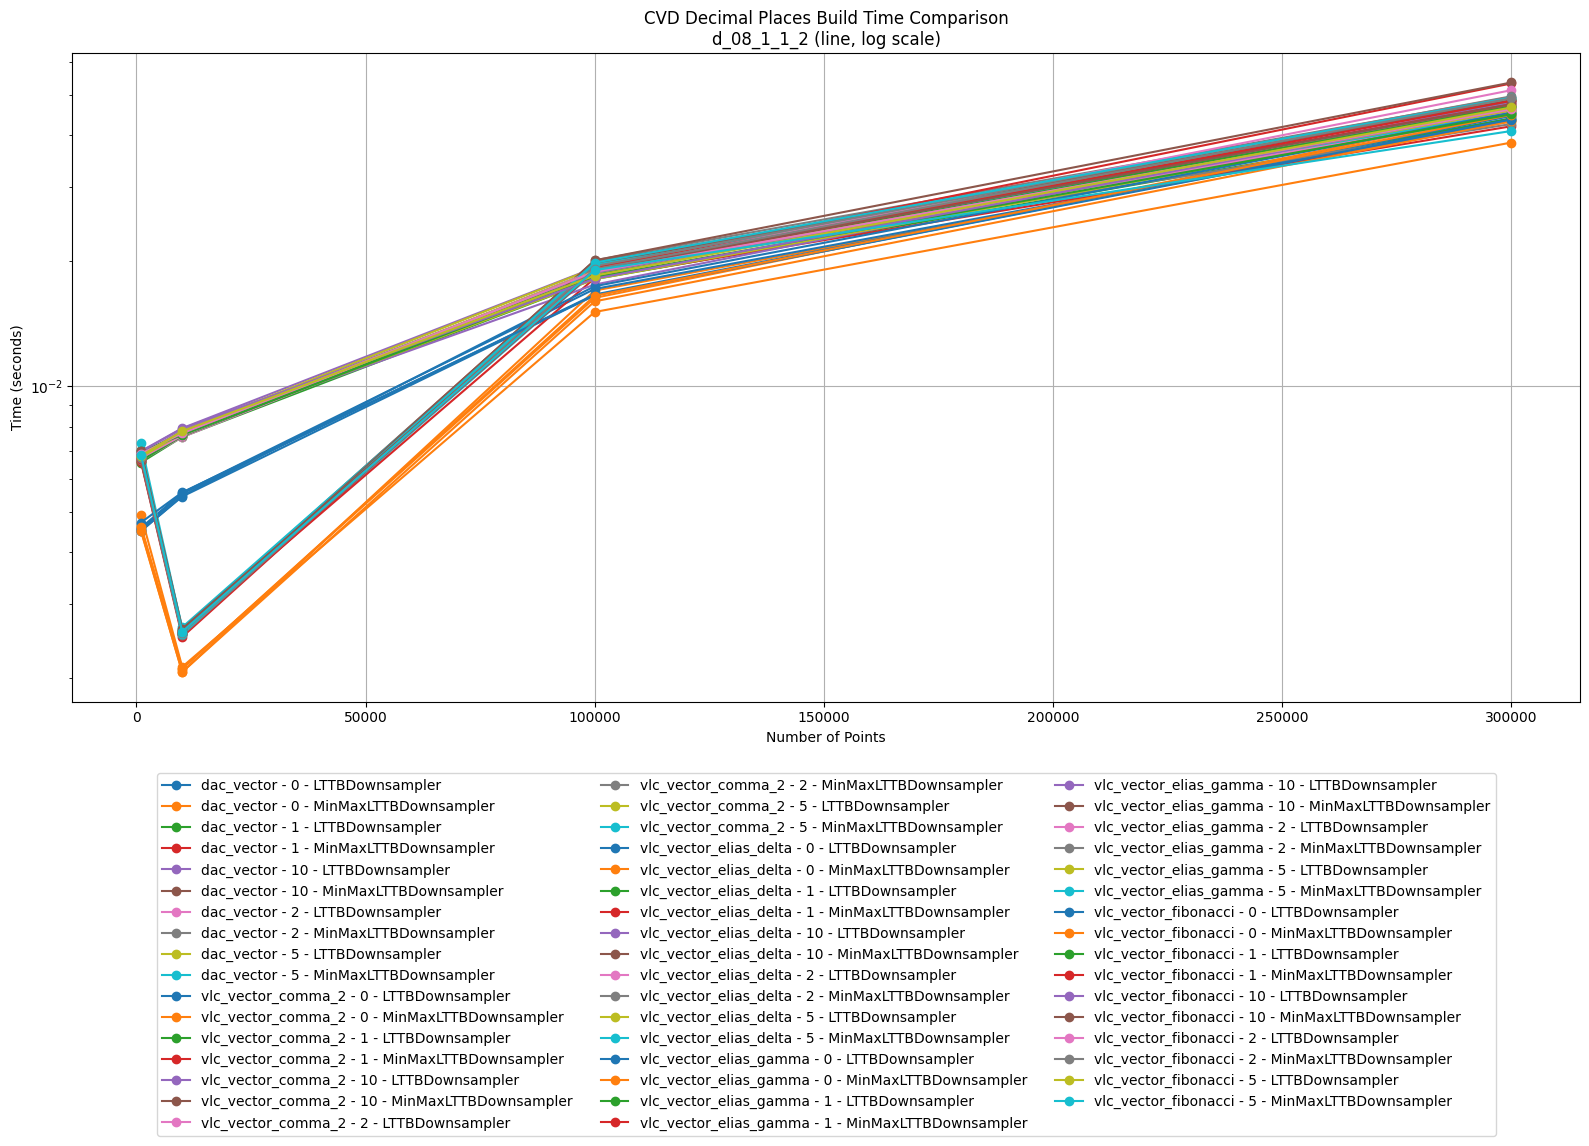
\includegraphics[width=1\textwidth]{anexo/exp/CVD Decimal Places Build Time Comparison/plots/CVD Decimal Places Build Time Comparison_d_08_1_1_2_log_line.png}
        \caption[]{Gráfico de tiempo de construcción CVD con diferentes lugares decimales para el input \textbf{d\_08\_1\_1\_2} en escala logarítmica.}
        \label{fig:cvd_decimal_places_build_time_comparison_plot_log_1}
    \end{figure}
}

\DeclareRobustCommand{\CVDDecimalPlacesBuildTimeComparisonTwoPlotLine}{
    \begin{figure}[H]
        \centering
        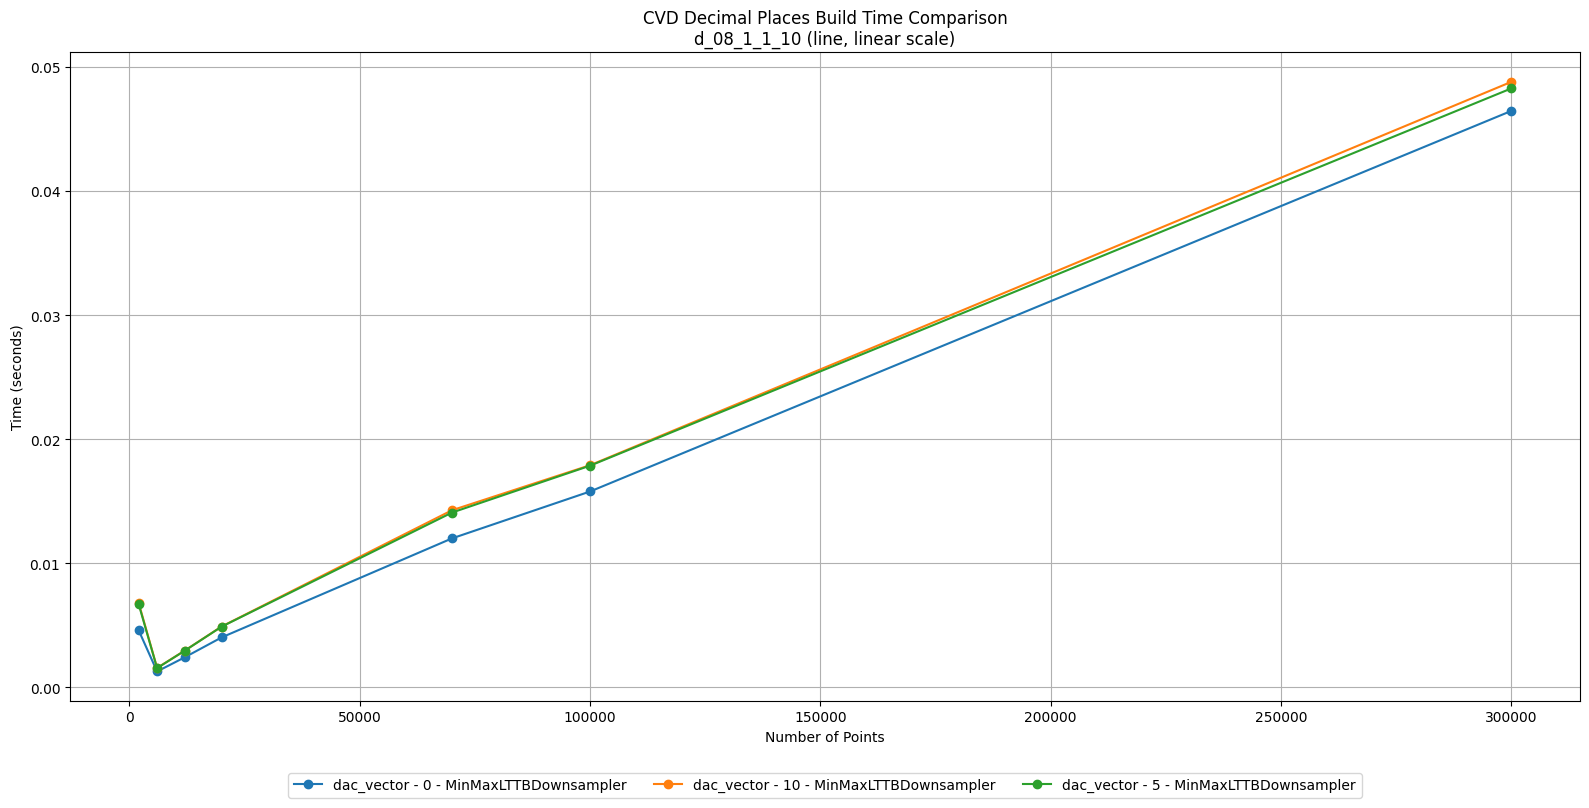
\includegraphics[width=1\textwidth]{anexo/exp/CVD Decimal Places Build Time Comparison/plots/CVD Decimal Places Build Time Comparison_d_08_1_1_10_linear_line.png}
        \caption[]{Gráfico de tiempo de construcción CVD con diferentes lugares decimales para el input \textbf{d\_08\_1\_1\_10}.}
        \label{fig:cvd_decimal_places_build_time_comparison_plot_line_2}
    \end{figure}
    \begin{figure}[H]
        \centering
        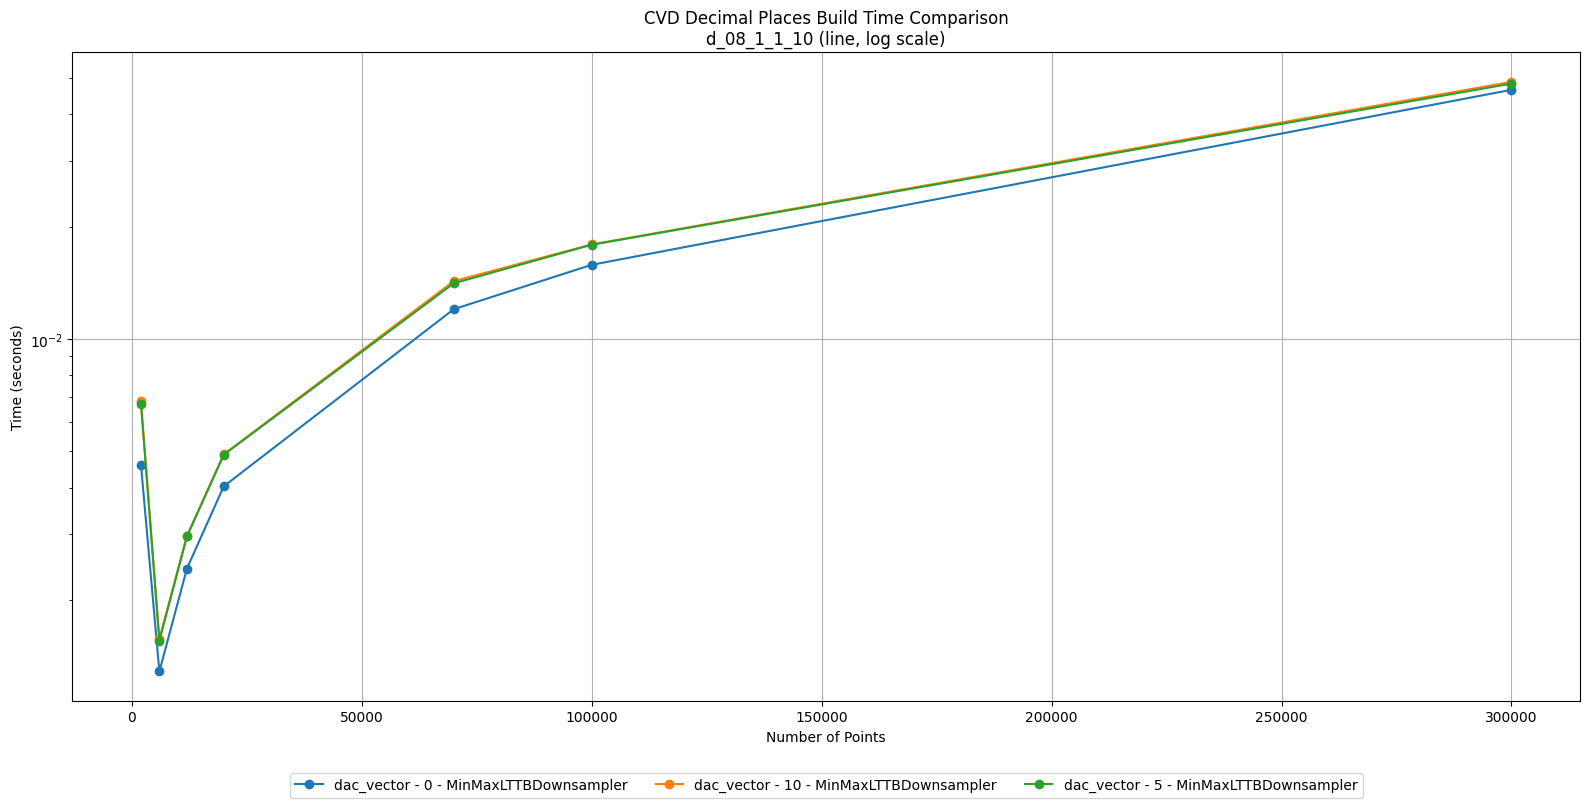
\includegraphics[width=1\textwidth]{anexo/exp/CVD Decimal Places Build Time Comparison/plots/CVD Decimal Places Build Time Comparison_d_08_1_1_10_log_line.png}
        \caption[]{Gráfico de tiempo de construcción CVD con diferentes lugares decimales para el input \textbf{d\_08\_1\_1\_10} en escala logarítmica.}
        \label{fig:cvd_decimal_places_build_time_comparison_plot_log_2}
    \end{figure}
}

\DeclareRobustCommand{\CVDDecimalPlacesBuildTimeComparisonThreePlotLine}{
    \begin{figure}[H]
        \centering
        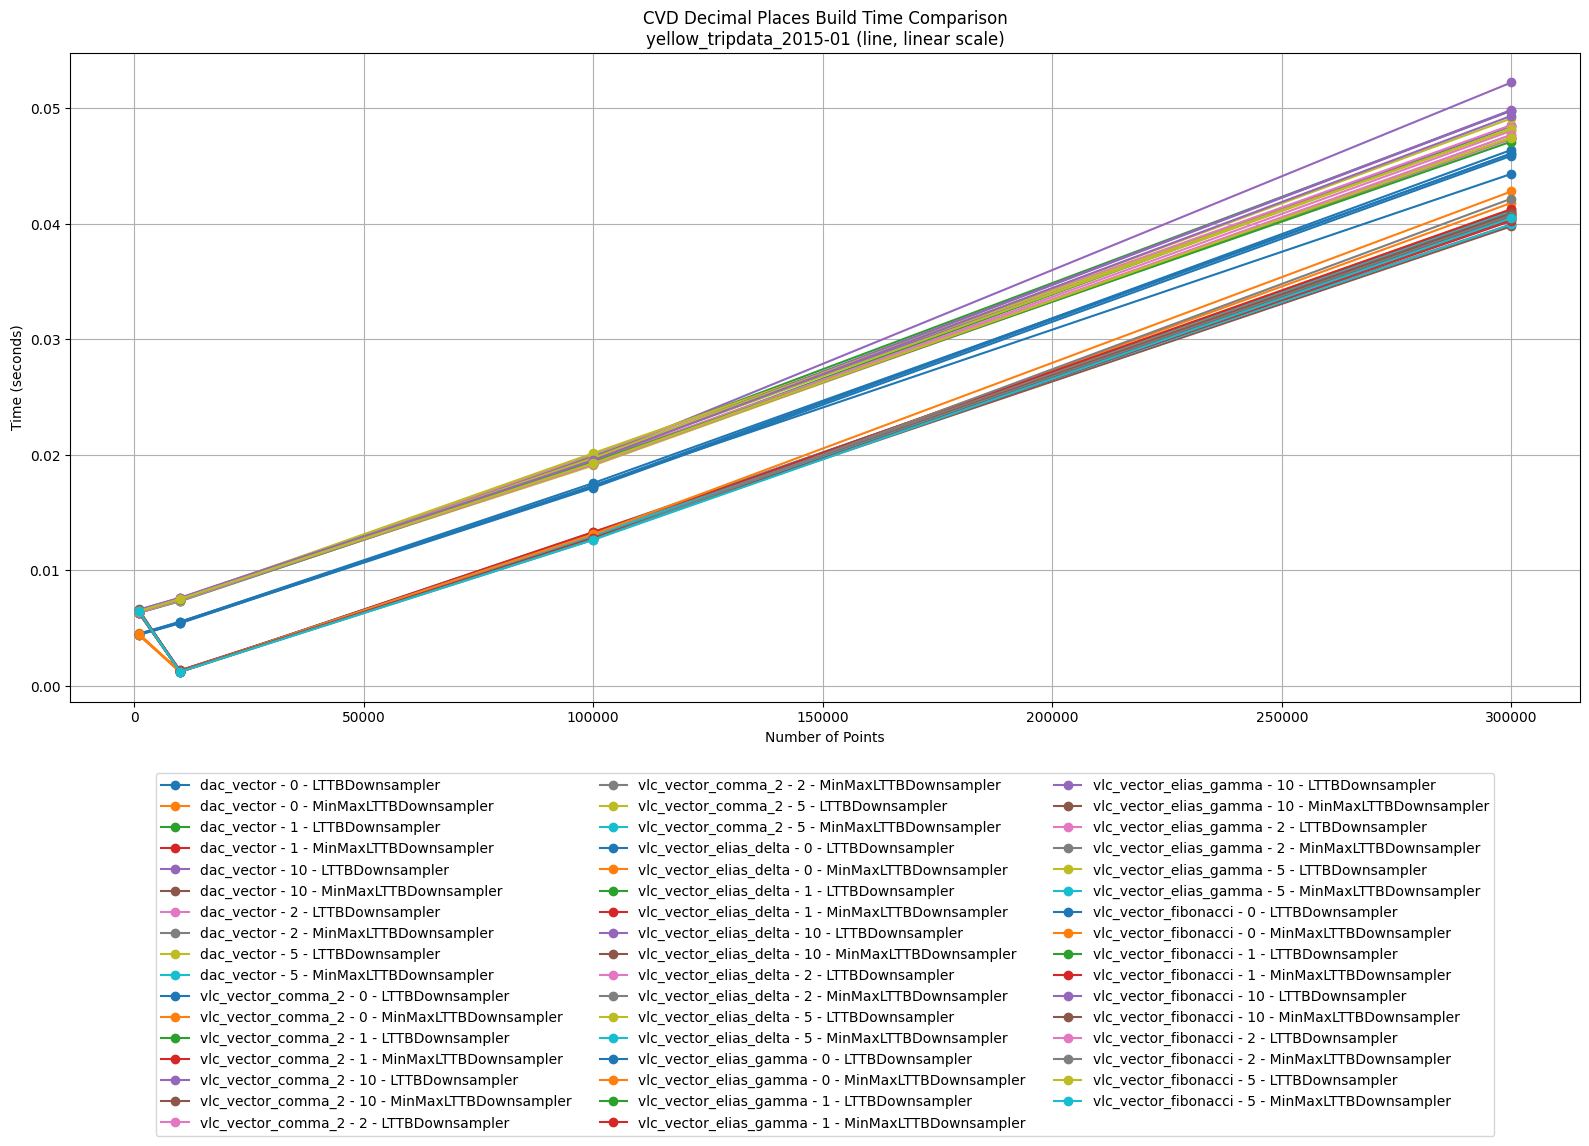
\includegraphics[width=1\textwidth]{anexo/exp/CVD Decimal Places Build Time Comparison/plots/CVD Decimal Places Build Time Comparison_yellow_tripdata_2015-01_linear_line.png}
        \caption[]{Gráfico de tiempo de construcción CVD con diferentes lugares decimales para el input \textbf{yellow\_tripdata\_2015\_01}.}
        \label{fig:cvd_decimal_places_build_time_comparison_plot_line_3}
    \end{figure}
    \begin{figure}[H]
        \centering
        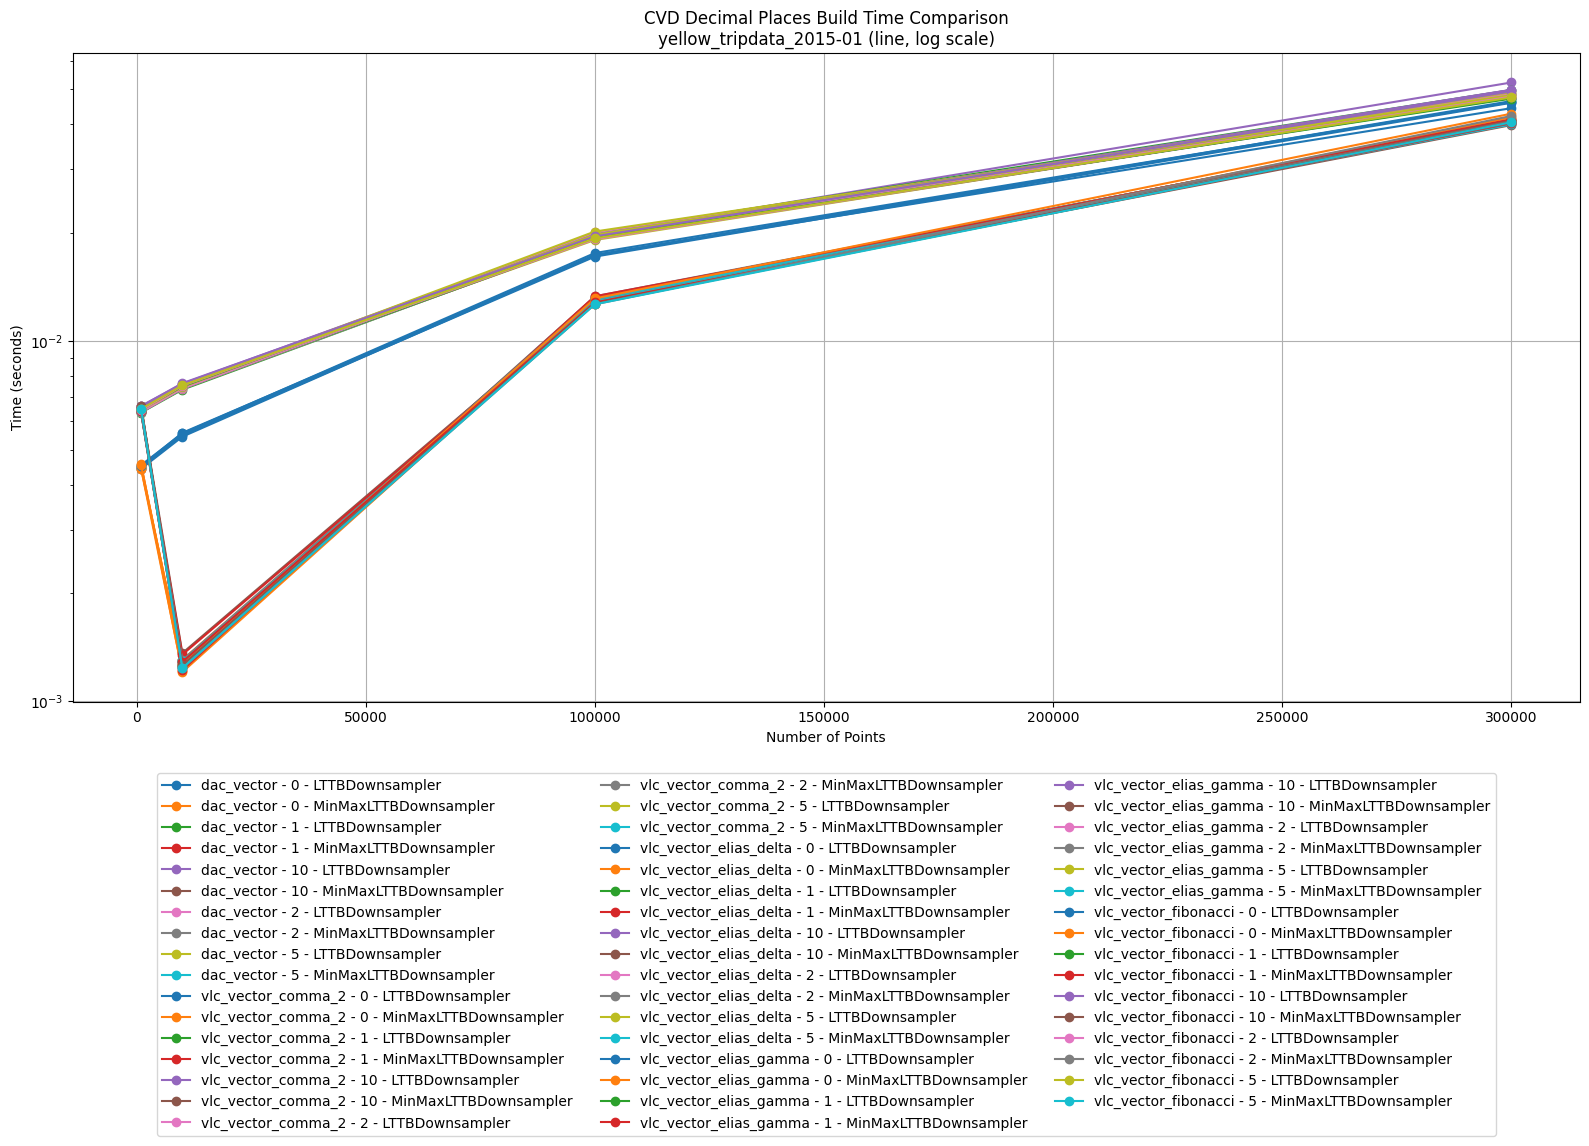
\includegraphics[width=1\textwidth]{anexo/exp/CVD Decimal Places Build Time Comparison/plots/CVD Decimal Places Build Time Comparison_yellow_tripdata_2015-01_log_line.png}
        \caption[]{Gráfico de tiempo de construcción CVD con diferentes lugares decimales para el input \textbf{yellow\_tripdata\_2015\_01} en escala logarítmica.}
        \label{fig:cvd_decimal_places_build_time_comparison_plot_log_3}
    \end{figure}
}


% ===========================
% CVD Decimal Places Size Comparison
% ===========================
\DeclareRobustCommand{\CVDDecimalPlacesSizeComparisonOnePlotLine}{
    \begin{figure}[H]
        \centering
        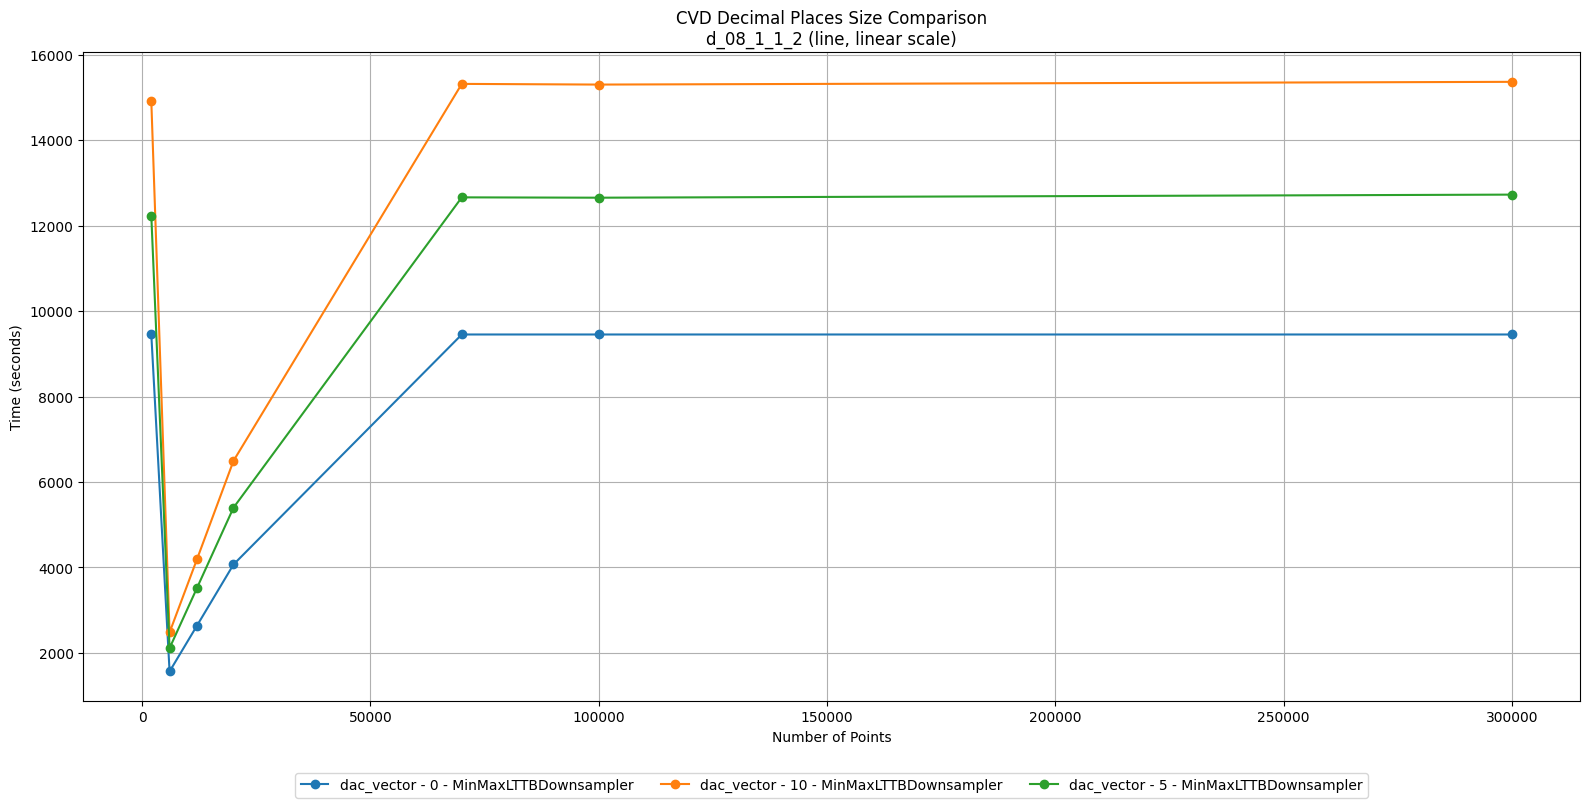
\includegraphics[width=1\textwidth]{anexo/exp/CVD Decimal Places Size Comparison/plots/CVD Decimal Places Size Comparison_d_08_1_1_2_linear_line.png}
        \caption[]{Gráfico de tamaño CVD con diferentes lugares decimales para el input \textbf{d\_08\_1\_1\_2}.}
        \label{fig:cvd_decimal_places_size_comparison_plot_line_1}
    \end{figure}
    \begin{figure}[H]
        \centering
        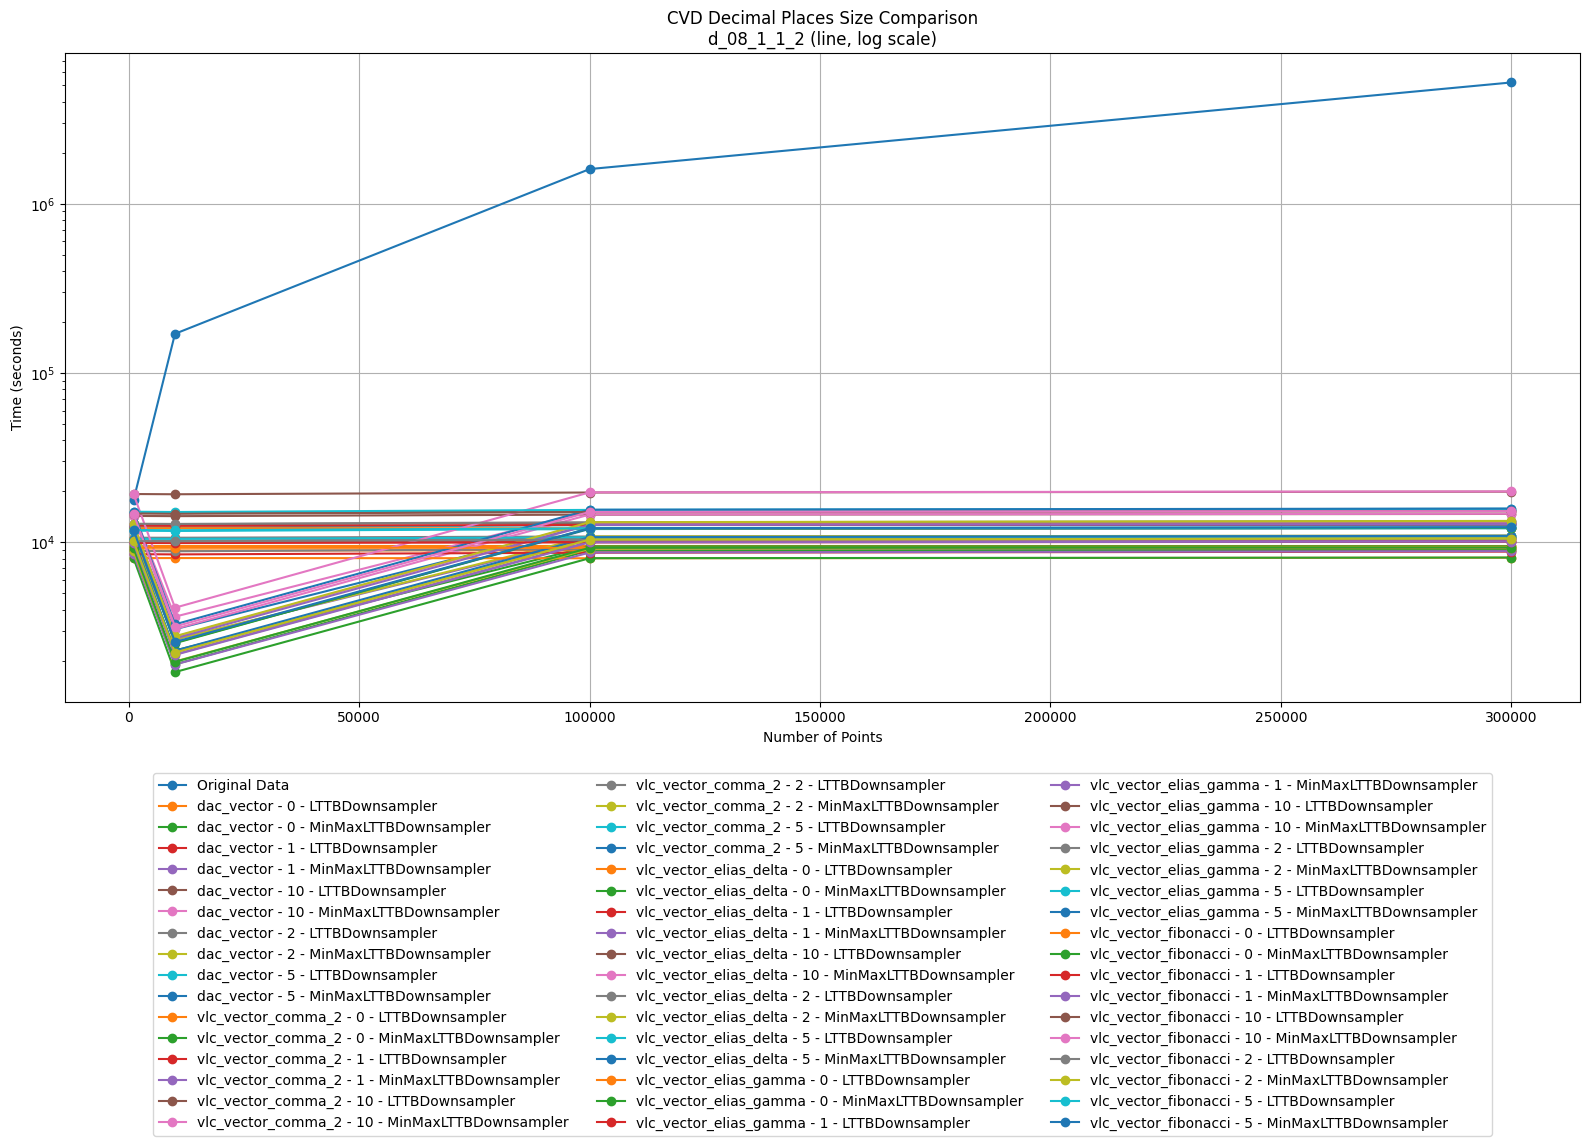
\includegraphics[width=1\textwidth]{anexo/exp/CVD Decimal Places Size Comparison/plots/CVD Decimal Places Size Comparison_d_08_1_1_2_log_line.png}
        \caption[]{Gráfico de tamaño CVD con diferentes lugares decimales para el input \textbf{d\_08\_1\_1\_2} en escala logarítmica.}
        \label{fig:cvd_decimal_places_size_comparison_plot_log_1}
    \end{figure}
}

\DeclareRobustCommand{\CVDDecimalPlacesSizeComparisonTwoPlotLine}{
    \begin{figure}[H]
        \centering
        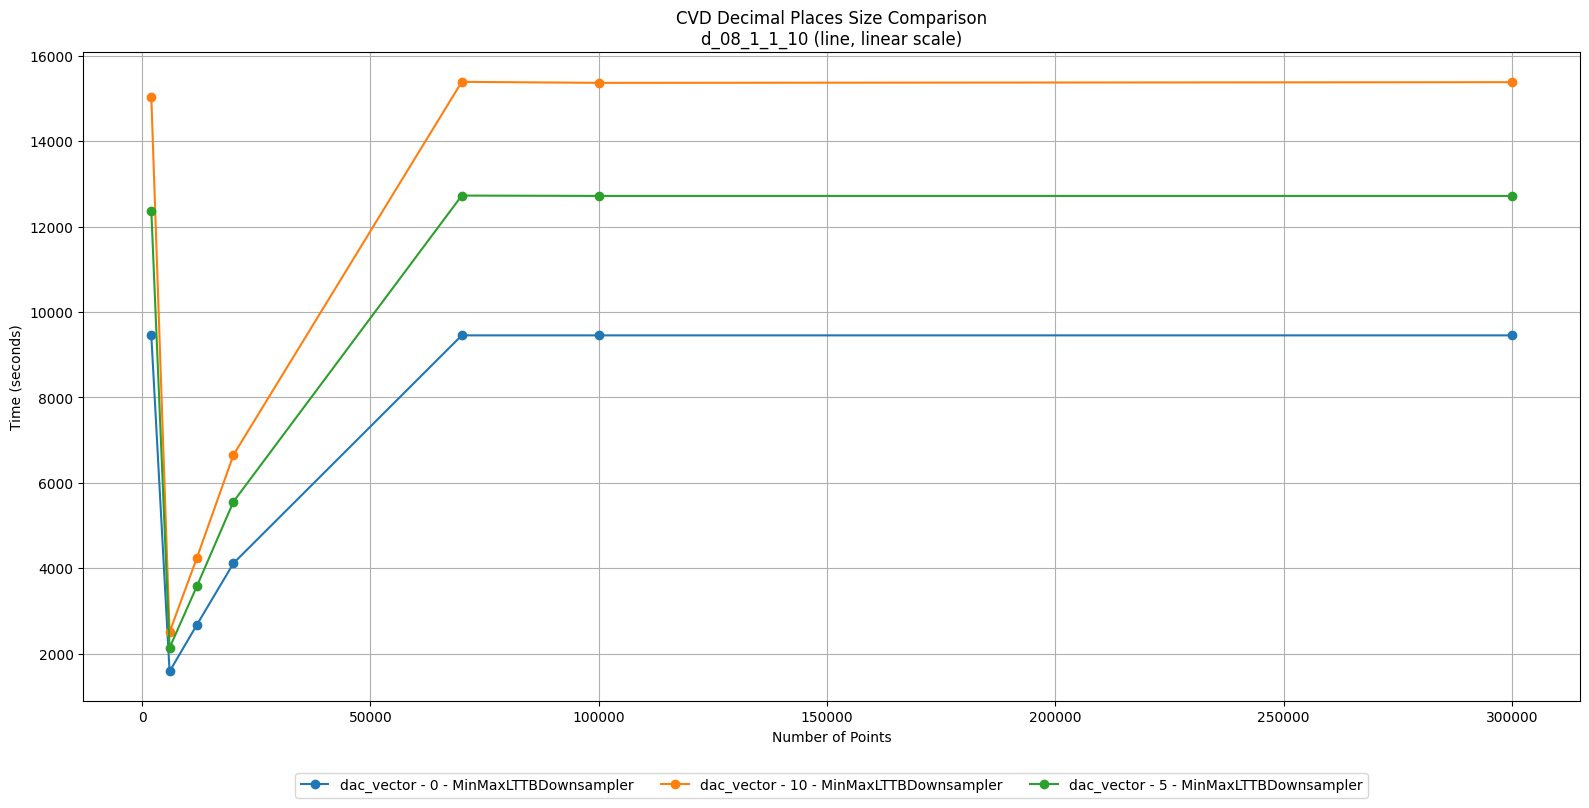
\includegraphics[width=1\textwidth]{anexo/exp/CVD Decimal Places Size Comparison/plots/CVD Decimal Places Size Comparison_d_08_1_1_10_linear_line.png}
        \caption[]{Gráfico de tamaño CVD con diferentes lugares decimales para el input \textbf{d\_08\_1\_1\_10}.}
        \label{fig:cvd_decimal_places_size_comparison_plot_line_2}
    \end{figure}
    \begin{figure}[H]
        \centering
        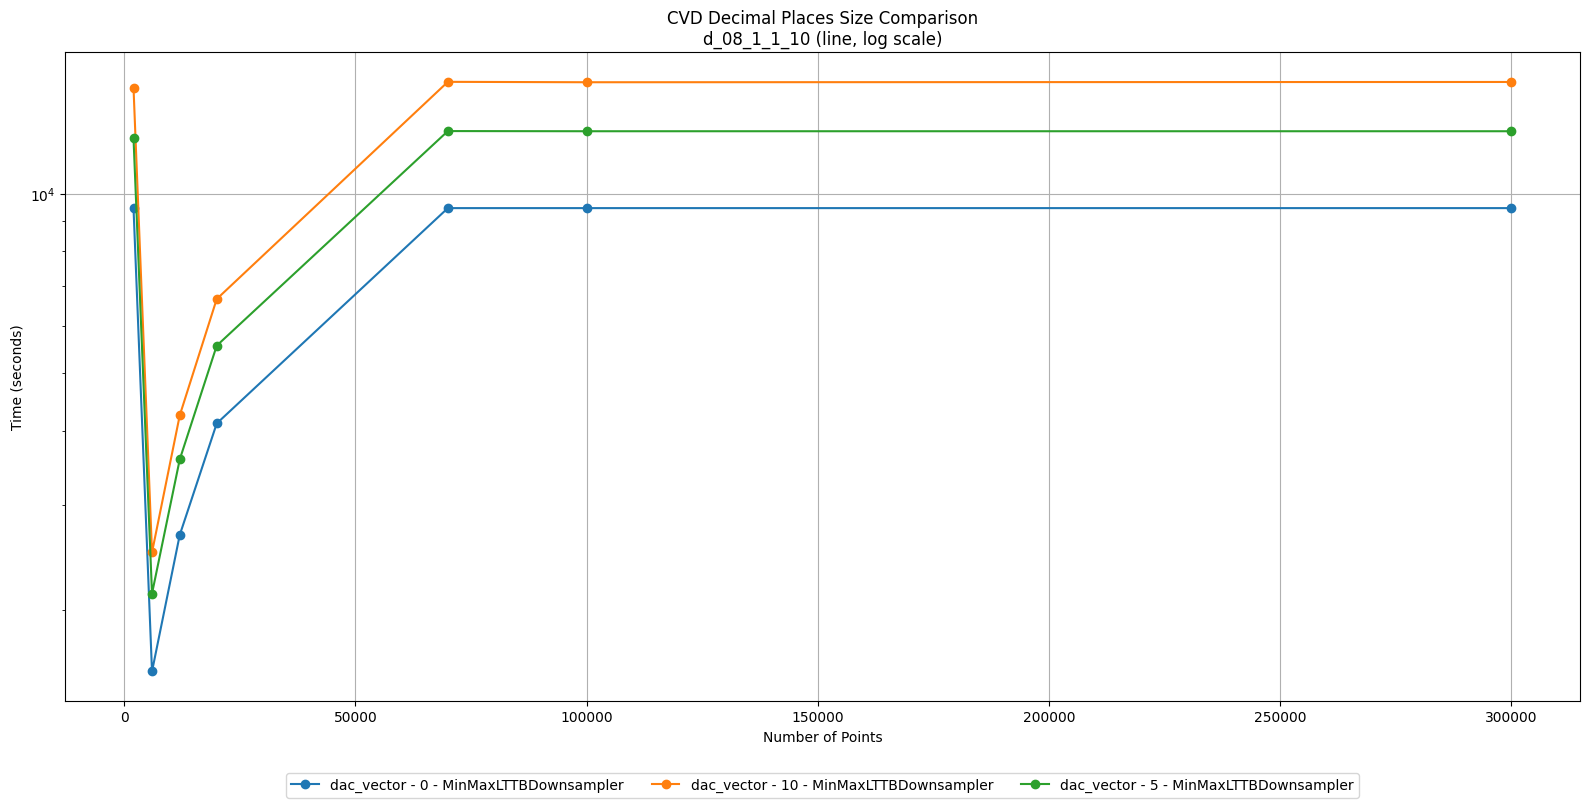
\includegraphics[width=1\textwidth]{anexo/exp/CVD Decimal Places Size Comparison/plots/CVD Decimal Places Size Comparison_d_08_1_1_10_log_line.png}
        \caption[]{Gráfico de tamaño CVD con diferentes lugares decimales para el input \textbf{d\_08\_1\_1\_10} en escala logarítmica.}
        \label{fig:cvd_decimal_places_size_comparison_plot_log_2}
    \end{figure}
}

\DeclareRobustCommand{\CVDDecimalPlacesSizeComparisonThreePlotLine}{
    \begin{figure}[H]
        \centering
        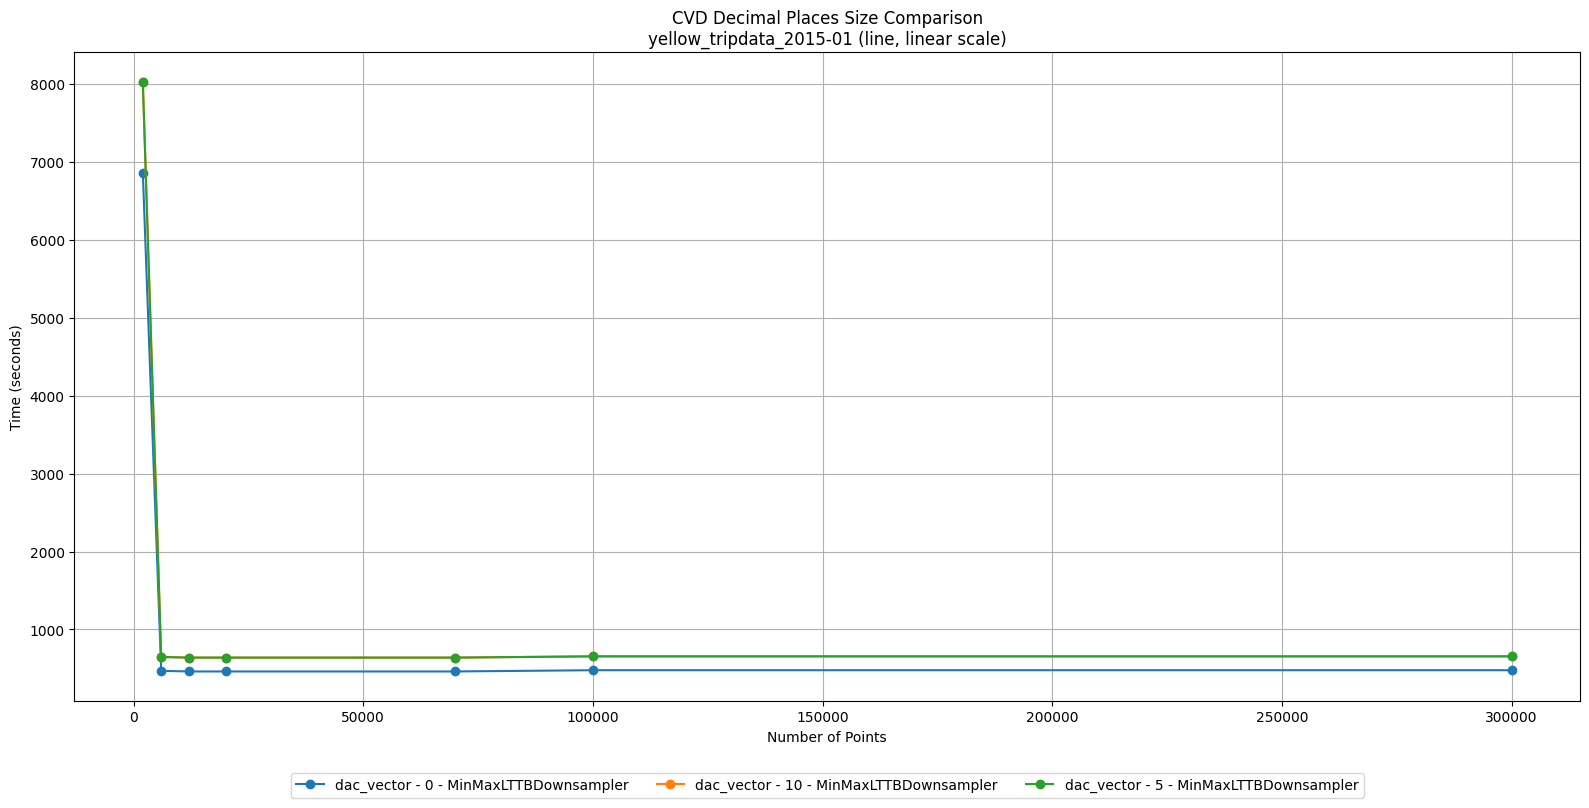
\includegraphics[width=1\textwidth]{anexo/exp/CVD Decimal Places Size Comparison/plots/CVD Decimal Places Size Comparison_yellow_tripdata_2015-01_linear_line.png}
        \caption[]{Gráfico de tamaño CVD con diferentes lugares decimales para el input \textbf{yellow\_tripdata\_2015\_01}.}
        \label{fig:cvd_decimal_places_size_comparison_plot_line_3}
    \end{figure}
    \begin{figure}[H]
        \centering
        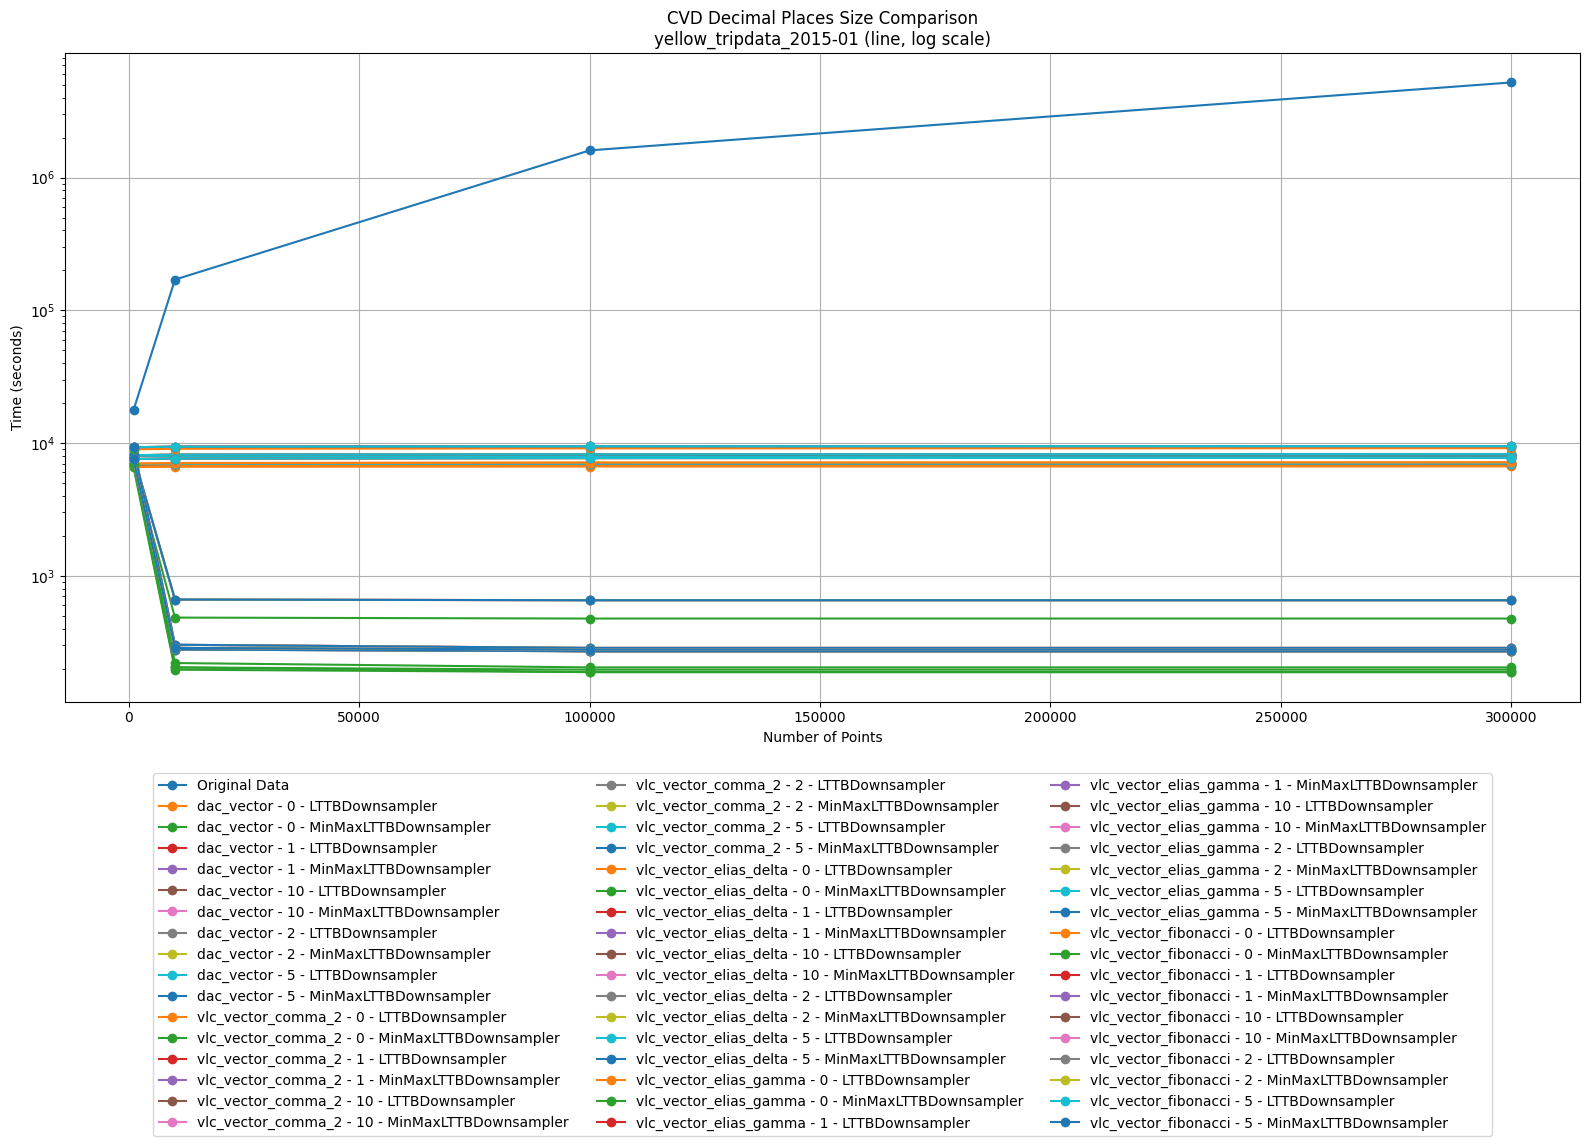
\includegraphics[width=1\textwidth]{anexo/exp/CVD Decimal Places Size Comparison/plots/CVD Decimal Places Size Comparison_yellow_tripdata_2015-01_log_line.png}
        \caption[]{Gráfico de tamaño CVD con diferentes lugares decimales para el input \textbf{yellow\_tripdata\_2015\_01} en escala logarítmica.}
        \label{fig:cvd_decimal_places_size_comparison_plot_log_3}
    \end{figure}
}





% PyGal Plotting Memory Allocation
\DeclareRobustCommand{\PyGalMemoryAllocationOnePlotLine}{
    %insertar imagen
    \begin{figure}[H]
        \centering
        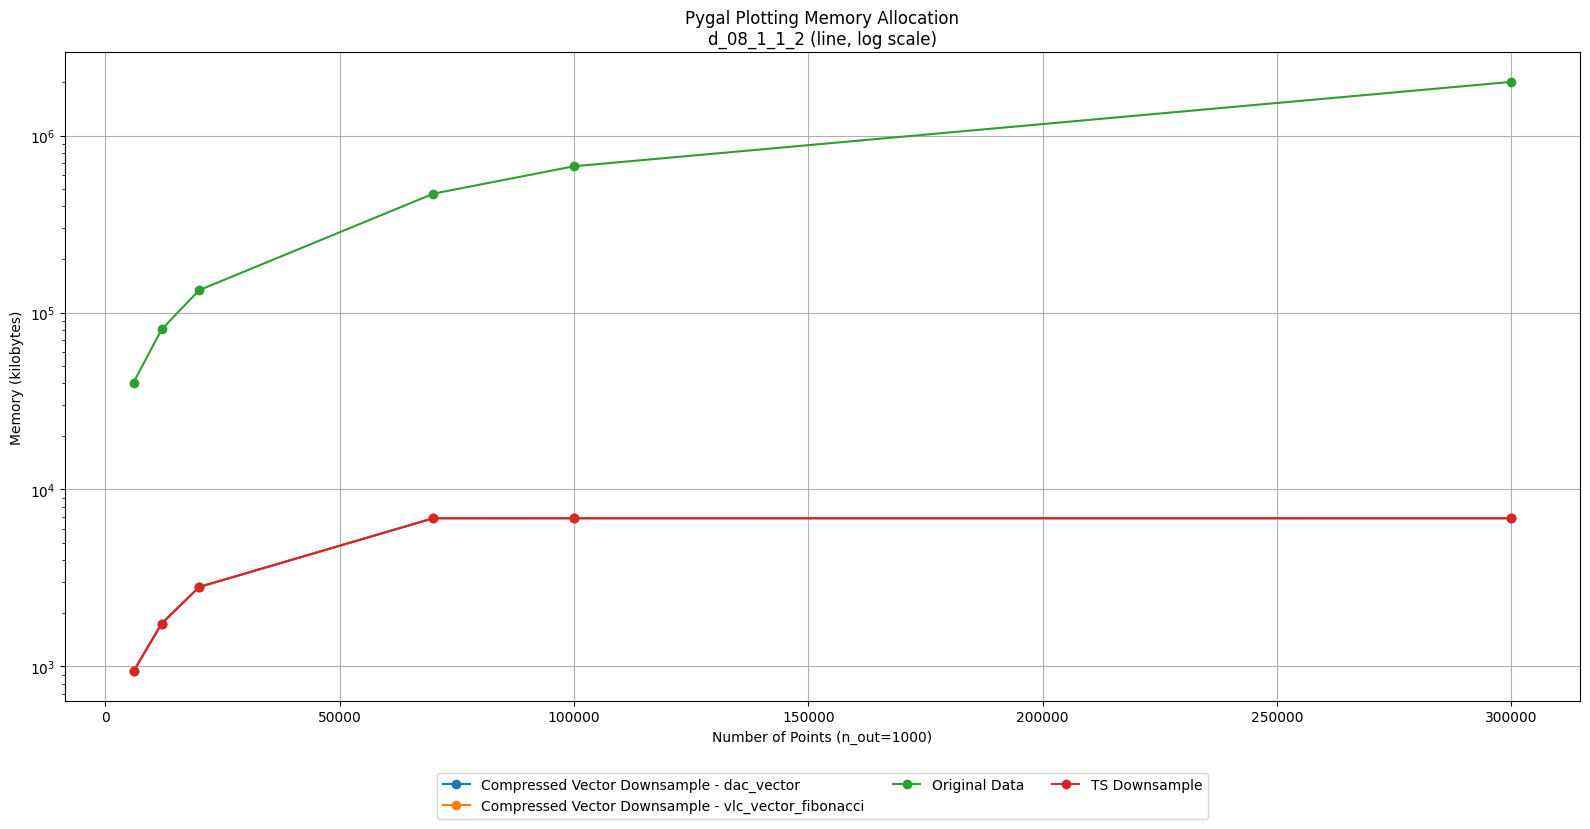
\includegraphics[width=1\textwidth]{anexo/exp/Pygal Plotting Memory Allocation/plots/Pygal Plotting Memory Allocation_d_08_1_1_2_log_line.png}
        \caption[]{Gráfico de memoria asignada por PyGal para el input \textbf{d\_08\_1\_1\_2}.}
        \label{fig:pygal_memory_allocation_plot_line_1}
    \end{figure}
}

\DeclareRobustCommand{\PyGalMemoryAllocationOnePlotBar}{
    %insertar imagen
    \begin{figure}[H]
        \centering
        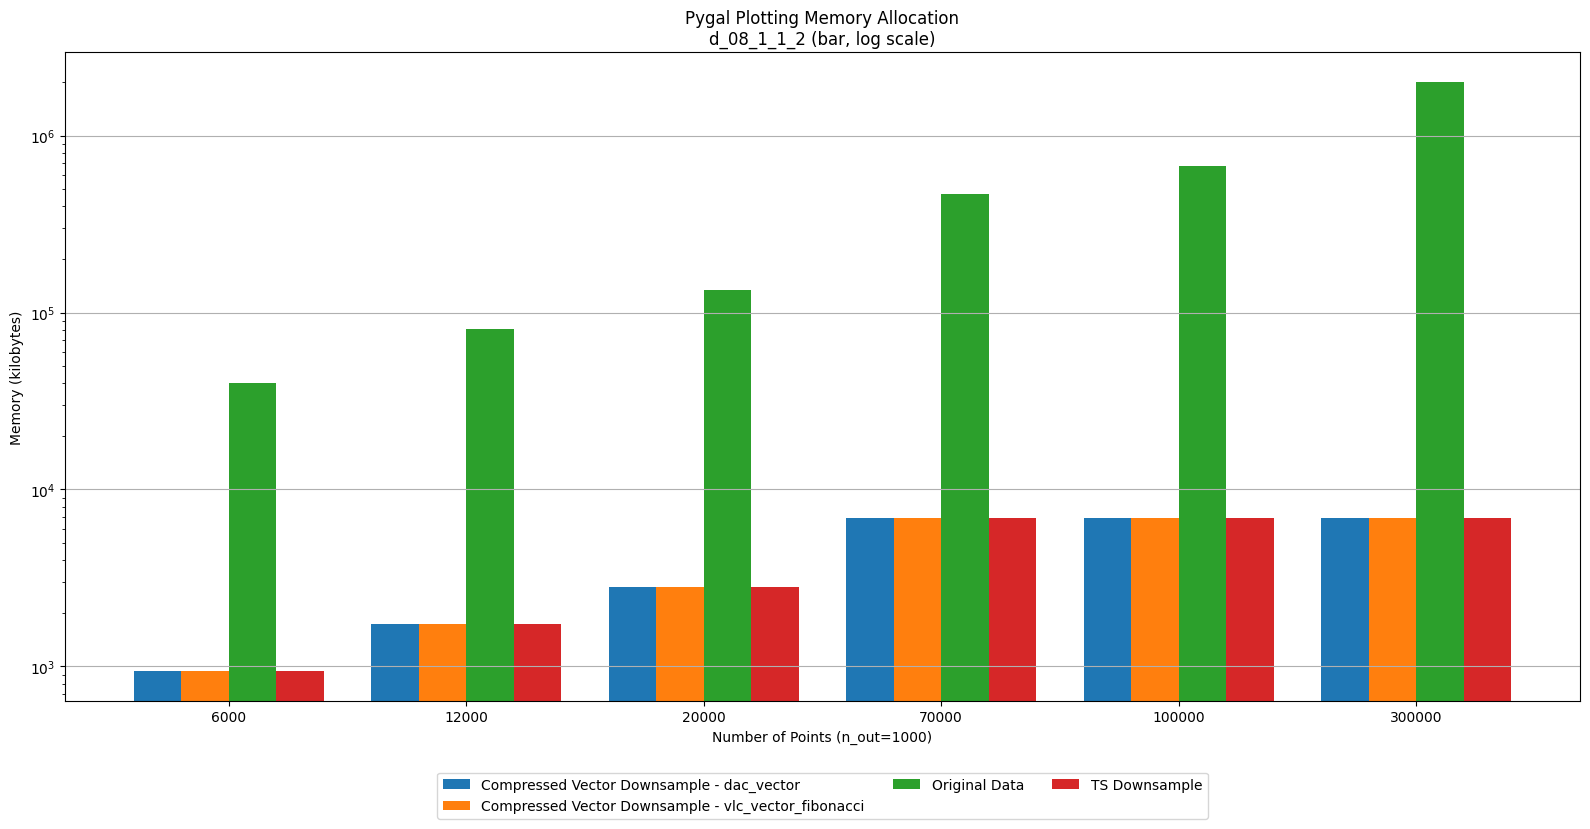
\includegraphics[width=1\textwidth]{anexo/exp/Pygal Plotting Memory Allocation/bar_plots/Pygal Plotting Memory Allocation_d_08_1_1_2_log_bar.png}
        \caption[]{Gráfico de memoria asignada por PyGal para el input \textbf{d\_08\_1\_1\_2}.}
        \label{fig:pygal_memory_allocation_plot_bar_1}
    \end{figure}
\begin{table}[H]
\centering
\resizebox{\textwidth}{!}{%
\begin{tabular}{|l|c|c|c|c|c|c|}
\hline\multicolumn{1}{|c|}{Option} & \multicolumn{6}{c|}{\textbf{Number of data points}} \\
\cline{2-7}
 & \textbf{6000} & \textbf{12000} & \textbf{20000} & \textbf{70000} & \textbf{100000} & \textbf{300000} \\
\hline
Compressed Vector Downsample - dac\_vector & 9.38e+02 [kb] & 1.75e+03 [kb] & 2.81e+03 [kb] & 6.88e+03 [kb] & 6.88e+03 [kb] & 6.88e+03 [kb] \\
Compressed Vector Downsample - vlc\_vector\_fibonacci & 9.38e+02 [kb] & 1.75e+03 [kb] & 2.81e+03 [kb] & 6.88e+03 [kb] & 6.88e+03 [kb] & 6.88e+03 [kb] \\
Original Data & 4.02e+04 [kb] & 8.03e+04 [kb] & 1.34e+05 [kb] & 4.70e+05 [kb] & 6.71e+05 [kb] & 2.01e+06 [kb] \\
TS Downsample & 9.37e+02 [kb] & 1.75e+03 [kb] & 2.81e+03 [kb] & 6.88e+03 [kb] & 6.88e+03 [kb] & 6.88e+03 [kb] \\
\hline
\end{tabular}
}
\label{tab:pygal plotting memory allocation-d-08-1-1-2}
\end{table}
   \begin{table}[H]
\centering
\caption{\textit{d\_08\_1\_1\_2} – Memoria por elemento}
\label{tab:d\_08\_1\_1\_2_mem_por_elemento_sin_original}
\begin{tabular}{rrrr}
\toprule
 & CVD - dac\_vector & CVD - vlc\_vector\_fibonacci & TS Downsample \\
n\_size &  &  &  \\
\midrule
6000 & 0.94 & 0.94 & 0.94 \\
12000 & 1.75 & 1.75 & 1.75 \\
20000 & 2.81 & 2.81 & 2.81 \\
70000 & 6.88 & 6.88 & 6.88 \\
100000 & 6.88 & 6.88 & 6.88 \\
300000 & 6.88 & 6.88 & 6.88 \\
\bottomrule
\end{tabular}

\end{table}
}

\DeclareRobustCommand{\PyGalMemoryAllocationTwoPlotLine}{
    %insertar imagen
    \begin{figure}[H]
        \centering
        \includegraphics[width=1\textwidth]{anexo/exp/PyGal Plotting Memory Allocation/plots/PyGal Plotting Memory Allocation_d_08_1_1_10_linear_line.png}
        \caption[]{Gráfico de memoria asignada por PyGal para el input \textbf{d\_08\_1\_1\_10}.}
        \label{fig:pygal_memory_allocation_plot_line_2}
    \end{figure}
}

\DeclareRobustCommand{\PyGalMemoryAllocationTwoPlotBar}{
    %insertar imagen
    \begin{figure}[H]
        \centering
        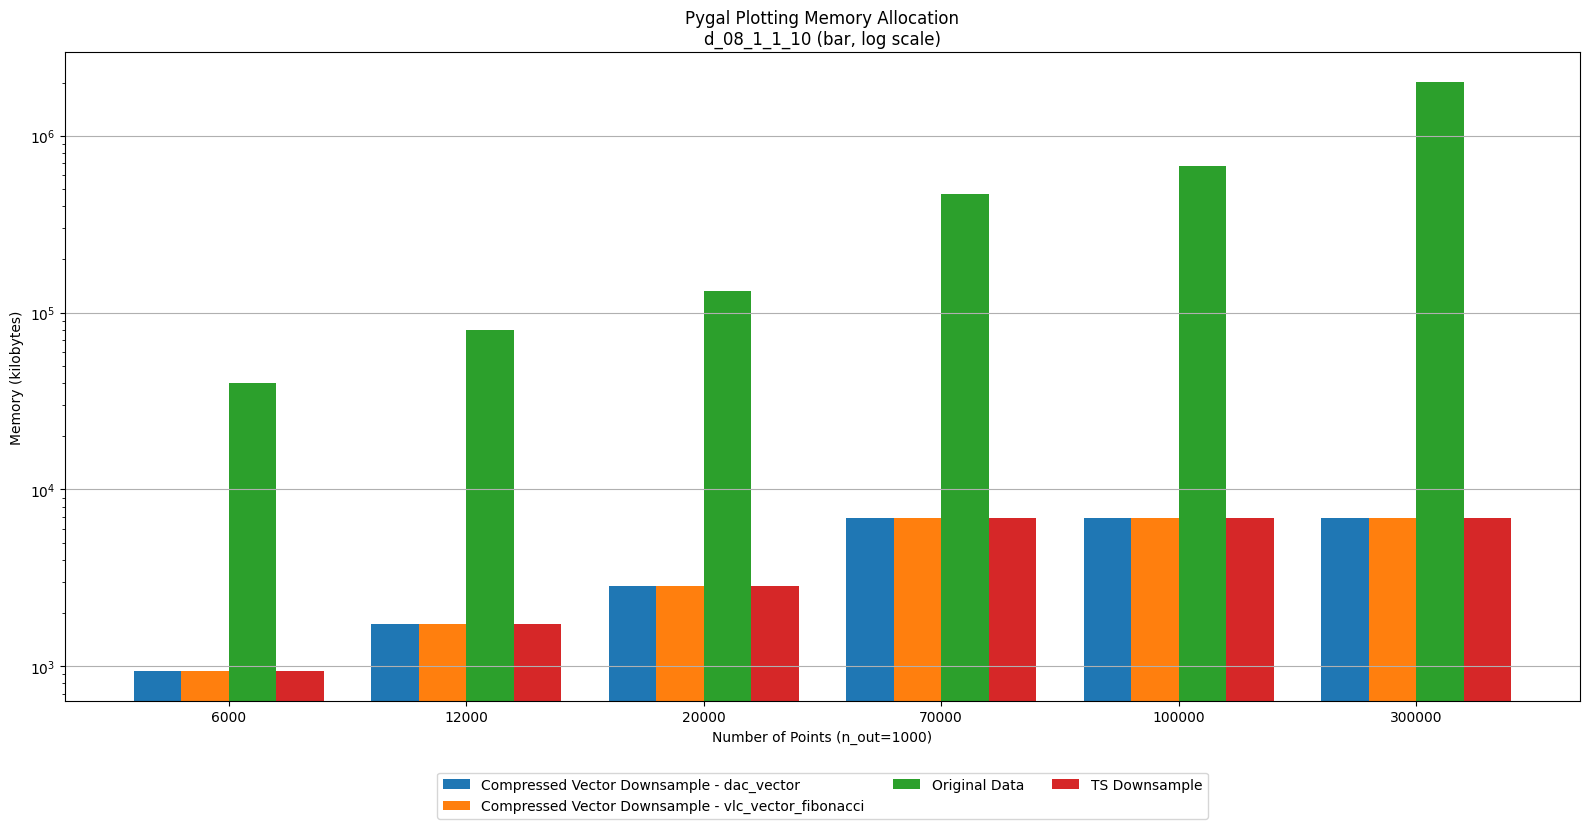
\includegraphics[width=1\textwidth]{anexo/exp/Pygal Plotting Memory Allocation/bar_plots/Pygal Plotting Memory Allocation_d_08_1_1_10_log_bar.png}
        \caption[]{Gráfico de memoria asignada por PyGal para el input \textbf{d\_08\_1\_1\_10}.}
        \label{fig:pygal_memory_allocation_plot_bar_2}
    \end{figure}

\begin{table}[H]
\centering
\resizebox{\textwidth}{!}{%
\begin{tabular}{|l|c|c|c|c|c|c|}
\hline\multicolumn{1}{|c|}{Option} & \multicolumn{6}{c|}{\textbf{Number of data points}} \\
\cline{2-7}
 & \textbf{6000} & \textbf{12000} & \textbf{20000} & \textbf{70000} & \textbf{100000} & \textbf{300000} \\
\hline
Compressed Vector Downsample - dac_vector & 9.36e+02 [kb] & 1.74e+03 [kb] & 2.83e+03 [kb] & 6.88e+03 [kb] & 6.88e+03 [kb] & 6.89e+03 [kb] \\
Compressed Vector Downsample - vlc_vector_fibonacci & 9.36e+02 [kb] & 1.75e+03 [kb] & 2.83e+03 [kb] & 6.88e+03 [kb] & 6.88e+03 [kb] & 6.89e+03 [kb] \\
Original Data & 4.01e+04 [kb] & 8.01e+04 [kb] & 1.33e+05 [kb] & 4.70e+05 [kb] & 6.71e+05 [kb] & 2.02e+06 [kb] \\
TS Downsample & 9.36e+02 [kb] & 1.74e+03 [kb] & 2.83e+03 [kb] & 6.88e+03 [kb] & 6.88e+03 [kb] & 6.90e+03 [kb] \\
\hline
\end{tabular}
}
\label{tab:pygal plotting memory allocation-d-08-1-1-10}
\end{table}
\begin{table}[H]
\centering
\caption{\textit{d\_08\_1\_1\_10} – Memoria por elemento}
\label{tab:d\_08\_1\_1\_10_mem_por_elemento_sin_original}
\begin{tabular}{rrrr}
\toprule
 & CVD - dac\_vector & CVD - vlc\_vector\_fibonacci & TS Downsample \\
n\_size &  &  &  \\
\midrule
6000 & 0.94 & 0.94 & 0.94 \\
12000 & 1.74 & 1.75 & 1.74 \\
20000 & 2.83 & 2.83 & 2.83 \\
70000 & 6.88 & 6.88 & 6.88 \\
100000 & 6.88 & 6.88 & 6.88 \\
300000 & 6.89 & 6.89 & 6.90 \\
\bottomrule
\end{tabular}

\end{table}
}

\DeclareRobustCommand{\PyGalMemoryAllocationThreePlotLine}{
    %insertar imagen
    \begin{figure}[H]
        \centering
        \includegraphics[width=1\textwidth]{anexo/exp/PyGal Plotting Memory Allocation/plots/PyGal Plotting Memory Allocation_yellow_tripdata_2015-01_linear_line.png}
        \caption[]{Gráfico de memoria asignada por PyGal para el input \textbf{yellow\_tripdata\_2015\_01}.}
        \label{fig:pygal_memory_allocation_plot_line_3}
    \end{figure}
}

\DeclareRobustCommand{\PyGalMemoryAllocationThreePlotBar}{
    %insertar imagen
    \begin{figure}[H]
        \centering
        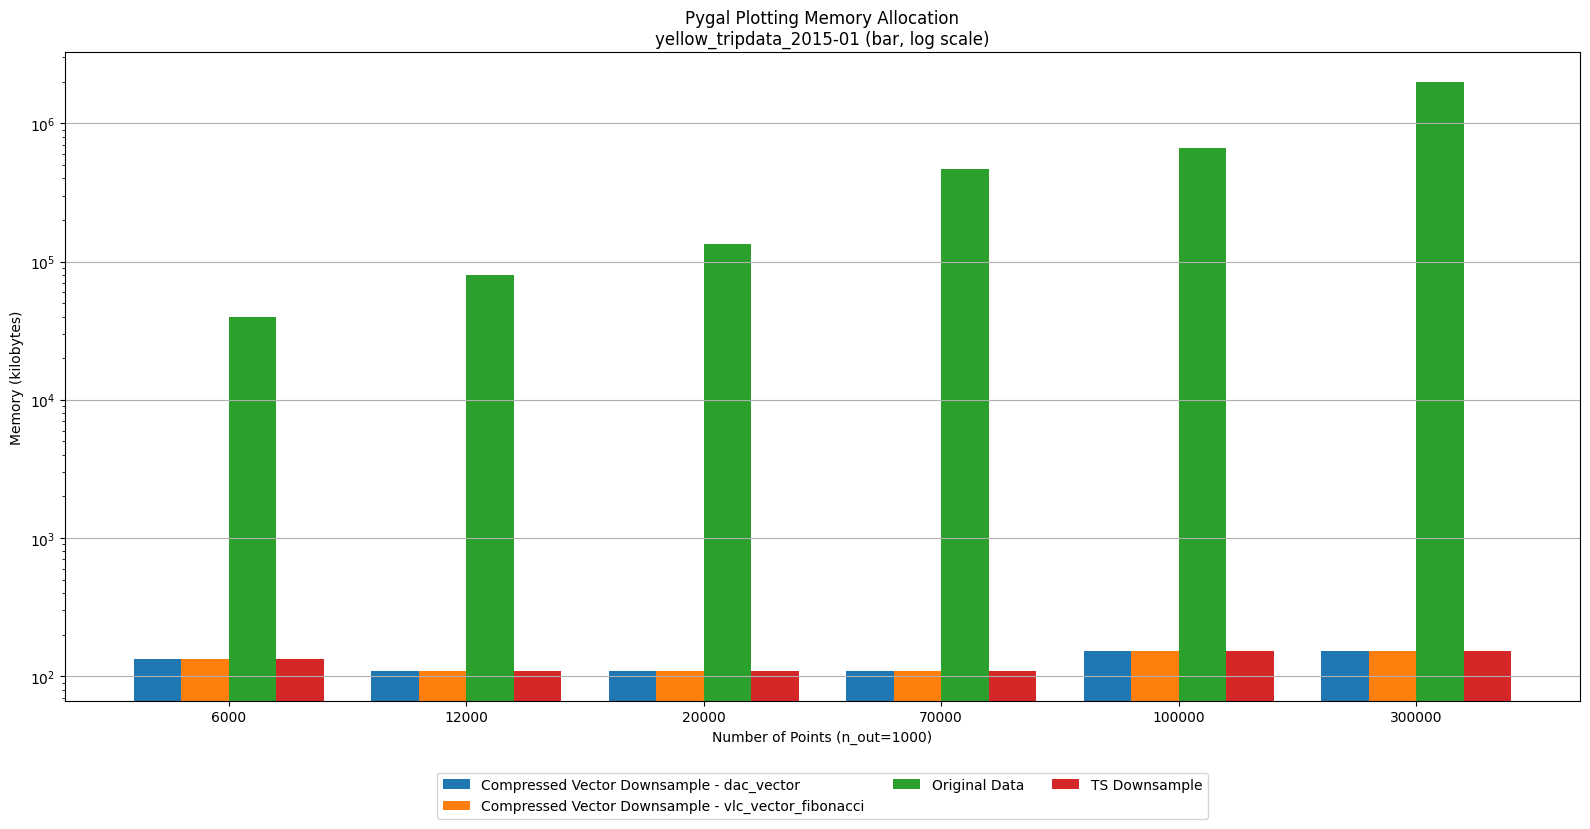
\includegraphics[width=1\textwidth]{anexo/exp/Pygal Plotting Memory Allocation/bar_plots/Pygal Plotting Memory Allocation_yellow_tripdata_2015-01_log_bar.png}
        \caption[]{Gráfico de memoria asignada por PyGal para el input \textbf{yellow\_tripdata\_2015\_01}.}
        \label{fig:pygal_memory_allocation_plot_bar_3}
    \end{figure}
\begin{table}[H]
\centering
\resizebox{\textwidth}{!}{%
\begin{tabular}{|l|c|c|c|c|c|c|}
\hline\multicolumn{1}{|c|}{Option} & \multicolumn{6}{c|}{\textbf{Number of data points}} \\
\cline{2-7}
 & \textbf{6000} & \textbf{12000} & \textbf{20000} & \textbf{70000} & \textbf{100000} & \textbf{300000} \\
\hline
Compressed Vector Downsample - dac_vector & 1.33e+02 [kb] & 1.09e+02 [kb] & 1.09e+02 [kb] & 1.09e+02 [kb] & 1.53e+02 [kb] & 1.52e+02 [kb] \\
Compressed Vector Downsample - vlc_vector_fibonacci & 1.33e+02 [kb] & 1.09e+02 [kb] & 1.10e+02 [kb] & 1.09e+02 [kb] & 1.53e+02 [kb] & 1.53e+02 [kb] \\
Original Data & 4.00e+04 [kb] & 7.99e+04 [kb] & 1.33e+05 [kb] & 4.65e+05 [kb] & 6.64e+05 [kb] & 2.00e+06 [kb] \\
TS Downsample & 1.32e+02 [kb] & 1.09e+02 [kb] & 1.09e+02 [kb] & 1.08e+02 [kb] & 1.53e+02 [kb] & 1.53e+02 [kb] \\
\hline
\end{tabular}
}
\label{tab:pygal plotting memory allocation-yellow-tripdata-2015-01}
\end{table}
\begin{table}[H]
\centering
\caption{\textit{yellow\_tripdata\_2015-01} – Memoria por elemento}
\label{tab:yellow\_tripdata\_2015-01_mem_por_elemento_sin_original}
\begin{tabular}{rrrr}
\toprule
 & CVD - dac\_vector & CVD - vlc\_vector\_fibonacci & TS Downsample \\
n\_size &  &  &  \\
\midrule
6000 & 0.13 & 0.13 & 0.13 \\
12000 & 0.11 & 0.11 & 0.11 \\
20000 & 0.11 & 0.11 & 0.11 \\
70000 & 0.11 & 0.11 & 0.11 \\
100000 & 0.15 & 0.15 & 0.15 \\
300000 & 0.15 & 0.15 & 0.15 \\
\bottomrule
\end{tabular}

\end{table}
}

% PyGal Plot Time
\DeclareRobustCommand{\PyGalPlotTimeOnePlotLine}{
    %insertar imagen
    \begin{figure}[H]
        \centering
        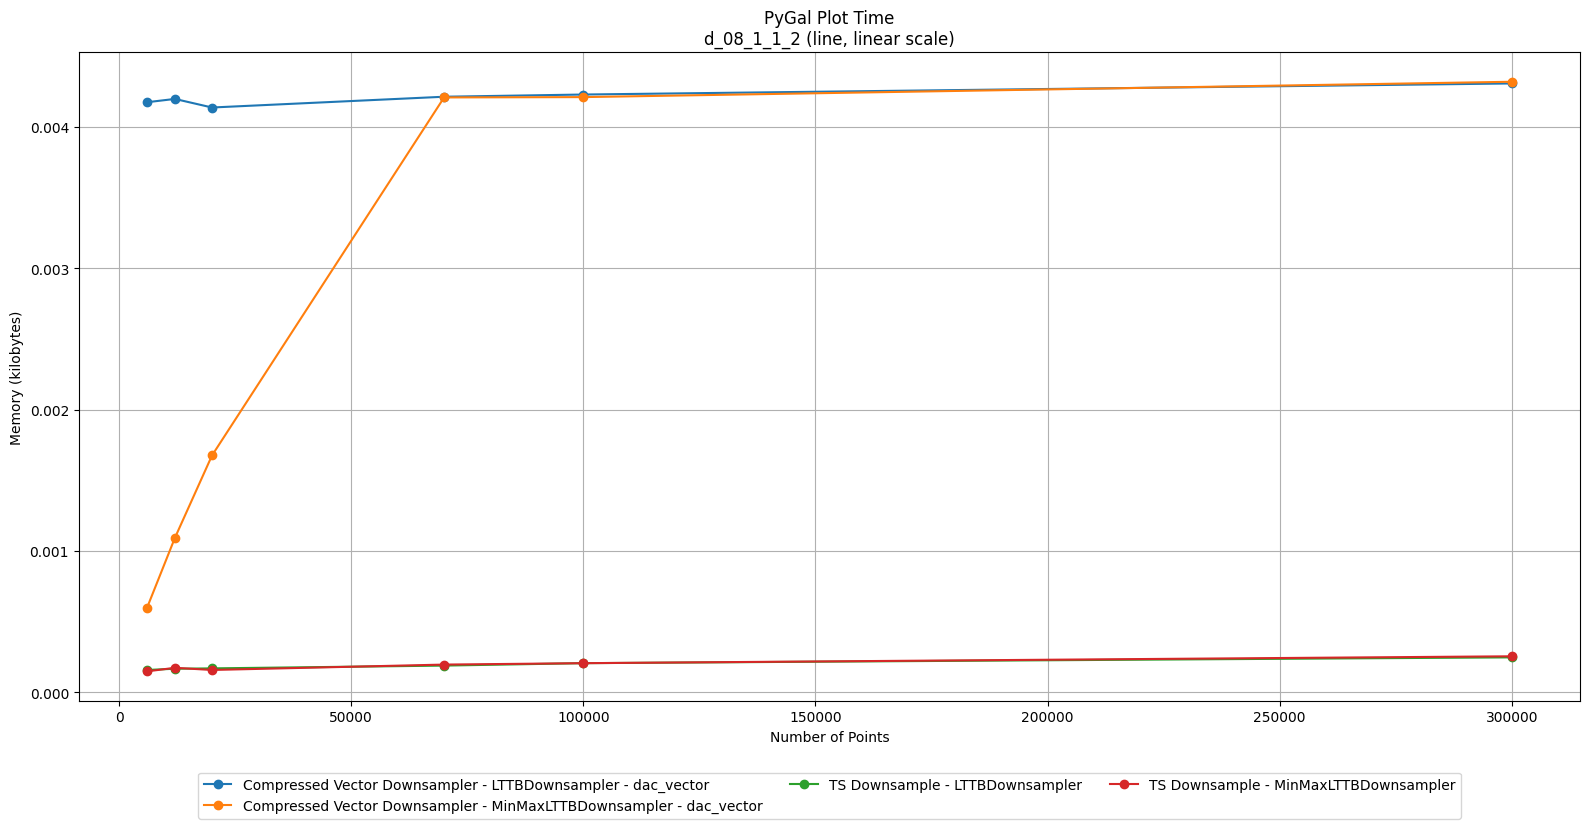
\includegraphics[width=1\textwidth]{anexo/exp/PyGal Plot Time/plots/PyGal Plot Time_d_08_1_1_2_linear_line.png}
        \caption[]{Gráfico de tiempo de renderización PyGal para el input \textbf{d\_08\_1\_1\_2}.}
        \label{fig:pygal_plot_time_plot_line_1}
    \end{figure}
    \begin{figure}[H]
        \centering
        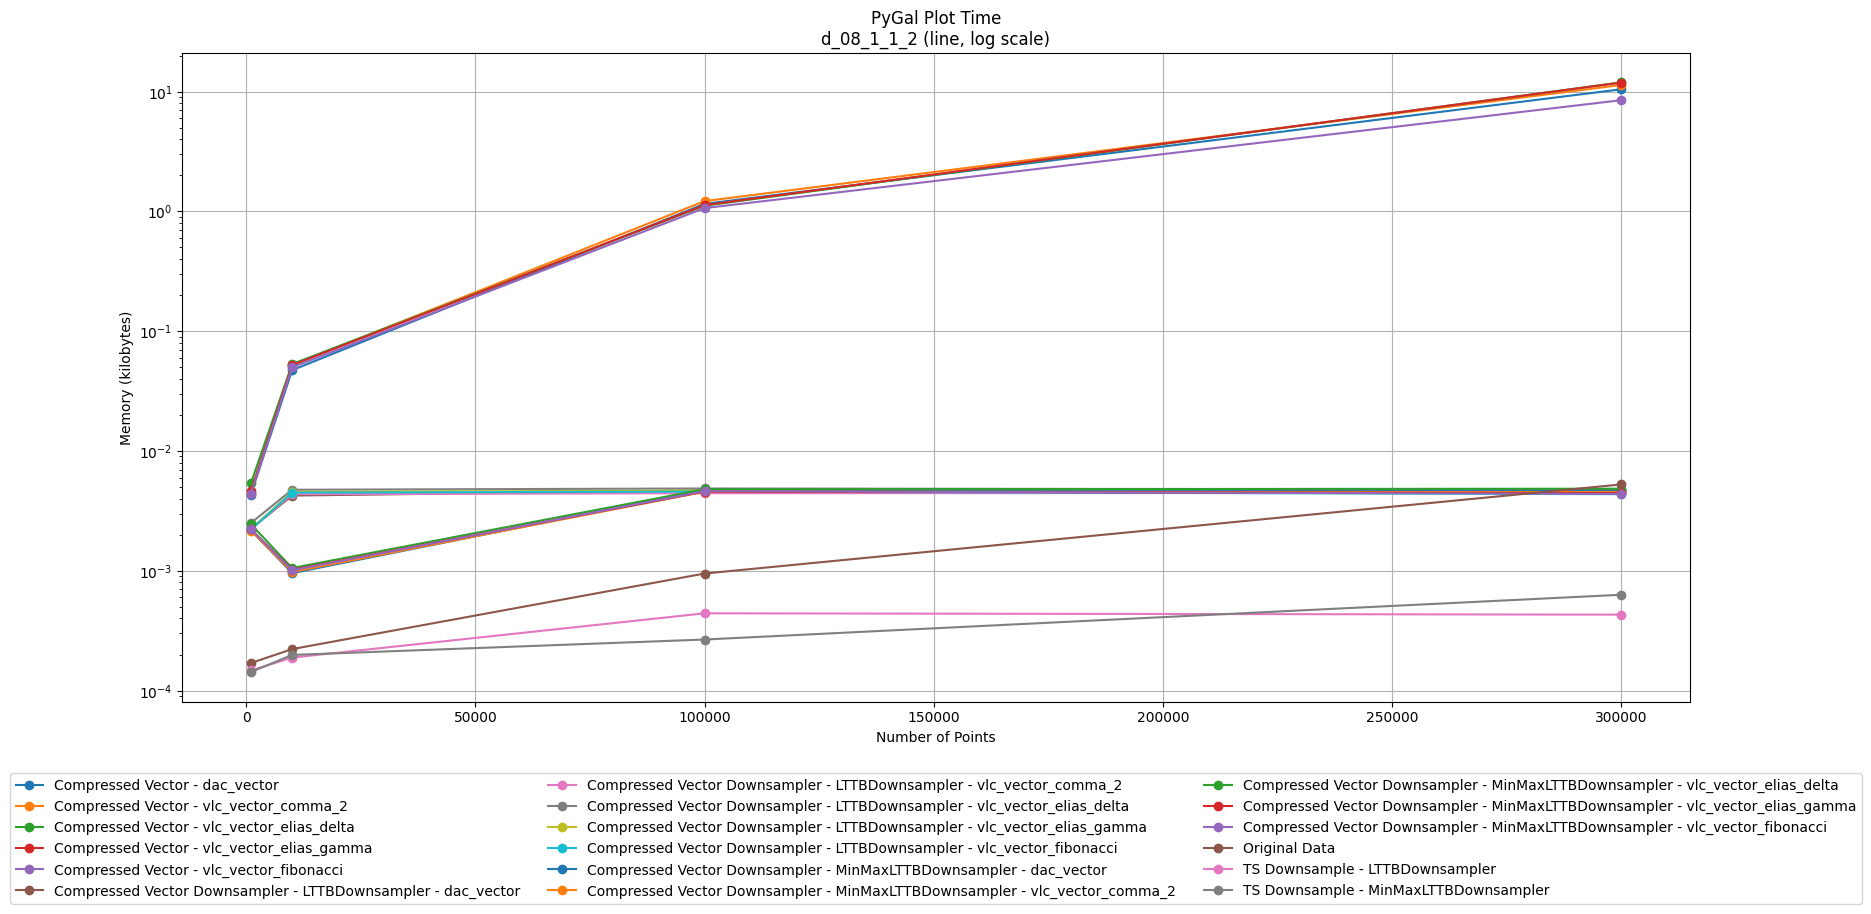
\includegraphics[width=1\textwidth]{anexo/exp/PyGal Plot Time/plots/PyGal Plot Time_d_08_1_1_2_log_line.png}
        \caption[]{Gráfico de tiempo de renderización PyGal para el input \textbf{d\_08\_1\_1\_2} en escala logarítmica.}
        \label{fig:pygal_plot_time_plot_line_1_log}
    \end{figure}
}

\DeclareRobustCommand{\PyGalPlotTimeOnePlotBar}{
    %insertar imagen
    \begin{figure}[H]
        \centering
        \includegraphics[width=1\textwidth]{anexo/exp/PyGal Plot Time/bar_plots/PyGal Plot Time_d_08_1_1_2_linear_bar.png}
        \caption[]{Gráfico de tiempo de renderización PyGal para el input \textbf{d\_08\_1\_1\_2}.}
        \label{fig:pygal_plot_time_plot_bar_1}
    \end{figure}
}

\DeclareRobustCommand{\PyGalPlotTimeTwoPlotLine}{
    %insertar imagen
    \begin{figure}[H]
        \centering
        \includegraphics[width=1\textwidth]{anexo/exp/PyGal Plot Time/plots/PyGal Plot Time_d_08_1_1_10_linear_line.png}
        \caption[]{Gráfico de tiempo de renderización PyGal para el input \textbf{d\_08\_1\_1\_10}.}
        \label{fig:pygal_plot_time_plot_line_2}
    \end{figure}
    \begin{figure}[H]
        \centering
        \includegraphics[width=1\textwidth]{anexo/exp/PyGal Plot Time/plots/PyGal Plot Time_d_08_1_1_10_log_line.png}
        \caption[]{Gráfico de tiempo de renderización PyGal para el input \textbf{d\_08\_1\_1\_10} en escala logarítmica.}
        \label{fig:pygal_plot_time_plot_line_2_log}
    \end{figure}
}

\DeclareRobustCommand{\PyGalPlotTimeTwoPlotBar}{
    %insertar imagen
    \begin{figure}[H]
        \centering
        \includegraphics[width=1\textwidth]{anexo/exp/PyGal Plot Time/bar_plots/PyGal Plot Time_d_08_1_1_10_linear_bar.png}
        \caption[]{Gráfico de tiempo de renderización PyGal para el input \textbf{d\_08\_1\_1\_10}.}
        \label{fig:pygal_plot_time_plot_bar_2}
    \end{figure}
}

\DeclareRobustCommand{\PyGalPlotTimeThreePlotLine}{
    %insertar imagen
    \begin{figure}[H]
        \centering
        \includegraphics[width=1\textwidth]{anexo/exp/PyGal Plot Time/plots/PyGal Plot Time_yellow_tripdata_2015-01_linear_line.png}
        \caption[]{Gráfico de tiempo de renderización PyGal para el input \textbf{yellow\_tripdata\_2015\_01}.}
        \label{fig:pygal_plot_time_plot_line_3}
    \end{figure}
    \begin{figure}[H]
        \centering
        \includegraphics[width=1\textwidth]{anexo/exp/PyGal Plot Time/plots/PyGal Plot Time_yellow_tripdata_2015-01_log_line.png}
        \caption[]{Gráfico de tiempo de renderización PyGal para el input \textbf{yellow\_tripdata\_2015\_01}.}
        \label{fig:pygal_plot_time_plot_line_3_log}
    \end{figure}
}

\DeclareRobustCommand{\PyGalPlotTimeThreePlotBar}{
    %insertar imagen
    \begin{figure}[H]
        \centering
        \includegraphics[width=1\textwidth]{anexo/exp/PyGal Plot Time/bar_plots/PyGal Plot Time_yellow_tripdata_2015-01_linear_bar.png}
        \caption[]{Gráfico de tiempo de renderización PyGal para el input \textbf{yellow\_tripdata\_2015\_01}.}
        \label{fig:pygal_plot_time_plot_bar_3}
    \end{figure}
}

\DeclareRobustCommand{\SDSLFourPyAccessTimeComparisonOnePlotBar}{
    \begin{figure}[H]
        \centering
        \includegraphics[width=1\textwidth]{anexo/exp/SDSL4Py Access Time Comparison/bar_plots/SDSL4Py Access Time Comparison_d_08_1_1_2_log_bar.png}
        \caption[]{Gráfico de tiempo de acceso SDSL4Py en escala logarítmica para el input \textbf{d\_08\_1\_1\_2}.}
        \label{fig:sdsl4py_access_time_comparison_plot_log_bar_1}
    \end{figure}
}

\DeclareRobustCommand{\SDSLFourPyAccessTimeComparisonTwoPlotBar}{
    \begin{figure}[H]
        \centering
        \includegraphics[width=1\textwidth]{anexo/exp/SDSL4Py Access Time Comparison/bar_plots/SDSL4Py Access Time Comparison_d_08_1_1_10_log_bar.png}
        \caption[]{Gráfico de tiempo de acceso SDSL4Py en escala logarítmica para el input \textbf{d\_08\_1\_1\_10}.}
        \label{fig:sdsl4py_access_time_comparison_plot_log_bar_2}
    \end{figure}
}

\DeclareRobustCommand{\SDSLFourPyAccessTimeComparisonThreePlotBar}{
    \begin{figure}[H]
        \centering
        \includegraphics[width=1\textwidth]{anexo/exp/SDSL4Py Access Time Comparison/bar_plots/SDSL4Py Access Time Comparison_yellow_tripdata_2015-01_log_bar.png}
        \caption[]{Gráfico de tiempo de acceso SDSL4Py en escala logarítmica para el input \textbf{yellow\_tripdata\_2015\_01}.}
        \label{fig:sdsl4py_access_time_comparison_plot_log_bar_3}
    \end{figure}
}

\DeclareRobustCommand{\SDSLFourPyCompressionSpaceComparisonOnePlotBar}{
    \begin{figure}[H]
        \centering
        \includegraphics[width=1\textwidth]{anexo/exp/SDSL4Py Compression Space Comparison/bar_plots/SDSL4Py Compression Space Comparison_d_08_1_1_2_log_bar.png}
        \caption[]{Gráfico de espacio de compresión SDSL4Py en escala logarítmica para el input \textbf{d\_08\_1\_1\_2}.}
        \label{fig:sdsl4py_compression_space_comparison_plot_log_bar_1}
    \end{figure}
}

\DeclareRobustCommand{\SDSLFourPyCompressionSpaceComparisonTwoPlotBar}{
    \begin{figure}[H]
        \centering
        \includegraphics[width=1\textwidth]{anexo/exp/SDSL4Py Compression Space Comparison/bar_plots/SDSL4Py Compression Space Comparison_d_08_1_1_10_log_bar.png}
        \caption[]{Gráfico de espacio de compresión SDSL4Py en escala logarítmica para el input \textbf{d\_08\_1\_1\_10}.}
        \label{fig:sdsl4py_compression_space_comparison_plot_log_bar_2}
    \end{figure}
}

\DeclareRobustCommand{\SDSLFourPyCompressionSpaceComparisonThreePlotBar}{
    \begin{figure}[H]
        \centering
        \includegraphics[width=1\textwidth]{anexo/exp/SDSL4Py Compression Space Comparison/bar_plots/SDSL4Py Compression Space Comparison_yellow_tripdata_2015-01_log_bar.png}
        \caption[]{Gráfico de espacio de compresión SDSL4Py en escala logarítmica para el input \textbf{yellow\_tripdata\_2015\_01}.}
        \label{fig:sdsl4py_compression_space_comparison_plot_log_bar_3}
    \end{figure}
}
\DeclareRobustCommand{\SDSLFourPyCompressionTimeComparisonOnePlotBar}{
    \begin{figure}[H]
        \centering
        \includegraphics[width=1\textwidth]{anexo/exp/SDSL4Py Compression Time Comparison/bar_plots/SDSL4Py Compression Time Comparison_d_08_1_1_2_log_bar.png}
        \caption[]{Gráfico de tiempo de compresión SDSL4Py en escala logarítmica para el input \textbf{d\_08\_1\_1\_2}.}
        \label{fig:sdsl4py_compression_time_comparison_plot_log_bar_1}
    \end{figure}
}

\DeclareRobustCommand{\SDSLFourPyCompressionTimeComparisonTwoPlotBar}{
    \begin{figure}[H]
        \centering
        \includegraphics[width=1\textwidth]{anexo/exp/SDSL4Py Compression Time Comparison/bar_plots/SDSL4Py Compression Time Comparison_d_08_1_1_10_log_bar.png}
        \caption[]{Gráfico de tiempo de compresión SDSL4Py en escala logarítmica para el input \textbf{d\_08\_1\_1\_10}.}
        \label{fig:sdsl4py_compression_time_comparison_plot_log_bar_2}
    \end{figure}
}

\DeclareRobustCommand{\SDSLFourPyCompressionTimeComparisonThreePlotBar}{
    \begin{figure}[H]
        \centering
        \includegraphics[width=1\textwidth]{anexo/exp/SDSL4Py Compression Time Comparison/bar_plots/SDSL4Py Compression Time Comparison_yellow_tripdata_2015-01_log_bar.png}
        \caption[]{Gráfico de tiempo de compresión SDSL4Py en escala logarítmica para el input \textbf{yellow\_tripdata\_2015\_01}.}
        \label{fig:sdsl4py_compression_time_comparison_plot_log_bar_3}
    \end{figure}
}


% Vega-Altair Plot Time Comparison
\DeclareRobustCommand{\VegaAltairPlotTimeComparisonOnePlotLine}{
    %insertar imagen
    \begin{figure}[H]
        \centering
        \includegraphics[width=1\textwidth]{anexo/exp/Vega-Altair Plot Time Comparison/plots/Vega-Altair Plot Time Comparison_d_08_1_1_2_linear_line.png}
        \caption[]{Gráfico de tiempo de renderización Vega-Altair para el input \textbf{d\_08\_1\_1\_2}.}
        \label{fig:vega_altair_plot_time_comparison_plot_line_1}
    \end{figure}
    \begin{figure}[H]
        \centering
        \includegraphics[width=1\textwidth]{anexo/exp/Vega-Altair Plot Time Comparison/plots/Vega-Altair Plot Time Comparison_d_08_1_1_2_log_line.png}
        \caption[]{Gráfico de tiempo de renderización Vega-Altair para el input \textbf{d\_08\_1\_1\_2} en escala logarítmica.}
        \label{fig:vega_altair_plot_time_comparison_plot_line_1}
    \end{figure}
}

\DeclareRobustCommand{\VegaAltairPlotTimeComparisonOnePlotBar}{
    %insertar imagen
    \begin{figure}[H]
        \centering
        \includegraphics[width=1\textwidth]{anexo/exp/Vega-Altair Plot Time Comparison/bar_plots/Vega-Altair Plot Time Comparison_d_08_1_1_2_linear_bar.png}
        \caption[]{Gráfico de tiempo de renderización Vega-Altair para el input \textbf{d\_08\_1\_1\_2}.}
        \label{fig:vega_altair_plot_time_comparison_plot_bar_1}
    \end{figure}
}

\DeclareRobustCommand{\VegaAltairPlotTimeComparisonTwoPlotLine}{
    %insertar imagen
    \begin{figure}[H]
        \centering
        \includegraphics[width=1\textwidth]{anexo/exp/Vega-Altair Plot Time Comparison/plots/Vega-Altair Plot Time Comparison_d_08_1_1_10_linear_line.png}
        \caption[]{Gráfico de tiempo de renderización Vega-Altair para el input \textbf{d\_08\_1\_1\_10}.}
        \label{fig:vega_altair_plot_time_comparison_plot_line_2}
    \end{figure}
}

\DeclareRobustCommand{\VegaAltairPlotTimeComparisonTwoPlotBar}{
    %insertar imagen
    \begin{figure}[H]
        \centering
        \includegraphics[width=1\textwidth]{anexo/exp/Vega-Altair Plot Time Comparison/bar_plots/Vega-Altair Plot Time Comparison_d_08_1_1_10_linear_bar.png}
        \caption[]{Gráfico de tiempo de renderización Vega-Altair para el input \textbf{d\_08\_1\_1\_10}.}
        \label{fig:vega_altair_plot_time_comparison_plot_bar_2}
    \end{figure}
}

\DeclareRobustCommand{\VegaAltairPlotTimeComparisonThreePlotLine}{
    %insertar imagen
    \begin{figure}[H]
        \centering
        \includegraphics[width=1\textwidth]{anexo/exp/Vega-Altair Plot Time Comparison/plots/Vega-Altair Plot Time Comparison_yellow_tripdata_2015-01_linear_line.png}
        \caption[]{Gráfico de tiempo de renderización Vega-Altair para el input \textbf{yellow\_tripdata\_2015\_01}.}
        \label{fig:vega_altair_plot_time_comparison_plot_line_3}
    \end{figure}
}

\DeclareRobustCommand{\VegaAltairPlotTimeComparisonThreePlotBar}{
    %insertar imagen
    \begin{figure}[H]
        \centering
        \includegraphics[width=1\textwidth]{anexo/exp/Vega-Altair Plot Time Comparison/bar_plots/Vega-Altair Plot Time Comparison_yellow_tripdata_2015-01_linear_bar.png}
        \caption[]{Gráfico de tiempo de renderización Vega-Altair para el input \textbf{yellow\_tripdata\_2015\_01}.}
        \label{fig:vega_altair_plot_time_comparison_plot_bar_3}
    \end{figure}
}

% Vega-Altair Plotting + Building Comparison
\DeclareRobustCommand{\VegaAltairPlottingBuildingComparisonOnePlotLine}{
    %insertar imagen
    \begin{figure}[H]
        \centering
        \includegraphics[width=1\textwidth]{anexo/exp/Vega-Altair Plotting + Building Comparison/plots/Vega-Altair Plotting + Building Comparison_d_08_1_1_2_linear_line.png}
        \caption[]{Gráfico de tiempo de renderización y construcción Vega-Altair para el input \textbf{d\_08\_1\_1\_2}.}
        \label{fig:vega_altair_plotting_building_comparison_plot_line_1}
    \end{figure}
}

\DeclareRobustCommand{\VegaAltairPlottingBuildingComparisonOnePlotBar}{
    %insertar imagen
    \begin{figure}[H]
        \centering
        \includegraphics[width=1\textwidth]{anexo/exp/Vega-Altair Plotting + Building Comparison/bar_plots/Vega-Altair Plotting + Building Comparison_d_08_1_1_2_linear_bar.png}
        \caption[]{Gráfico de tiempo de renderización y construcción Vega-Altair para el input \textbf{d\_08\_1\_1\_2}.}
        \label{fig:vega_altair_plotting_building_comparison_plot_bar_1}
    \end{figure}
}

\DeclareRobustCommand{\VegaAltairPlottingBuildingComparisonTwoPlotLine}{
    %insertar imagen
    \begin{figure}[H]
        \centering
        \includegraphics[width=1\textwidth]{anexo/exp/Vega-Altair Plotting + Building Comparison/plots/Vega-Altair Plotting + Building Comparison_d_08_1_1_10_linear_line.png}
        \caption[]{Gráfico de tiempo de renderización y construcción Vega-Altair para el input \textbf{d\_08\_1\_1\_10}.}
        \label{fig:vega_altair_plotting_building_comparison_plot_line_2}
    \end{figure}
}

\DeclareRobustCommand{\VegaAltairPlottingBuildingComparisonTwoPlotBar}{
    %insertar imagen
    \begin{figure}[H]
        \centering
        \includegraphics[width=1\textwidth]{anexo/exp/Vega-Altair Plotting + Building Comparison/bar_plots/Vega-Altair Plotting + Building Comparison_d_08_1_1_10_linear_bar.png}
        \caption[]{Gráfico de tiempo de renderización y construcción Vega-Altair para el input \textbf{d\_08\_1\_1\_10}.}
        \label{fig:vega_altair_plotting_building_comparison_plot_bar_2}
    \end{figure}
}

\DeclareRobustCommand{\VegaAltairPlottingBuildingComparisonThreePlotLine}{
    %insertar imagen
    \begin{figure}[H]
        \centering
        \includegraphics[width=1\textwidth]{anexo/exp/Vega-Altair Plotting + Building Comparison/plots/Vega-Altair Plotting + Building Comparison_yellow_tripdata_2015-01_linear_line.png}
        \caption[]{Gráfico de tiempo de renderización y construcción Vega-Altair para el input \textbf{yellow\_tripdata\_2015\_01}.}
        \label{fig:vega_altair_plotting_building_comparison_plot_line_3}
    \end{figure}
}

\DeclareRobustCommand{\VegaAltairPlottingBuildingComparisonThreePlotBar}{
    %insertar imagen
    \begin{figure}[H]
        \centering
        \includegraphics[width=1\textwidth]{anexo/exp/Vega-Altair Plotting + Building Comparison/bar_plots/Vega-Altair Plotting + Building Comparison_yellow_tripdata_2015-01_linear_bar.png}
        \caption[]{Gráfico de tiempo de renderización y construcción Vega-Altair para el input \textbf{yellow\_tripdata\_2015\_01}.}
        \label{fig:vega_altair_plotting_building_comparison_plot_bar_3}
    \end{figure}
}

% VEGA ALTAIR MEMORY ALLOCATION

\DeclareRobustCommand{\VegaAltairMemoryAllocationOnePlotLine}{
    %insertar imagen
    \begin{figure}[H]
        \centering
        \includegraphics[width=1\textwidth]{anexo/exp/Vega-Altair Plotting Memory Allocation/plots/Vega-Altair Plotting Memory Allocation_d_08_1_1_2_log_line.png}
        \caption[]{Gráfico de tiempo de renderización y construcción Vega-Altair para el input \textbf{d\_08\_1\_1\_2}.}
        \label{fig:vega_altair_plotting_building_comparison_plot_line_1}
    \end{figure}
}

\DeclareRobustCommand{\VegaAltairMemoryAllocationOnePlotBar}{
    %insertar imagen
    \begin{figure}[H]
        \centering
        \includegraphics[width=1\textwidth]{anexo/exp/Vega-Altair Plotting Memory Allocation/bar_plots/Vega-Altair Plotting Memory Allocation_d_08_1_1_2_log_bar.png}
        \caption[]{Gráfico de tiempo de renderización y construcción Vega-Altair para el input \textbf{d\_08\_1\_1\_2}.}
        \label{fig:vega_altair_plotting_building_comparison_plot_bar_1}
    \end{figure}
\begin{table}[H]
\centering
\caption{\textit{d\_08\_1\_1\_2} – Memoria por elemento [KB]}
\label{tab:Vega-Altair Plotting Memory Allocation\_d\_08\_1\_1\_2_mem_por_elemento_sin_original}
\begin{tabular}{rrrr}
\toprule
 & CVD - dac\_vector & CVD - vlc\_vector\_fibonacci & TS Downsample \\
n\_size &  &  &  \\
\midrule
6000 & 0.16 & 0.16 & 0.16 \\
12000 & 0.16 & 0.16 & 0.16 \\
20000 & 0.17 & 0.17 & 0.16 \\
70000 & 0.18 & 0.18 & 0.17 \\
100000 & 0.18 & 0.18 & 0.17 \\
300000 & 0.19 & 0.18 & 0.17 \\
\bottomrule
\end{tabular}

\end{table}
}

\DeclareRobustCommand{\VegaAltairMemoryAllocationTwoPlotLine}{
    %insertar imagen
    \begin{figure}[H]
        \centering
        \includegraphics[width=1\textwidth]{anexo/exp/Vega-Altair Plotting Memory Allocation/plots/Vega-Altair Plotting Memory Allocation_d_08_1_1_10_log_line.png}
        \caption[]{Gráfico de tiempo de renderización y construcción Vega-Altair para el input \textbf{d\_08\_1\_1\_10}.}
        \label{fig:vega_altair_plotting_building_comparison_plot_line_2}
    \end{figure}
}

\DeclareRobustCommand{\VegaAltairMemoryAllocationTwoPlotBar}{
    %insertar imagen
    \begin{figure}[H]
        \centering
        \includegraphics[width=1\textwidth]{anexo/exp/Vega-Altair Plotting Memory Allocation/bar_plots/Vega-Altair Plotting Memory Allocation_d_08_1_1_10_log_bar.png}
        \caption[]{Gráfico de asignación de memoria con la biblioteca Vega-Altair para el input \textbf{d\_08\_1\_1\_10}.}
        \label{fig:vega_altair_plotting_building_comparison_plot_bar_2}
    \end{figure}
\begin{table}[H]
\centering
\caption{\textit{d\_08\_1\_1\_10} – Memoria por elemento [KB]}
\label{tab:Vega-Altair Plotting Memory Allocation\_d\_08\_1\_1\_10_mem_por_elemento_sin_original}
\begin{tabular}{rrrr}
\toprule
 & CVD - dac\_vector & CVD - vlc\_vector\_fibonacci & TS Downsample \\
n\_size &  &  &  \\
\midrule
6000 & 0.16 & 0.16 & 0.16 \\
12000 & 0.16 & 0.16 & 0.16 \\
20000 & 0.17 & 0.17 & 0.16 \\
70000 & 0.18 & 0.18 & 0.17 \\
100000 & 0.18 & 0.18 & 0.17 \\
300000 & 0.18 & 0.20 & 0.17 \\
\bottomrule
\end{tabular}

\end{table}
}

\DeclareRobustCommand{\VegaAltairMemoryAllocationThreePlotLine}{
    %insertar imagen
    \begin{figure}[H]
        \centering
        \includegraphics[width=1\textwidth]{anexo/exp/Vega-Altair Plotting Memory Allocation/plots/Vega-Altair Plotting Memory Allocation_yellow_tripdata_2015-01_log_line.png}
        \caption[]{Gráfico de asignación de memoria con la biblioteca Vega-Altair para el input \textbf{yellow\_tripdata\_2015\_01}.}
        \label{fig:vega_altair_plotting_building_comparison_plot_line_3}
    \end{figure}
}

\DeclareRobustCommand{\VegaAltairMemoryAllocationThreePlotBar}{
    %insertar imagen
    \begin{figure}[H]
        \centering
        \includegraphics[width=1\textwidth]{anexo/exp/Vega-Altair Plotting Memory Allocation/bar_plots/Vega-Altair Plotting Memory Allocation_yellow_tripdata_2015-01_log_bar.png}
        \caption[]{Gráfico de asignación de memoria con la biblioteca Vega-Altair para el input \textbf{yellow\_tripdata\_2015\_01}.}
        \label{fig:vega_altair_plotting_building_comparison_plot_bar_3}
    \end{figure}
\begin{table}[H]
\centering
\caption{\textit{yellow\_tripdata\_2015-01} – Memoria por elemento [KB]}
\label{tab:Vega-Altair Plotting Memory Allocation\_yellow\_tripdata\_2015-01_mem_por_elemento_sin_original}
\begin{tabular}{rrrr}
\toprule
 & CVD - dac\_vector & CVD - vlc\_vector\_fibonacci & TS Downsample \\
n\_size &  &  &  \\
\midrule
6000 & 0.16 & 0.16 & 0.16 \\
12000 & 0.16 & 0.16 & 0.16 \\
20000 & 0.16 & 0.16 & 0.16 \\
70000 & 0.16 & 0.16 & 0.16 \\
100000 & 0.16 & 0.16 & 0.16 \\
300000 & 0.16 & 0.16 & 0.16 \\
\bottomrule
\end{tabular}

\end{table}
}

% All Libraries Memory Allocation

\DeclareRobustCommand{\AllLibrariesMemoryAllocationOneTable}
{
    \vspace{0.5em}
    \input{anexo/exp/All Libraries Memory Allocation/txts/All Libraries Memory Allocation_d_08_1_1_2.txt}
}
\DeclareRobustCommand{\AllLibrariesMemoryAllocationTwoTable}
{
    \vspace{0.5em}
    \input{anexo/exp/All Libraries Memory Allocation/txts/All Libraries Memory Allocation_d_08_1_1_2_10.txt}
}
\DeclareRobustCommand{\AllLibrariesMemoryAllocationThreeTable}
{
    \vspace{0.5em}
    \input{anexo/exp/All Libraries Memory Allocation/txts/All Libraries Memory Allocation_yellow_tripdata_2015-01.txt}
}

% All Libraries Time Comparison
\DeclareRobustCommand{\AllLibrariesTimeComparisonOneTable}
{
    \vspace{0.5em}
    \input{anexo/exp/All Libraries Time Comparison/txts/All Libraries Time Comparison_d_08_1_1_2.txt}
}
\DeclareRobustCommand{\AllLibrariesTimeComparisonTwoTable}
{
    \vspace{0.5em}
    \input{anexo/exp/All Libraries Time Comparison/txts/All Libraries Time Comparison_d_08_1_1_2_10.txt}
}
\DeclareRobustCommand{\AllLibrariesTimeComparisonThreeTable}
{
    \vspace{0.5em}
    \input{anexo/exp/All Libraries Time Comparison/txts/All Libraries Time Comparison_yellow_tripdata_2015-01.txt}
}

% Building Time Comparison
\DeclareRobustCommand{\BuildingTimeComparisonOneTable}
{
    \vspace{0.5em}
    \input{anexo/exp/Building Time Comparison/txts/Building Time Comparison_d_08_1_1_2.txt}
}
\DeclareRobustCommand{\BuildingTimeComparisonTwoTable}
{
    \vspace{0.5em}
    \input{anexo/exp/Building Time Comparison/txts/Building Time Comparison_d_08_1_1_2_10.txt}
}
\DeclareRobustCommand{\BuildingTimeComparisonThreeTable}
{
    \vspace{0.5em}
    \input{anexo/exp/Building Time Comparison/txts/Building Time Comparison_yellow_tripdata_2015-01.txt}
}

% Comparison of Space Used
\DeclareRobustCommand{\ComparisonOfSpaceUsedOneTable}
{
    \vspace{0.5em}
    \input{anexo/exp/Comparison of Space Used/txts/Comparison of Space Used_d_08_1_1_2.txt}
}
\DeclareRobustCommand{\ComparisonOfSpaceUsedTwoTable}
{
    \vspace{0.5em}
    \input{anexo/exp/Comparison of Space Used/txts/Comparison of Space Used_d_08_1_1_2_10.txt}
}
\DeclareRobustCommand{\ComparisonOfSpaceUsedThreeTable}
{
    \vspace{0.5em}
    \input{anexo/exp/Comparison of Space Used/txts/Comparison of Space Used_yellow_tripdata_2015-01.txt}
}

% CVD Decimal Places Access Time Comparison
\DeclareRobustCommand{\CVDDecimalPlacesAccessTimeComparisonOneTable}
{
    \vspace{0.5em}
    \input{anexo/exp/CVD Decimal Places Access Time Comparison/txts/CVD Decimal Places Access Time Comparison_d_08_1_1_2.txt}
}
\DeclareRobustCommand{\CVDDecimalPlacesAccessTimeComparisonTwoTable}
{
    \vspace{0.5em}
    \input{anexo/exp/CVD Decimal Places Access Time Comparison/txts/CVD Decimal Places Access Time Comparison_d_08_1_1_10.txt}
}
\DeclareRobustCommand{\CVDDecimalPlacesAccessTimeComparisonThreeTable}
{
    \vspace{0.5em}
    \input{anexo/exp/CVD Decimal Places Access Time Comparison/txts/CVD Decimal Places Access Time Comparison_yellow_tripdata_2015-01.txt}
}

% CVD Decimal Places Build Time Comparison
\DeclareRobustCommand{\CVDDecimalPlacesBuildTimeComparisonOneTable}
{
    \vspace{0.5em}
    \input{anexo/exp/CVD Decimal Places Build Time Comparison/txts/CVD Decimal Places Build Time Comparison_d_08_1_1_2.txt}
}
\DeclareRobustCommand{\CVDDecimalPlacesBuildTimeComparisonTwoTable}
{
    \vspace{0.5em}
    \input{anexo/exp/CVD Decimal Places Build Time Comparison/txts/CVD Decimal Places Build Time Comparison_d_08_1_1_10.txt}
}
\DeclareRobustCommand{\CVDDecimalPlacesBuildTimeComparisonThreeTable}
{
    \vspace{0.5em}
    \input{anexo/exp/CVD Decimal Places Build Time Comparison/txts/CVD Decimal Places Build Time Comparison_yellow_tripdata_2015-01.txt}
}

% CVD Decimal Places Size Comparison
\DeclareRobustCommand{\CVDDecimalPlacesSizeComparisonOneTable}
{
    \vspace{0.5em}
    \input{anexo/exp/CVD Decimal Places Size Comparison/txts/CVD Decimal Places Size Comparison_d_08_1_1_2.txt}
}
\DeclareRobustCommand{\CVDDecimalPlacesSizeComparisonTwoTable}
{
    \vspace{0.5em}
    \input{anexo/exp/CVD Decimal Places Size Comparison/txts/CVD Decimal Places Size Comparison_d_08_1_1_10.txt}
}
\DeclareRobustCommand{\CVDDecimalPlacesSizeComparisonThreeTable}
{
    \vspace{0.5em}
    \input{anexo/exp/CVD Decimal Places Size Comparison/txts/CVD Decimal Places Size Comparison_yellow_tripdata_2015-01.txt}
}

% PyGal Memory Allocation
\DeclareRobustCommand{\PyGalMemoryAllocationOneTable}
{
    \vspace{0.5em}
    \input{anexo/exp/PyGal Memory Allocation/txts/PyGal Memory Allocation_d_08_1_1_2.txt}
}
\DeclareRobustCommand{\PyGalMemoryAllocationTwoTable}
{
    \vspace{0.5em}
    \input{anexo/exp/PyGal Memory Allocation/txts/PyGal Memory Allocation_d_08_1_1_10.txt}
}
\DeclareRobustCommand{\PyGalMemoryAllocationThreeTable}
{
    \vspace{0.5em}
    \input{anexo/exp/PyGal Memory Allocation/txts/PyGal Memory Allocation_yellow_tripdata_2015-01.txt}
}

% PyGal Plot Time
\DeclareRobustCommand{\PyGalPlotTimeOneTable}
{
    \vspace{0.5em}
    \input{anexo/exp/PyGal Plot Time/txts/PyGal Plot Time_d_08_1_1_2.txt}
}
\DeclareRobustCommand{\PyGalPlotTimeTwoTable}
{
    \vspace{0.5em}
    \input{anexo/exp/PyGal Plot Time/txts/PyGal Plot Time_d_08_1_1_10.txt}
}
\DeclareRobustCommand{\PyGalPlotTimeThreeTable}
{
    \vspace{0.5em}
    \input{anexo/exp/PyGal Plot Time/txts/PyGal Plot Time_yellow_tripdata_2015-01.txt}
}

% SDSL4Py Access Time Comparison
\DeclareRobustCommand{\SDSLFourPyAccessTimeComparisonOneTable}
{
    \vspace{0.5em}
    \input{anexo/exp/SDSL4Py Access Time Comparison/txts/SDSL4Py Access Time Comparison_d_08_1_1_2.txt}
}
\DeclareRobustCommand{\SDSLFourPyAccessTimeComparisonTwoTable}
{
    \vspace{0.5em}
    \input{anexo/exp/SDSL4Py Access Time Comparison/txts/SDSL4Py Access Time Comparison_d_08_1_1_10.txt}
}
\DeclareRobustCommand{\SDSLFourPyAccessTimeComparisonThreeTable}
{
    \vspace{0.5em}
    \input{anexo/exp/SDSL4Py Access Time Comparison/txts/SDSL4Py Access Time Comparison_yellow_tripdata_2015-01.txt}
}

% SDSL4Py Compression Space Comparison
\DeclareRobustCommand{\SDSLFourPyCompressionSpaceComparisonOneTable}
{
    \vspace{0.5em}
    \input{anexo/exp/SDSL4Py Compression Space Comparison/txts/SDSL4Py Compression Space Comparison_d_08_1_1_2.txt}
}
\DeclareRobustCommand{\SDSLFourPyCompressionSpaceComparisonTwoTable}
{
    \vspace{0.5em}
    \input{anexo/exp/SDSL4Py Compression Space Comparison/txts/SDSL4Py Compression Space Comparison_d_08_1_1_10.txt}
}
\DeclareRobustCommand{\SDSLFourPyCompressionSpaceComparisonThreeTable}
{
    \vspace{0.5em}
    \input{anexo/exp/SDSL4Py Compression Space Comparison/txts/SDSL4Py Compression Space Comparison_yellow_tripdata_2015-01.txt}
}

% SDSL4Py Compression Time Comparison
\DeclareRobustCommand{\SDSLFourPyCompressionTimeComparisonOneTable}
{
    \vspace{0.5em}
    \input{anexo/exp/SDSL4Py Compression Time Comparison/txts/SDSL4Py Compression Time Comparison_d_08_1_1_2.txt}
}
\DeclareRobustCommand{\SDSLFourPyCompressionTimeComparisonTwoTable}
{
    \vspace{0.5em}
    \input{anexo/exp/SDSL4Py Compression Time Comparison/txts/SDSL4Py Compression Time Comparison_d_08_1_1_10.txt}
}
\DeclareRobustCommand{\SDSLFourPyCompressionTimeComparisonThreeTable}
{
    \vspace{0.5em}
    \input{anexo/exp/SDSL4Py Compression Time Comparison/txts/SDSL4Py Compression Time Comparison_yellow_tripdata_2015-01.txt}
}

% Vega-Altair Plot Time Comparison
\DeclareRobustCommand{\VegaAltairPlotTimeComparisonOneTable}
{
    \vspace{0.5em}
    \input{anexo/exp/Vega-Altair Plot Time Comparison/txts/Vega-Altair Plot Time Comparison_d_08_1_1_2.txt}
}
\DeclareRobustCommand{\VegaAltairPlotTimeComparisonTwoTable}
{
    \vspace{0.5em}
    \input{anexo/exp/Vega-Altair Plot Time Comparison/txts/Vega-Altair Plot Time Comparison_d_08_1_1_10.txt}
}
\DeclareRobustCommand{\VegaAltairPlotTimeComparisonThreeTable}
{
    \vspace{0.5em}
    \input{anexo/exp/Vega-Altair Plot Time Comparison/txts/Vega-Altair Plot Time Comparison_yellow_tripdata_2015-01.txt}
}

% Vega-Altair Plotting + Building Comparison
\DeclareRobustCommand{\VegaAltairPlottingBuildingComparisonOneTable}
{
    \vspace{0.5em}
    \input{anexo/exp/Vega-Altair Plotting + Building Comparison/txts/Vega-Altair Plotting + Building Comparison_d_08_1_1_2.txt}
}
\DeclareRobustCommand{\VegaAltairPlottingBuildingComparisonTwoTable}
{
    \vspace{0.5em}
    \input{anexo/exp/Vega-Altair Plotting + Building Comparison/txts/Vega-Altair Plotting + Building Comparison_d_08_1_1_10.txt}
}
\DeclareRobustCommand{\VegaAltairPlottingBuildingComparisonThreeTable}
{
    \vspace{0.5em}
    \input{anexo/exp/Vega-Altair Plotting + Building Comparison/txts/Vega-Altair Plotting + Building Comparison_yellow_tripdata_2015-01.txt}
}

\DeclareRobustCommand{\AllLibrariesMemoryAllocation}
{
    \AllLibrariesMemoryAllocationOnePlotBar
    \AllLibrariesMemoryAllocationOnePlotLine
    \AllLibrariesMemoryAllocationOneTable

    \AllLibrariesMemoryAllocationTwoPlotBar
    \AllLibrariesMemoryAllocationTwoPlotLine
    \AllLibrariesMemoryAllocationTwoTable

    \AllLibrariesMemoryAllocationThreePlotBar
    \AllLibrariesMemoryAllocationThreePlotLine
    \AllLibrariesMemoryAllocationThreeTable
}

\DeclareRobustCommand{\AllLibrariesTimeComparison}
{
    \AllLibrariesTimeComparisonOnePlotBar
    \AllLibrariesTimeComparisonOnePlotLine
    \AllLibrariesTimeComparisonOneTable

    \AllLibrariesTimeComparisonTwoPlotBar
    \AllLibrariesTimeComparisonTwoPlotLine
    \AllLibrariesTimeComparisonTwoTable
    
    \AllLibrariesTimeComparisonThreePlotBar
    \AllLibrariesTimeComparisonThreePlotLine
    \AllLibrariesTimeComparisonThreeTable
}

\DeclareRobustCommand{\BuildingTimeComparison}
{
    \BuildingTimeComparisonOnePlotBar
    \BuildingTimeComparisonOnePlotLine
    \BuildingTimeComparisonOneTable

    \BuildingTimeComparisonTwoPlotBar
    \BuildingTimeComparisonTwoPlotLine
    \BuildingTimeComparisonTwoTable
    
    \BuildingTimeComparisonThreePlotBar
    \BuildingTimeComparisonThreePlotLine
    \BuildingTimeComparisonThreeTable
}

\DeclareRobustCommand{\ComparisonOfSpaceUsed}
{
    \ComparisonOfSpaceUsedOnePlotBar
    \ComparisonOfSpaceUsedOnePlotLine
    \ComparisonOfSpaceUsedOneTable

    \ComparisonOfSpaceUsedTwoPlotBar
    \ComparisonOfSpaceUsedTwoPlotLine
    \ComparisonOfSpaceUsedTwoTable
    
    \ComparisonOfSpaceUsedThreePlotBar
    \ComparisonOfSpaceUsedThreePlotLine
    \ComparisonOfSpaceUsedThreeTable
}

\DeclareRobustCommand{\CVDDecimalPlacesAccessTimeComparison}
{
    \CVDDecimalPlacesAccessTimeComparisonOnePlotBar
    \CVDDecimalPlacesAccessTimeComparisonOnePlotLine
    \CVDDecimalPlacesAccessTimeComparisonOneTable

    \CVDDecimalPlacesAccessTimeComparisonTwoPlotBar
    \CVDDecimalPlacesAccessTimeComparisonTwoPlotLine
    \CVDDecimalPlacesAccessTimeComparisonTwoTable
    
    \CVDDecimalPlacesAccessTimeComparisonThreePlotBar
    \CVDDecimalPlacesAccessTimeComparisonThreePlotLine
    \CVDDecimalPlacesAccessTimeComparisonThreeTable
}

\DeclareRobustCommand{\CVDDecimalPlacesBuildTimeComparison}
{
    \CVDDecimalPlacesBuildTimeComparisonOnePlotBar
    \CVDDecimalPlacesBuildTimeComparisonOnePlotLine
    \CVDDecimalPlacesBuildTimeComparisonOneTable

    \CVDDecimalPlacesBuildTimeComparisonTwoPlotBar
    \CVDDecimalPlacesBuildTimeComparisonTwoPlotLine
    \CVDDecimalPlacesBuildTimeComparisonTwoTable
    
    \CVDDecimalPlacesBuildTimeComparisonThreePlotBar
    \CVDDecimalPlacesBuildTimeComparisonThreePlotLine
    \CVDDecimalPlacesBuildTimeComparisonThreeTable
}

\DeclareRobustCommand{\CVDDecimalPlacesSizeComparison}
{
    \CVDDecimalPlacesSizeComparisonOnePlotBar
    \CVDDecimalPlacesSizeComparisonOnePlotLine
    \CVDDecimalPlacesSizeComparisonOneTable

    \CVDDecimalPlacesSizeComparisonTwoPlotBar
    \CVDDecimalPlacesSizeComparisonTwoPlotLine
    \CVDDecimalPlacesSizeComparisonTwoTable
    
    \CVDDecimalPlacesSizeComparisonThreePlotBar
    \CVDDecimalPlacesSizeComparisonThreePlotLine
    \CVDDecimalPlacesSizeComparisonThreeTable
}

\DeclareRobustCommand{\PyGalMemoryAllocation}
{
    \PyGalMemoryAllocationOnePlotBar
    \PyGalMemoryAllocationOnePlotLine
    \PyGalMemoryAllocationOneTable

    \PyGalMemoryAllocationTwoPlotBar
    \PyGalMemoryAllocationTwoPlotLine
    \PyGalMemoryAllocationTwoTable
    
    \PyGalMemoryAllocationThreePlotBar
    \PyGalMemoryAllocationThreePlotLine
    \PyGalMemoryAllocationThreeTable
}

\DeclareRobustCommand{\PyGalPlotTime}
{
    \PyGalPlotTimeOnePlotBar
    \PyGalPlotTimeOnePlotLine
    \PyGalPlotTimeOneTable

    \PyGalPlotTimeTwoPlotBar
    \PyGalPlotTimeTwoPlotLine
    \PyGalPlotTimeTwoTable
    
    \PyGalPlotTimeThreePlotBar
    \PyGalPlotTimeThreePlotLine
    \PyGalPlotTimeThreeTable
}

\DeclareRobustCommand{\SDSLFourPyAccessTimeComparison}
{
    \SDSLFourPyAccessTimeComparisonOnePlotBar
    \SDSLFourPyAccessTimeComparisonOnePlotLine
    \SDSLFourPyAccessTimeComparisonOneTable

    \SDSLFourPyAccessTimeComparisonTwoPlotBar
    \SDSLFourPyAccessTimeComparisonTwoPlotLine
    \SDSLFourPyAccessTimeComparisonTwoTable
    
    \SDSLFourPyAccessTimeComparisonThreePlotBar
    \SDSLFourPyAccessTimeComparisonThreePlotLine
    \SDSLFourPyAccessTimeComparisonThreeTable
}

\DeclareRobustCommand{\SDSLFourPyCompressionSpaceComparison}
{
    \SDSLFourPyCompressionSpaceComparisonOnePlotBar
    \SDSLFourPyCompressionSpaceComparisonOnePlotLine
    \SDSLFourPyCompressionSpaceComparisonOneTable

    \SDSLFourPyCompressionSpaceComparisonTwoPlotBar
    \SDSLFourPyCompressionSpaceComparisonTwoPlotLine
    \SDSLFourPyCompressionSpaceComparisonTwoTable
    
    \SDSLFourPyCompressionSpaceComparisonThreePlotBar
    \SDSLFourPyCompressionSpaceComparisonThreePlotLine
    \SDSLFourPyCompressionSpaceComparisonThreeTable
}

\DeclareRobustCommand{\SDSLFourPyCompressionTimeComparison}
{
    \SDSLFourPyCompressionTimeComparisonOnePlotBar
    \SDSLFourPyCompressionTimeComparisonOnePlotLine
    \SDSLFourPyCompressionTimeComparisonOneTable

    \SDSLFourPyCompressionTimeComparisonTwoPlotBar
    \SDSLFourPyCompressionTimeComparisonTwoPlotLine
    \SDSLFourPyCompressionTimeComparisonTwoTable
    
    \SDSLFourPyCompressionTimeComparisonThreePlotBar
    \SDSLFourPyCompressionTimeComparisonThreePlotLine
    \SDSLFourPyCompressionTimeComparisonThreeTable
}

\DeclareRobustCommand{\VegaAltairPlotTimeComparison}
{
    \VegaAltairPlotTimeComparisonOnePlotBar
    \VegaAltairPlotTimeComparisonOnePlotLine
    \VegaAltairPlotTimeComparisonOneTable

    \VegaAltairPlotTimeComparisonTwoPlotBar
    \VegaAltairPlotTimeComparisonTwoPlotLine
    \VegaAltairPlotTimeComparisonTwoTable
    
    \VegaAltairPlotTimeComparisonThreePlotBar
    \VegaAltairPlotTimeComparisonThreePlotLine
    \VegaAltairPlotTimeComparisonThreeTable
}

\DeclareRobustCommand{\VegaAltairPlottingBuildingComparison}
{
    \VegaAltairPlottingBuildingComparisonOnePlotBar
    \VegaAltairPlottingBuildingComparisonOnePlotLine
    \VegaAltairPlottingBuildingComparisonOneTable

    \VegaAltairPlottingBuildingComparisonTwoPlotBar
    \VegaAltairPlottingBuildingComparisonTwoPlotLine
    \VegaAltairPlottingBuildingComparisonTwoTable
    
    \VegaAltairPlottingBuildingComparisonThreePlotBar
    \VegaAltairPlottingBuildingComparisonThreePlotLine
    \VegaAltairPlottingBuildingComparisonThreeTable
}

En esta sección se describen los experimentos realizados para evaluar el rendimiento de las diferentes bibliotecas de visualización de datos. Cada experimento incluye una breve descripción, los datos de entrada utilizados y los resultados obtenidos.

\subsubsection{Información General}
\label{general_info}

\paragraph{Equipo de Pruebas}
Los experimentos fueron ejecutados en el siguiente entorno de pruebas:

Todos los experimentos se realizaron en el servidor \texttt{chome} de la Universidad de Concepción, el cual fue proporcionado específicamente para el desarrollo de esta memoria de título. 

\begin{itemize}
    \item \textbf{Hostname:} chome
    \item \textbf{CPU:} Intel(R) Xeon(R) Gold 5320T CPU @ 2.30GHz
    \item \textbf{Sistema Operativo:} Linux 5.10.0-13-amd64-x86\_64-with-glibc2.31
    \item \textbf{Versión de Python:} 3.9.2
    \item \textbf{Dependencias principales para el framework de experimentos:}
    \begin{itemize}
        \item numpy==2.0.2
            % explicar para que se usa
            Usada para calcular promedio, desviación estándar, entre otros.
        \item sacred==0.8.7
            % explicar para que se usa
            Usada para definir y ejecutar los experimentos.
    \end{itemize}
    \item \textbf{Directorio base:} /home/obrito2020/oliver/cv\_visualization/benchmarking
    \item \textbf{Repositorio:} git@github.com:rat00lis/cv\_visualization.git
    \item \textbf{Commit:} \texttt{8bf12c009fc991b9eeb2cb655b4d5cc3b5030a44}
\end{itemize}

\paragraph{Configuración}

\begin{itemize}
    \item \textbf{Iteraciones por experimento:} 100
    \item \textbf{Rangos de entrada:} $(1001, 10000, 100000, 300000)$
\end{itemize}

\paragraph{Datos de Entrada}

\begin{itemize}
    \item \textbf{Sensores de Puente:}
    \begin{itemize}
        \item \textbf{d\_08\_1\_1\_2.txt} 
        \item \textbf{d\_08\_1\_1\_10.txt} 
    \end{itemize}
    \item \textbf{Usuarios por fecha en Taxi New York:}
    \begin{itemize}
        \item \textbf{yellow\_tripdata\_2015\_01.txt} 
    \end{itemize}
    \item \textbf{Rangos de entrada:} $(1001, 10000, 100000, 300000)$
\end{itemize}

\newpage

\subsubsection{All Libraries Memory Allocation}
\label{all_libraries_memory_allocation}

%descripcion
Experimento que mide la memoria asignada por las diferentes bibliotecas al momento de crear un gráfico. Se incluye la memoria asignada al descomprimir los datos de entrada si la biblioteca no es compatible con \texttt{CompressedVector}.

\paragraph{Entrada}
%lista
\begin{itemize}
    \item Conjunto de datos de entrada: \( (x_1, y_1), (x_2, y_2), \ldots, (x_n, y_n) \)
    \item Biblioteca a utilizar: Vega-Altair, Plotly, Pygal o Matplotlib.
\end{itemize}

\paragraph{Salida}
%lista
\begin{itemize}
    \item Memoria asignada en el proceso de creación del gráfico.
\end{itemize}

\paragraph{Resultados}
\vspace{0.5em}
\noindent

\AllLibrariesMemoryAllocation
\newpage

\subsubsection{All Libraries Time Comparison}
\label{all_libraries_time_comparison}

Experimento que compara el tiempo de ejecución para generar gráficos utilizando diferentes bibliotecas de visualización de datos. Se mide el tiempo total desde el inicio de la creación del gráfico hasta su finalización.

\paragraph{Entrada}
\begin{itemize}
    \item Conjunto de datos de entrada: \( (x_1, y_1), (x_2, y_2), \ldots, (x_n, y_n) \)
    \item Biblioteca a utilizar: Vega-Altair, Plotly, Pygal o Matplotlib.
\end{itemize}

\paragraph{Salida}
\begin{itemize}
    \item Tiempo de ejecución en segundos para generar el gráfico.
\end{itemize}

\paragraph{Resultados}
\vspace{0.5em}
\noindent

\AllLibrariesTimeComparison
\newpage

Podemos ver una anomalía en el tamaño de entrada \textbf{1001} ya que no utiliza \textit{downsampling}.

\subsubsection{Vega-Altair Plot Time Comparison}
\label{vega_altair_plot_time}

Experimento específico que mide el tiempo de generación de gráficos utilizando únicamente la biblioteca Vega-Altair con diferentes configuraciones y tamaños de datos.

\paragraph{Entrada}
\begin{itemize}
    \item Conjunto de datos de entrada: \( (x_1, y_1), (x_2, y_2), \ldots, (x_n, y_n) \)
    \item Configuraciones específicas de Vega-Altair para diferentes tipos de gráficos.
\end{itemize}

\paragraph{Salida}
\begin{itemize}
    \item Tiempo de ejecución detallado para cada configuración de Vega-Altair.
\end{itemize}

\paragraph{Resultados}
\vspace{0.5em}
\noindent

\VegaAltairPlotTimeComparison
\newpage

\subsubsection{PyGal Plot Time}
\label{pygal_plot_time}

Experimento que evalúa el rendimiento temporal de la biblioteca PyGal para la generación de diferentes tipos de gráficos.

\paragraph{Entrada}
\begin{itemize}
    \item Conjunto de datos de entrada: \( (x_1, y_1), (x_2, y_2), \ldots, (x_n, y_n) \)
    \item Configuraciones específicas de PyGal.
\end{itemize}

\paragraph{Salida}
\begin{itemize}
    \item Tiempo de ejecución para generar gráficos con PyGal.
\end{itemize}

\paragraph{Resultados}
\vspace{0.5em}
\noindent

\PyGalPlotTime
\newpage

\subsubsection{Vega-Altair Plotting + Building Comparison}
\label{vega_altair_plot_plus_build_time}

Experimento que mide el tiempo total incluyendo tanto la generación del gráfico como su construcción/renderizado final utilizando Vega-Altair.

\paragraph{Entrada}
\begin{itemize}
    \item Conjunto de datos de entrada: \( (x_1, y_1), (x_2, y_2), \ldots, (x_n, y_n) \)
    \item Configuraciones de Vega-Altair para diferentes tipos de visualización.
\end{itemize}

\paragraph{Salida}
\begin{itemize}
    \item Tiempo total de plotting y building combinados.
\end{itemize}

\paragraph{Resultados}
\vspace{0.5em}
\noindent

\VegaAltairPlottingBuildingComparison
\newpage

\subsubsection{Comparison of Space Used}
\label{comparison_of_space_used}

Experimento que compara el espacio utilizado en memoria y almacenamiento por las diferentes bibliotecas durante el proceso de visualización de datos.

\paragraph{Entrada}
\begin{itemize}
    \item Conjunto de datos de entrada: \( (x_1, y_1), (x_2, y_2), \ldots, (x_n, y_n) \)
    \item Biblioteca a utilizar: Vega-Altair, Plotly, Pygal o Matplotlib.
\end{itemize}

\paragraph{Salida}
\begin{itemize}
    \item Espacio utilizado en bytes por cada biblioteca.
\end{itemize}

\paragraph{Resultados}
\vspace{0.5em}
\noindent

\ComparisonOfSpaceUsed
\newpage

\subsubsection{PyGal Memory Allocation}
\label{pygal_memory_allocation}

Experimento específico que analiza la asignación de memoria de la biblioteca PyGal durante la creación de gráficos.

\paragraph{Entrada}
\begin{itemize}
    \item Conjunto de datos de entrada: \( (x_1, y_1), (x_2, y_2), \ldots, (x_n, y_n) \)
    \item Configuraciones específicas de PyGal.
\end{itemize}

\paragraph{Salida}
\begin{itemize}
    \item Memoria asignada por PyGal durante el proceso de visualización.
\end{itemize}

\paragraph{Resultados}
\vspace{0.5em}
\noindent

\PyGalMemoryAllocation
\newpage

\subsubsection{Building Time Comparison}
\label{building_time_comparison}

Experimento que mide específicamente el tiempo de construcción/renderizado de los gráficos, separando esta fase del tiempo de plotting inicial.

\paragraph{Entrada}
\begin{itemize}
    \item Gráficos pre-generados por diferentes bibliotecas.
    \item Configuraciones de renderizado para cada biblioteca.
\end{itemize}

\paragraph{Salida}
\begin{itemize}
    \item Tiempo de construcción/renderizado en segundos.
\end{itemize}

\paragraph{Resultados}
\vspace{0.5em}
\noindent

\BuildingTimeComparison
\newpage

\subsubsection{Experimentos con CompressedVector y SDSL4Py}
\label{anexo_sdsl4py}

Esta sección agrupa los experimentos relacionados con el uso de estructuras de datos compactas, específicamente \texttt{CompressedVector} y las implementaciones de SDSL4Py.

\paragraph{CVD Decimal Places Access Time Comparison}
\label{cvd_decimal_places_access_time}

Experimento que evalúa el tiempo de acceso a datos en \texttt{CompressedVector} con diferentes números de decimales configurados.

\paragraph{Entrada}
\begin{itemize}
    \item Conjunto de datos comprimidos con diferentes configuraciones de decimales.
    \item Patrones de acceso aleatorio y secuencial.
\end{itemize}

\paragraph{Salida}
\begin{itemize}
    \item Tiempo de acceso promedio para cada configuración de decimales.
\end{itemize}

\paragraph{Resultados}
\vspace{0.5em}
\noindent

\CVDDecimalPlacesAccessTimeComparison
\newpage



\paragraph{CVD Decimal Places Build Time Comparison}
\label{cvd_decimal_places_build_time}

Experimento que mide el tiempo necesario para construir estructuras \texttt{CompressedVector} con diferentes configuraciones de precisión decimal.

\paragraph{Entrada}
\begin{itemize}
    \item Datos originales en formato no comprimido.
    \item Diferentes configuraciones de decimales (1, 2, 3, 4, 5 decimales).
\end{itemize}

\paragraph{Salida}
\begin{itemize}
    \item Tiempo de construcción para cada configuración.
\end{itemize}

\paragraph{Resultados}
\vspace{0.5em}
\noindent

\CVDDecimalPlacesBuildTimeComparison
\newpage

\paragraph{CVD Decimal Places Size Comparison}
\label{cvd_decimal_places_size}

Experimento que compara el tamaño final de las estructuras \texttt{CompressedVector} según el número de decimales configurados.

\paragraph{Entrada}
\begin{itemize}
    \item Datos originales idénticos.
    \item Configuraciones de precisión decimal de 1 a 5 decimales.
\end{itemize}

\paragraph{Salida}
\begin{itemize}
    \item Tamaño en bytes de la estructura comprimida para cada configuración.
\end{itemize}

\paragraph{Resultados}
\vspace{0.5em}
\noindent

\CVDDecimalPlacesSizeComparison
\newpage

\paragraph{SDSL4Py Access Time Comparison}
\label{sdsl4py_access_time}

Experimento que compara los tiempos de acceso utilizando diferentes estructuras de datos de SDSL4Py.

\paragraph{Entrada}
\begin{itemize}
    \item Datos almacenados en diferentes estructuras SDSL4Py.
    \item Patrones de consulta variados.
\end{itemize}

\paragraph{Salida}
\begin{itemize}
    \item Tiempo de acceso para cada estructura de datos SDSL4Py.
\end{itemize}

\paragraph{Resultados}
\vspace{0.5em}
\noindent

\SDSLFourPyAccessTimeComparison
\newpage

\paragraph{SDSL4Py Compression Space Comparison}
\label{sdsl4py_compression_space}

Experimento que evalúa el espacio utilizado por diferentes estructuras de compresión de SDSL4Py.

\paragraph{Entrada}
\begin{itemize}
    \item Datos originales idénticos.
    \item Diferentes algoritmos de compresión disponibles en SDSL4Py.
\end{itemize}

\paragraph{Salida}
\begin{itemize}
    \item Espacio utilizado por cada estructura de compresión.
\end{itemize}

\paragraph{Resultados}
\vspace{0.5em}
\noindent

\SDSLFourPyCompressionSpaceComparison

\paragraph{SDSL4Py Compression Time Comparison}
\label{sdsl4py_compression_time}

Experimento que mide el tiempo necesario para comprimir datos utilizando diferentes algoritmos de SDSL4Py.

\paragraph{Entrada}
\begin{itemize}
    \item Datos no comprimidos de diferentes tamaños.
    \item Algoritmos de compresión de SDSL4Py.
\end{itemize}

\paragraph{Salida}
\begin{itemize}
    \item Tiempo de compresión para cada algoritmo.
\end{itemize}

\paragraph{Resultados}
\vspace{0.5em}
\noindent

\SDSLFourPyCompressionTimeComparison

\paragraph{Nota sobre estructuras SDSL4Py}
Las estructuras de datos de SDSL4Py que no permiten valores cero no fueron utilizadas en estos experimentos.
